%!TEX program = xelatex

%----------------------------------------------------------------------------------------
%	PACKAGES AND OTHER DOCUMENT CONFIGURATIONS
%----------------------------------------------------------------------------------------

\documentclass[
	12pt, % Default font size, select one of 10pt, 11pt or 12pt
	% fleqn, % Left align equations
	a4paper, % Paper size, use either 'a4paper' for A4 size or 'letterpaper' for US letter size
	%oneside, % Uncomment for oneside mode, this doesn't start new chapters and parts on odd pages (adding an empty page if required), this mode is more suitable if the book is to be read on a screen instead of printed
]{myLegrandOrangeBook}

% Book information for PDF metadata, remove/comment this block if not required 
\hypersetup{
	pdftitle={Title}, % Title field
	pdfauthor={Author}, % Author field
	pdfsubject={Subject}, % Subject field
	pdfkeywords={Keyword1, Keyword2, ...}, % Keywords
	pdfcreator={LaTeX}, % Content creator field
}

% 所用包
\usepackage[dvipsnames]{xcolor}
\usepackage{fancyhdr}
\usepackage{extramarks}
\usepackage{amsmath}
\usepackage{amsthm}
\usepackage{amsfonts}
\usepackage{mathrsfs}
\usepackage{tikz}
\usepackage[plain]{algorithm}
\usepackage{algpseudocode}
\usepackage{ctex}
\usepackage{indentfirst}
\usepackage{wrapfig}
\usepackage{upgreek}
% \usepackage{subcaption}
\usepackage{subfigure}
\usetikzlibrary{automata,positioning,shapes.geometric,arrows.meta,patterns,calc}

% 我的newcommand
\newcommand{\degree}{^{\circ}}
\newcommand{\arrow}{-{Stealth[length=4mm,width=2mm]}}
\newcommand{\rmd}{\mathrm{d}}
\newcommand{\deriv}[2]{\frac{\rmd #1}{\rmd #2}}
\renewcommand{\parallel}{\mathrel{/\mskip-2.5mu/}}
\newcommand{\pderiv}[2]{\frac{\partial #1}{\partial #2}}
\newcommand{\dpderiv}[2]{\dfrac{\partial #1}{\partial #2}}
\newcommand{\dderiv}[2]{\dfrac{\rmd #1}{\rmd #2}}

\addbibresource{reference.bib} % Bibliography file

\definecolor{ocre}{RGB}{243, 102, 25} % Define the color used for highlighting throughout the book

\chapterimage{miku1.jpg} % Chapter heading image
\chapterspaceabove{6.5cm} % Default whitespace from the top of the page to the chapter title on chapter pages
\chapterspacebelow{6.75cm} % Default amount of vertical whitespace from the top margin to the start of the text on chapter pages

%----------------------------------------------------------------------------------------

\begin{document}

%----------------------------------------------------------------------------------------
%	TITLE PAGE
%----------------------------------------------------------------------------------------

\titlepage % Output the title page
	{\includegraphics[width=\paperwidth]{miku0.jpg}} % Code to output the background image, which should be the same dimensions as the paper to fill the page entirely; leave empty for no background image
	{ % Title(s) and author(s)
		\centering\sffamily % Font styling
		{\Huge\bfseries University Physics\par} % Book title
		\vspace{12pt} % Vertical whitespace
		{\LARGE Notes\par} % Subtitle
		\vspace{20pt} % Vertical whitespace
		{\huge\bfseries Lai Wei\par} % Author name
		\vspace{36pt} % Vertical whitespace
        {\includegraphics[width=0.4\textwidth]{logo.png}\par}
	}

%----------------------------------------------------------------------------------------
%	献辞部分
%----------------------------------------------------------------------------------------

    \begin{dedication}
        Dedicated to {\kaishu 我自己}和{\kaishu 初音ミク}.
    \end{dedication}

%----------------------------------------------------------------------------------------
%	TABLE OF CONTENTS
%----------------------------------------------------------------------------------------

\pagestyle{empty} % Disable headers and footers for the following pages

\tableofcontents % Output the table of contents

\pagestyle{fancy} % Enable default headers and footers again

\cleardoublepage % Start the following content on a new page

%----------------------------------------------------------------------------------------
%	PART
%----------------------------------------------------------------------------------------

\part{大学物理B(上)}

%----------------------------------------------------------------------------------------
%	SECTIONING EXAMPLES CHAPTER
%----------------------------------------------------------------------------------------

\chapterimage{miku2.jpg} % Chapter heading image
\chapterspaceabove{6.75cm} % Whitespace from the top of the page to the chapter title on chapter pages
\chapterspacebelow{7.25cm} % Amount of vertical whitespace from the top margin to the start of the text on chapter pages

%------------------------------------------------

\chapter{质点运动学}

\section{质点力学}

\subsection{参考系、质点}

    \vspace{1em}
    \begin{definition}[参考系]
        为描述物体运动而选的标准物。
    \end{definition}

\subsubsection*{质点}

    物体能否视为质点视具体情况而定。

    \vspace{1em}
    \begin{definition}[坐标系]
        定量描述物体运动。坐标系的原点一般固定在参照系上。

    \begin{enumerate}
        \item 直角坐标系\(\left(x,y,z\right)\)
        \item 球坐标系\(\left(r,\theta,\varphi\right)\):二维极坐标
        \item 柱坐标系\(\left(\rho,\varphi,z\right)\)
        \item 自然坐标系\(s\)
    \end{enumerate}
    \end{definition}

\subsection{位置矢量、运动方程}

\subsubsection*{位置矢量}

    \vspace{1em}
    \begin{definition}[位置矢量]
        \begin{align}
            \overrightarrow{r} &= x\overrightarrow{i} + y\overrightarrow{j} + z\overrightarrow{k} \\
            r &= \left|\overrightarrow{r}\right| = \sqrt{x^2 + y^2 + z^2}
        \end{align}
    \end{definition}

    \begin{wrapfigure}{r}{4cm}
        \centering
        \includegraphics[scale=0.08]{"Chapter 01 images/pic1.png"}
        % \caption{}
        \label{pic1}
    \end{wrapfigure}

    \(\overrightarrow{r}\)的方向可以用一组方向角,即\(\overrightarrow{r}\)与\(x\)轴、
    \(y\)轴、\(z\)轴之间的夹角\(\left(\alpha, \beta, \gamma\right)\)来表示。
    \(\cos \alpha = \dfrac{x}{r}\)、\(\cos \beta = \dfrac{y}{r}\)、\(\cos \gamma = \dfrac{z}{r}\),
    有\(\cos \alpha ^2 + \cos \beta ^2 + \cos \gamma ^2 = 1\)。

\subsubsection*{运动方程}
    
    \begin{figure}[!htbp]
        \centering
        \includegraphics[scale=0.08]{"Chapter 01 images/pic2.png"}
        % \caption{}
        \label{pic1-2}
    \end{figure}

    \vspace{1em}
    \begin{definition}[运动方程]
        直角坐标系下

        \begin{align}
            \overrightarrow{r}\left(t\right) = 
            x\overrightarrow{i}\left(t\right) + y\overrightarrow{j}\left(t\right)
            + z\overrightarrow{k}\left(t\right)
        \end{align}

        分量式

        \[
        \begin{cases}
        x = x\left(t\right), \\
        y = y\left(t\right), \\ 
        z = z\left(t\right).
        \end{cases}
        \]

        从上式中消去参数得质点的\textbf{轨迹方程}。
    \end{definition}

\subsection{位移、路程}

    \begin{figure}[!htbp]
        \centering
        \includegraphics[scale=0.08]{"Chapter 01 images/pic3.png"}
        % \caption{}
        \label{pic3}
    \end{figure}
    
    \begin{definition}[位移\(\Delta \overrightarrow{r}\)(位置矢量的改变量)]

        \begin{align*}
            \overrightarrow{r_{A}} &=
            x_{A}\overrightarrow{i} + y_{A}\overrightarrow{j} + z_{A}\overrightarrow{k}
            ,\; \left(t_{A}\text{时}\right) \\
            \overrightarrow{r_{B}} &=
            x_{B}\overrightarrow{i} + y_{B}\overrightarrow{j} + z_{B}\overrightarrow{k}
            ,\; \left(t_{B}\text{时}\right)
        \end{align*}

        于是其位移

        \begin{align}
            \Delta \overrightarrow{r} = \overrightarrow{r_{B}} - \overrightarrow{r_{A}}
            = \left(x_{B} - x_{A}\right)\overrightarrow{i} + \left(y_{B} - y_{A}\right)\overrightarrow{j}
            + \left(z_{B} - z_{A}\right)\overrightarrow{k}
        \end{align}
        
        方向由\(A\)指向\(B\)。
    
    \end{definition}

    \vspace{1em}
    \begin{definition}[路程\(\Delta s\)(实际轨迹)]

        从\(P_{1}\)到\(P_{2}\),路程记为\(\Delta s = \hat{P_{1}P_{2}}\)。

    \end{definition}

    \begin{figure}[!htbp]
        \centering
        \includegraphics[scale=0.05]{"Chapter 01 images/pic4.png"}
        % \caption{}
        \label{pic4}
    \end{figure}

    位移与路程的区别:

    \begin{enumerate}
        \item 位移是适量,路程是标量;
        \item 两点之间位移是唯一的,路程不是唯一的;
        \item 一般情况下,\(\left|\Delta \overrightarrow{r}\right| \neq \Delta s\)
            \\
            在方向不变的圆周运动中,\(\left|\Delta \overrightarrow{r}\right| = \Delta s\)
            当\(\Delta t \rightarrow 0\)时,\(\left| \rmd \overrightarrow{r}\right| = \rmd s\)
            (元位移\(\rmd \overrightarrow{r} = \rmd x \overrightarrow{i} +
            \rmd y \overrightarrow{j} + \rmd z \overrightarrow{k}\))。
    \end{enumerate}

\subsection{速度}

\subsubsection*{平均速度}

    \begin{wrapfigure}{r}{4cm}
        \centering
        \includegraphics[scale=0.08]{"Chapter 01 images/pic5.png"}
        % \caption{}
        \label{pic5}
    \end{wrapfigure}

    在\(\Delta t\)内,质点位移(二维)为

    \begin{align*}
        \Delta \overrightarrow{r} &= \overrightarrow{r} \left(t + \Delta t\right) -
        \overrightarrow{r} \left(t\right)
        \\
        &= \Delta x \overrightarrow{i} + \Delta y \overrightarrow{j}
    \end{align*}

    \vspace{1em}
        \begin{definition}[平均速度]
        \begin{align}
            \overrightarrow{v} = \frac{\Delta \overrightarrow{r}}{\Delta t} =
            \frac{\Delta x}{\Delta t} \overrightarrow{i} + \frac{\Delta y}{\Delta y} \overrightarrow{j}
        \end{align}
    \end{definition}

\subsubsection*{瞬时速度}

    \vspace{1em}
    \begin{definition}[瞬时速度]

        \begin{equation}
            \begin{aligned}
                \overrightarrow{v} = \lim_{\Delta t \rightarrow 0}\frac{\Delta \overrightarrow{r}}{\Delta t}
                &= \frac{\rmd \overrightarrow{r}}{\rmd t}
                \\
                &= \frac{\rmd x}{\rmd t} \overrightarrow{i} + \frac{\rmd y}{\rmd t} \overrightarrow{j}
                + \frac{\rmd z}{\rmd t} \overrightarrow{k}
                \\
                & = v_{x} \overrightarrow{i} + v_{y} \overrightarrow{j} + v_{z} \overrightarrow{k}
            \end{aligned}
        \end{equation}

    \end{definition}

    即有,

    \[
        v_{x} = \frac{\rmd x}{\rmd t},\; v_{y} = \frac{\rmd y}{\rmd t},\; v_{z} = \frac{\rmd z}{\rmd t}
    \]

    所以

    \begin{align}
        \left|\overrightarrow{v} \right| = \sqrt{\left(\frac{\rmd y}{\rmd t}\right)^2 +
        \left(\frac{\rmd y}{\rmd t}\right)^2 + \left(\frac{\rmd z}{\rmd t}\right)^2}
    \end{align}

    方向角

    \[
        \cos \alpha = \frac{v_x}{v},\; \cos \beta = \frac{v_y}{v}, \;\cos \gamma = \frac{v_z}{v}
    \]

    习惯上,二维情况下,用\(\tan \theta = \frac{v_y}{v_x}\)表示方向。

    同理,速率\(v = \frac{\rmd s}{\rmd t}\),而因为\(t \rightarrow 0\)时,
    有\(\left|\overrightarrow{r}\right| = s\),则

    \[
        v = \left|\overrightarrow{v}\right| =
        \left|\frac{\rmd \overrightarrow{r}}{\rmd t}\right|
        = \frac{\left|\rmd \overrightarrow{r}\right|}{\rmd t}
        = \frac{\rmd s}{\rmd t}
    \]

    即有,速度的大小等于速率。

\subsubsection*{速度在自然坐标系下的表示}

    \begin{align}
        \overrightarrow{v} = \frac{\rmd s}{\rmd t}\overrightarrow{e_{t}}
        = v \overrightarrow{e_{t}}
    \end{align}

    其中,\(\overrightarrow{e_{t}} = 1\),表示方向,\(v\)表示速度大小。

\subsection{加速度}

    反应速度大小和方向随时间变化快慢。

\subsubsection*{平均加速度}

    \begin{figure}[!htbp]
        \centering
        \includegraphics[scale=0.08]{"Chapter 01 images/pic6.png"}
        % \caption{}
        \label{pic6}
    \end{figure}

    \vspace{1em}
    \begin{definition}[平均加速度]

        \begin{align}
            \overline{\overrightarrow{a}} = \frac{\Delta \overrightarrow{v}}{\Delta t}
        \end{align}

        \(\overrightarrow{a}\)与\(\Delta \overrightarrow{v}\)的方向相同。
    \end{definition}

\subsubsection*{瞬时加速度}

    特点:

    \begin{enumerate}
        \item {\color{SkyBlue}"矢量性"}
        \item {\color{SkyBlue}"瞬时性"}
        \item {\color{SkyBlue}"相对性"}(相对于某一参考系)
    \end{enumerate}

    \vspace{1em}
    \begin{definition}[瞬时加速度]

        \begin{equation}
            \begin{aligned}
                \overrightarrow{a} &= \lim_{\Delta t \rightarrow 0} \frac{\Delta \overrightarrow{v}}{\Delta t}
                = \frac{\rmd \overrightarrow{v}}{\rmd t} =
                \frac{\rmd^2 \overrightarrow{r}}{\rmd t^2}
                \\
                &= \frac{\rmd v_{x}}{\rmd t} \overrightarrow{i} +
                \frac{\rmd v_{y}}{\rmd t} \overrightarrow{j} +
                \frac{\rmd v_{z}}{\rmd t} \overrightarrow{k}
                \\
                &= a_{x}\overrightarrow{i} + a_{y}\overrightarrow{j}
                + a_{z}\overrightarrow{k}
            \end{aligned}
        \end{equation}

    \end{definition}

    方向角\(\alpha\)、\(\beta\)和\(\gamma\)满足

    \[
        \cos \alpha = \frac{a_x}{a},\; \cos \beta = \frac{a_y}{a}, \;\cos \gamma = \frac{a_z}{a}
    \]

    习惯上,二维时方向表示为\(\tan \theta = \frac{a_y}{a_x}\)。
    
    \begin{wrapfigure}{r}{4cm}
        \centering
        \includegraphics[scale=0.05]{"Chapter 01 images/pic7.png"}
        % \caption{}
        \label{pic7}
    \end{wrapfigure}

    加速度的方向:

    \begin{itemize}
        \item 直线运动:\(\overrightarrow{a} \parallel \overrightarrow{v}\)。
        \item 曲线运动:指向轨迹凹测。
            自然坐标系下,\(\overrightarrow{a} = \overrightarrow{a_{n}} + \overrightarrow{a_{t}}\)。
    \end{itemize}

    在变速曲线运动中,加速度的方向总是指向轨迹凹的一侧。与\(\overrightarrow{v}\)呈锐角时,运动变快;
    与\(\overrightarrow{v}\)呈钝角时,运动变快。(因为\(\Delta \overrightarrow{v}\)必定指向曲线凹的一侧。)

\section{质点运动}

\subsection{一般曲线运动与圆周运动的定义}

    \vspace{1em}
    \begin{definition}[一般曲线运动]
        曲率半径随时间变化,不是定值。描述曲线运动一般选自然坐标系。
    \end{definition}

    \vspace{1em}
    \begin{definition}[圆周运动]

        圆周运动是一种常见的、简单而基本的曲线运动,是研究一般曲线运动的基础
    \end{definition}

\subsection{圆周运动}

\subsubsection*{位置量的描述}

    \vspace{1em}
    \begin{definition}[矢径]

        \[
            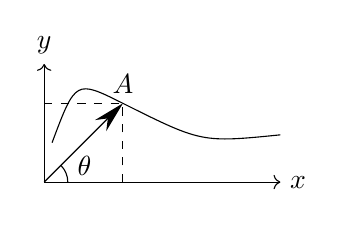
\begin{tikzpicture}
                \coordinate[label=right:$x$] (x) at (3,0);
                \coordinate[label=right:$\theta$] (theta) at (0.3,0.2);
                \coordinate[label=above:$y$] (y) at (0,1.5);
                \draw[->] (0,0) -- (x);
                \draw[->] (0,0) -- (y);
                \draw (0.1,0.5) .. controls (0.4,1.3) .. (1,1);
                \draw (1,1) .. controls (2,0.5) .. (3,0.6);
                \draw[\arrow] (0,0) -- (1,1);
                \coordinate[label=above:$A$] (A) at (1,1);
                \draw[dashed] (0,1) -- (A);
                \draw[dashed] (1,0) -- (A);
                \draw (0.3,0) arc (0:45:0.3);
            \end{tikzpicture}
        \]

        \[
            \left\{\begin{array}{l}x=r \cos \theta \\ y=r \sin \theta\end{array}\right.
        \]

        于是

        \[
            \overrightarrow{r} = x \overrightarrow{i} + y \overrightarrow{j} =
            r \cos \theta \overrightarrow{i}+ r \sin \theta \overrightarrow{j}
        \]
    \end{definition}

\subsubsection*{圆周运动的角量}

    \[
        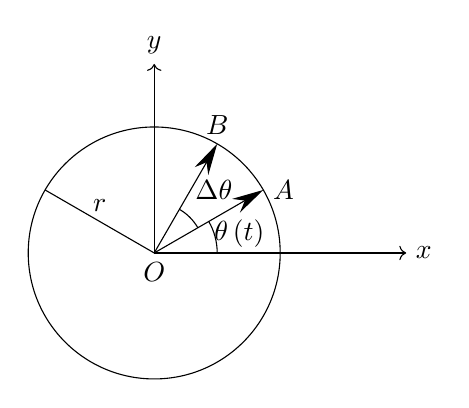
\begin{tikzpicture}[scale=0.8]
            \coordinate[label=right:$x$] (x) at (4,0);
            \coordinate[label=above:$y$] (y) at (0,3);
            \coordinate[label=below:$O$] (O) at (0,0);
            \coordinate[label=right:$A$] (A) at (1.732,1);
            \coordinate[label=above:$B$] (B) at (1,1.732);
            \coordinate[label=above:$r$] (r) at (-0.5*1.732,0.5);
            \coordinate[label={right:$\theta\left(t\right)$}] (theta) at (0.8,0.3);
            \coordinate[label=right:$\Delta \theta$] (Delta_theta) at (0.5,1);
            \draw[->] (O) -- (x);
            \draw[->] (O) -- (y);
            \draw (O) -- (-1.732,1);
            \draw[\arrow] (O) -- (A);
            \draw[\arrow] (O) -- (B);
            \draw (O) circle (2);
            \draw (1,0) arc (0:30:1);
            \draw (0.4*1.732,0.4) arc (30:60:0.8);
        \end{tikzpicture}
    \]

    角坐标\(\theta\left(t\right)\),角位移\(\Delta \theta = \theta\left(t\right) -
    \theta\left(t_0\right)\)。

    平均角速度
    
    \begin{align}
        \overline{\omega} = \frac{\Delta \theta}{\Delta t}
    \end{align}

    \vspace{1em}
    \begin{definition}[角速度]
    
        \begin{align}
            \omega = \lim_{\Delta t \rightarrow 0} \frac{\Delta \theta}{\Delta t}
            = \deriv{\theta}{t}
        \end{align}

        \(\omega\)是\textbf{赝矢量},方向与\(\rmd \theta\)一致,由右手螺旋定则确定,
        且总是垂直于圆平面,沿着圆周的轴线方向。
    \end{definition}

    平均角加速度
    
    \begin{align}
        \overline{\alpha} = \frac{\Delta \omega}{\Delta t}
    \end{align}
    
    \vspace{1em}
    \begin{definition}[角加速度]
    
        \begin{align}
            \alpha = \lim_{\Delta t \rightarrow 0} \frac{\Delta \omega}{\Delta t}
            = \deriv{\omega}{t} = \frac{\rmd^2 \theta}{\rmd t^2}
        \end{align}

    \end{definition}

\subsubsection*{角量与线量的关系}

    路程与角距离的关系

    \begin{align}
        \Delta s = r \Delta \theta
    \end{align}

    速率与角速度的关系

    \begin{align*}
        b = \lim_{\Delta t \rightarrow 0} \frac{\Delta s}{\Delta t}
        = r \lim_{\Delta t \rightarrow 0} \frac{\Delta \theta}{\Delta t}
    \end{align*}

    故

    \begin{align}
        v \left(t\right) = r \omega \left(t\right)
    \end{align}

    速度

    \begin{equation}
        \begin{aligned}
            \overrightarrow{v} &= \deriv{s}{t} \overrightarrow{e_t} \\
            &= v \overrightarrow{e_t} \\
            &= r \omega \overrightarrow{e_t}
        \end{aligned}
    \end{equation}

\subsubsection*{圆周运动的切向加速度和法向加速度}

    \[
        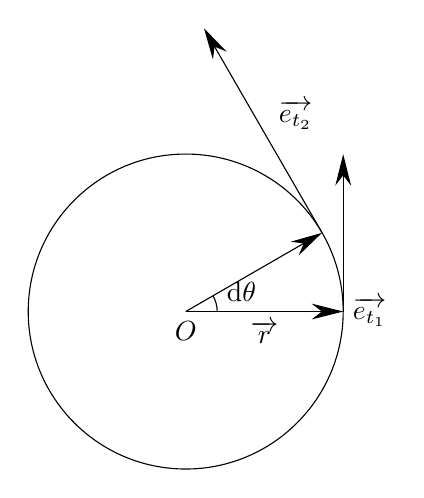
\begin{tikzpicture}
            \coordinate[label=below:$O$] (O) at (0,0);
            \coordinate[label=right:$\rmd \theta$] (dtheta) at (0.4,0.25);
            \coordinate[label=below:$\overrightarrow{r}$] (r) at (1,0);
            \coordinate[label=right:$\overrightarrow{e_{t_1}}$] (e_t_1) at (2,0);
            \coordinate[label=left:$\overrightarrow{e_{t_2}}$] (e_t_2) at (1.732,2.5);
            \draw (O) circle (2);
            \draw[\arrow] (O) -- (e_t_1);
            \draw[\arrow] (O) -- (1.732,1);
            \draw[\arrow] (e_t_1) -- (2,2);
            \draw[\arrow] (1.732,1) -- (1.732-1.5,1+1.5*1.732);
            \draw (0.4,0) arc (0:30:0.4);
        \end{tikzpicture}
    \]

    质点做变速圆周运动时

    \begin{equation}
        \overrightarrow{\alpha}=\deriv{\overrightarrow{v}}{t}=
        \frac{\rmd}{\rmd t}\left(v \overrightarrow{e}_t\right)=\deriv{\overrightarrow{v}}{t}
        \overrightarrow{e}_t+\overrightarrow{v} \deriv{\overrightarrow{e}_t}{t}
    \end{equation}

    \begin{equation}
        \alpha_{t} = \deriv{v}{t} = r \deriv{\omega}{t} = r \alpha
    \end{equation}

    因为\(\left|e_{t_1}\right| = \left|e_{t_2}\right| =1\),所以\(\left|\rmd \overrightarrow{e}\right|
    = \left|\overrightarrow{e_{t_1}}\right| \cdot \rmd \theta = \rmd \theta\)。

    当\(\rmd \theta \rightarrow 0\)时,\(\rmd \overrightarrow{e_{t}} \perp \overrightarrow{e_{t_1}}\),
    故\(\rmd \overrightarrow{e_{t}}\)的方向与\(\overrightarrow{e_{n}}\)方向相同,即

    \begin{align}
        \rmd \overrightarrow{e_{t}} = \rmd \theta \overrightarrow{e_n}
    \end{align}

    所以

    \[
        v \deriv{\overrightarrow{e_t}}{t} = v \deriv{\theta}{t} \overrightarrow{e_{n}} = v \omega
    \]

    于是

    \begin{align}
        \alpha_n &= \omega v \\
        &= \frac{v^2}{r}
    \end{align}

    综上所述,切向加速度\(\overrightarrow{\alpha_t} = \deriv{v}{t} \overrightarrow{e_t}, \;
    \alpha_t = \deriv{v}{t}\);法向加速度\(\overrightarrow{\alpha_t} = \frac{v^2}{r} \overrightarrow{e_n},
    \; \alpha_n = \frac{v^2}{r} = \omega^2r = \omega v\)。

\subsection{一般曲线运动}

    同圆周运动理知,

    \begin{align}
        \alpha_t = \deriv{v}{t}
    \end{align}

    \begin{align}
        \alpha_n = \frac{v^2}{\rho}\; \text{(\(\rho\)是曲率半径)}
    \end{align}

    而\(\overrightarrow{\alpha} = \overrightarrow{\alpha_t} + \overrightarrow{\alpha_n}\),所以

    \begin{align}
        \left|\overrightarrow{\alpha}\right| = \sqrt{\alpha_t^2 + \alpha_n^2}
    \end{align}

    自然坐标系下的加速度表达式:
    
    \begin{align}
        \overrightarrow{\alpha_t} = \deriv{v}{t} \overrightarrow{e_t} =
        \frac{\rmd^2 s}{\rmd t^2} \overrightarrow{e_t}
    \end{align}

    \begin{align}
        \overrightarrow{\alpha_n} = \frac{v^2}{\rho} \overrightarrow{e_n}
    \end{align}

\section{相对运动}

\subsection{时间与空间}

    在两个相对作直线运动的参考系中,时间的测量是绝对的,空间的测量也是绝对的,与参考系无关。

    时间和长度的的绝对性是经典力学或牛顿力学的基础。

    在两个相对作直线运动的参考系中, 时间的测量是绝对的,空间的测量也是绝对的, 与参考系无关, 时间和长度的的绝对性是经典力学或牛顿力学的基础。

\subsection{相对运动公式}

    \begin{wrapfigure}{r}{4cm}
        \centering
        \includegraphics[scale=0.3]{"Chapter 01 images/pic8.png"}
        % \caption{}
        \label{pic8}
    \end{wrapfigure}

    如右图,\(\overrightarrow{r_{OP}} = \overrightarrow{r_{OO^{'}}} + \overrightarrow{r_{O^{'}P}}\),

    对方程两边对时间求导数,得

    \begin{align*}
        \deriv{\overrightarrow{r_{OP}}}{t} = \deriv{\overrightarrow{r_{OO^{'}}}}{t} +
        \deriv{\overrightarrow{r_{O^{'}P}}}{t}
    \end{align*}

    即

    \begin{align}
        \overrightarrow{v_{P \rightarrow O}} = \overrightarrow{v_{P \rightarrow O^{'}}} +
        \overrightarrow{v_{O^{'} \rightarrow O}}
    \end{align}

    (绝对速度 = 相对速度 + 牵连速度)

    方程两边对时间求导数,得

    \begin{align}
        \overrightarrow{a_{P \rightarrow O}} = \overrightarrow{a_{P \rightarrow O^{'}}} +
        \overrightarrow{a_{O^{'} \rightarrow O}}
    \end{align}

    (绝对加速度 = 相对加速度 + 牵连加速度)

    如果\(\overrightarrow{u}\)是恒矢量,则\(\deriv{\overrightarrow{u}}{t} = 0\),
    \(\overrightarrow{a_{PO}} = \overrightarrow{a_{PO^{'}}}\),\(\overrightarrow{a_{O^{'}O}} = 0\)。

    注意:

    \begin{enumerate}
        \item 当\(\overrightarrow{u}\)接近光速时,速度变换、加速度变换不成立;
        \item 仅仅讨论\(\overrightarrow{u} = u_x \overrightarrow{i}\)的情况(\(u_x\)为常数),
        即水平方向有变换,其他方向上没有变换。
    \end{enumerate}

\subsection{伽利略速度变换}

    \vspace{1em}
    \begin{definition}[角加速度]

        \begin{align}
            \overrightarrow{v} = \overrightarrow{v}^{'} + \overrightarrow{u}
        \end{align}

        绝对速度\(\overrightarrow{v} = \deriv{\overrightarrow{r}}{t}\),相对速度\(\overrightarrow{v}^{'} =
        \deriv{\overrightarrow{r}^{'}}{t}\),牵连速度\(\overrightarrow{u}\)。

    \end{definition}

    \begin{figure}[!htbp]
        \centering
        \includegraphics[scale=0.4]{"Chapter 01 images/pic9.png"}
        % \caption{}
        \label{pic9}
    \end{figure}

    加速度关系:

    \begin{align}
        \deriv{\overrightarrow{v}}{t} = \deriv{\overrightarrow{v}^{'}}{t} + \deriv{\overrightarrow{u}}{t}
    \end{align}

    若\(\deriv{\overrightarrow{u}}{t} = 0\),则\(\overrightarrow{a} = \overrightarrow{a}^{'}\)

\section{例题}

    \begin{exercise}

        在离水面高为\(h\)的岸上,有人用绳拉船靠岸,如图所示。设人以匀速率\(v_{0}\)收绳,试求:
        当船距岸边\(x_{0}\)时,船的速度和加速度的大小各是多少?

        \[
            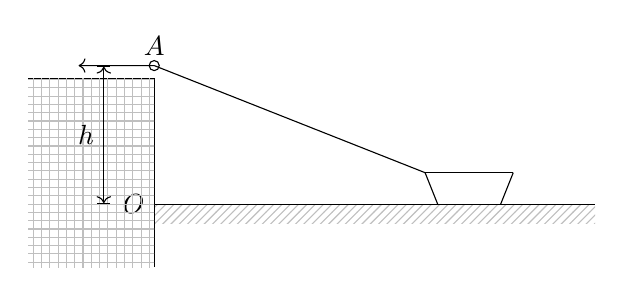
\begin{tikzpicture}[scale=0.8]
                \coordinate[label=left:$O$] (O) at (0,0);
                \coordinate[label=above:$A$] (A) at (0,2.2);
                \fill[pattern=north east lines, pattern color=gray!50] (0,0) rectangle (7,-0.3);
                \draw (0,-1) -- (0,2);
                \draw (O) -- (7,0);
                \draw (0,2) -- (-2,2);
                \fill[pattern=grid, pattern color=gray!50] (0,-1) rectangle (-2,2);
                \draw (A) circle (0.08);
                % 小船
                \draw (4.5,0) -- (5.5,0);
                \draw (4.5,0) -- (4.3,0.5);
                \draw (5.5,0) -- (5.7,0.5);
                \draw (4.3,0.5) -- (5.7,0.5);
                % 绳子
                \draw (A) -- (4.3,0.5);
                \draw[->] (A) -- (-1.2,2.2);
                % 尺寸标注
                \draw[|<->|] (-0.8,0) -- (-0.8,2.2) node[midway, left] {$h$};
            \end{tikzpicture}
        \]

    \end{exercise}
    \vspace{1em}

    \textbf{Solution}
    \vspace{1em}

    \textbf{Part One}

    建立如图所示的坐标系。

    \[
        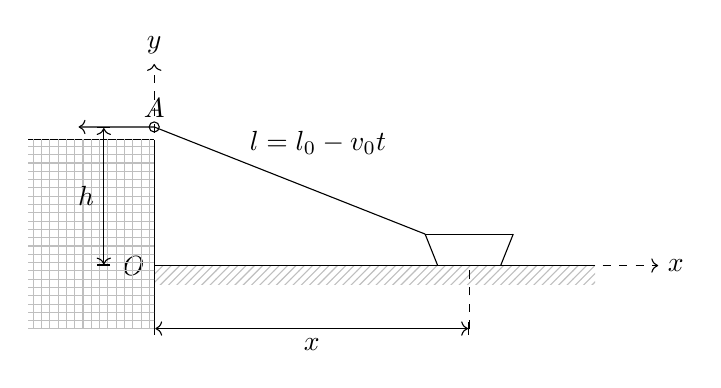
\begin{tikzpicture}[scale=0.8]
            \coordinate[label=left:$O$] (O) at (0,0);
            \coordinate[label=above:$A$] (A) at (0,2.2);
            \fill[pattern=north east lines, pattern color=gray!50] (0,0) rectangle (7,-0.3);
            \draw (0,-1) -- (0,2);
            \draw (O) -- (7,0);
            \draw (0,2) -- (-2,2);
            \fill[pattern=grid, pattern color=gray!50] (0,-1) rectangle (-2,2);
            \draw (A) circle (0.08);
            % 小船
            \draw (4.5,0) -- (5.5,0);
            \draw (4.5,0) -- (4.3,0.5);
            \draw (5.5,0) -- (5.7,0.5);
            \draw (4.3,0.5) -- (5.7,0.5);
            % 绳子
            \draw (A) -- (4.3,0.5);
            \draw[->] (A) -- (-1.2,2.2);
            \coordinate[label={above:$ l = l_{0} - v_{0}t $}] (rope) at (2.6,1.6);
            % 尺寸标注
            \draw[|<->|] (-0.8,0) -- (-0.8,2.2) node[midway, left] {$h$};
            \draw[|<->|] (0,-1) -- (5,-1) node[midway, below] {$x$};
            \draw[dashed] (5,-1) -- (5,0);
            % 坐标系
            \coordinate[label=right:$x$] (x) at (8,0);
            \coordinate[label=above:$y$] (y) at (0,3.2);
            \draw[->,dashed] (O) -- (x);
            \draw[->,dashed] (O) -- (y);
        \end{tikzpicture}
    \]

    设初始时刻,船与岸上\(A\)点之间的绳长为\(l_{0}\)。在任意时刻船离岸边的距离为\(x\),
    绳长为\(l_{0}\)。船在运动过程中,\(l\)和\(x\)均是时间\(t\)的函数。

    由题意,\(l = l_{0} - v_{0}t\),所以

    \[
        v_{0} = - \deriv{l}{t}
    \]

    又由几何关系

    \[
        l^{2} = x^{2} + h^{2}
    \]

    对上式两边同时对\(t\)求导,可得

    \[
        2 l \deriv{l}{t} = 2x \deriv{x}{t}
    \]

    则船的运动速度为

    \[
        v = \deriv{x}{t} = \frac{l}{x} \deriv{l}{t} = -\frac{l}{x} v_{0}
    \]
    \vspace{1em}

    \textbf{Part Two}

    再将速度对时间\(t\)求导,即可得到船的加速度为

    \[
        a = \deriv{v}{t} = - \frac{v_{0}}{x^{2}} \left(x \deriv{l}{t} - l \deriv{x}{t}\right)
        = -\frac{v_{0}^{2} h^{2}}{x^{3}}
    \]
    \vspace{1em}

    \textbf{Part Three}

    令\(x=x_{0}\),得船在离岸边为\(x_{0}\)时的速度和加速度分别为

    \[
        v = \frac{\sqrt{x_{0}^{2} + h^2}}{x_{0}} v_{0},\;
        a = -\frac{v_{0}^{2} h^{2}}{x_{0}^{3}}
    \]

\chapterimage{miku3.png} % Chapter heading image
\chapterspaceabove{6.25cm} % Whitespace from the top of the page to the chapter title on chapter pages
\chapterspacebelow{7.5cm} % Amount of vertical whitespace from the top margin to the start of the text on chapter pages

\chapter{牛顿运动定律}

\section{牛顿定律}

\subsection{牛顿第一定律}

    牛顿第一定律,又称惯性定律(law of inertia) 可表述如下:任何物体都将保持静止
    或匀速直线运动的状态,直至其他物体的作用强迫它改变这种状态时为止。

    即当\(\overrightarrow{F} = 0\)时,\(\overrightarrow{v}\)为恒矢量。

    牛顿第一定律指出了两个重要概念\textbf{惯性}和\textbf{力}。

\subsection{牛顿第二定律}

\subsubsection*{表述}

    动量为\(\overrightarrow{p}\)的物体, 在合外力\(\overrightarrow{F} \left(=\sum \overrightarrow{F_{i}}\right)\)
    的作用下,其动量随时间的变化率应当等于作用于物体的合外力,即

    \begin{align}
        \overrightarrow{F}\left(t\right) = \deriv{\overrightarrow{p}\left(t\right)}{t} =
        \deriv{\left(m\overrightarrow{v}\right)}{t}
    \end{align}

    (当\(v\ll c\)时,\(m\)为常量)

    于是有

    \begin{align}
        \overrightarrow{F} = m \deriv{\overrightarrow{v}}{t} = m \overrightarrow{a}
    \end{align}

    即可叙述如下:物体受到外力作用时,它所获得的加速度的大小与外力的大小成正比,
    与物体的质量成反比,加速度的方向与外力的方向相同。

\subsubsection*{牛顿运动定律的矢量性}

    由

    \begin{align*}
        \overrightarrow{F} = m \deriv{\overrightarrow{v}}{t} = m \overrightarrow{a}
    \end{align*}

    得

    \begin{equation}
        \overrightarrow{F}=m \frac{\mathrm{~d} v_x}{\mathrm{~d} t} \overrightarrow{i}+m \frac{\mathrm{~d} v_y}{\mathrm{~d} t} \overrightarrow{j}+m \frac{\mathrm{~d} v_z}{\mathrm{~d} t} \overrightarrow{k}
    \end{equation}

    即

    \begin{equation}
        \overrightarrow{F}=m a_x \overrightarrow{i}+m a_y \overrightarrow{j}+m a_z \overrightarrow{k}
    \end{equation}

    所以

    \begin{equation}
        \left\{\begin{array}{l}
        F_x=m a_x \\
        F_y=m a_y \\
        F_z=m a_z
        \end{array}\right.
    \end{equation}

\subsubsection*{自然坐标系中}

    \begin{equation}
        \overrightarrow{F}=m \overrightarrow{a}=
        m\left(\overrightarrow{a}_{\mathrm{t}}+\overrightarrow{a}_{\mathrm{n}}\right)=
        m \frac{\mathrm{~d} v}{\mathrm{~d} t} \overrightarrow{e}_{\mathrm{t}}+m \frac{v^2}{\rho} \overrightarrow{e}_{\mathrm{n}}
    \end{equation}

    也可写作

    \begin{equation}
        \left\{\begin{array}{l}
        F_{\mathrm{t}}=m \frac{\mathrm{~d} v}{\mathrm{~d} t}=m \frac{\mathrm{~d} s^2}{\mathrm{~d} t^2} \\
        F_{\mathrm{n}}=m \frac{v^2}{\rho}
        \end{array}\right.
    \end{equation}

    (\(\rho\)为\(A\)处曲线的曲率半径)

\subsubsection*{力的叠加原理}

    \begin{theorem}[力的叠加原理]

        当一个物体同时受到几个力的作用时,则这些力的合力产生的加逃度等于每个力单独作用时产生的矢
        量和,这一结论称为力的\textbf{独立性原理}或\textbf{力的叠加原理}。

        即

        \begin{equation}
            \begin{aligned}
            \overrightarrow{F} & =\overrightarrow{F}_1+\overrightarrow{F}_2+\cdots+\overrightarrow{F}_n=\sum \overrightarrow{F}_i \\
            & =m \overrightarrow{a}_1+m \overrightarrow{a}_2+\cdots+m \overrightarrow{a}_n=m \sum \overrightarrow{a}_i=m \overrightarrow{a}=m \frac{\mathrm{~d} v}{\mathrm{~d} t}
            \end{aligned}
        \end{equation}

\end{theorem}

\subsection{牛顿第三定律}

    两个物体之间作用力\(\overrightarrow{F}\)反和反作用力\(\overrightarrow{F}^{'}\), 
    沿同一直线,大小相等,方向相反,分别作用在两个物体上。

    作用力和反作用力的特点:

    \begin{enumerate}
        \item 作用力与反作用力总是同时存在、相互依存的。
        \item 作用力与反作用力分别作用在两个不同的物体上,虽然它们大小相等、方向相反,但不能互相抵消。
        \item 作用力与反作用力一定属于同一性质的力。
    \end{enumerate}

\subsection{总结}

    \begin{enumerate}
        \item 凡相对于惯性系作匀速直线运动的一切参考系都是惯性系;
        \item 对于不同惯性系,牛顿力学的规律都具有相同的形式,与惯性系的运动无关。
            (\textbf{伽利略相对性原理}或称\textbf{力学相对性原理})
    \end{enumerate}

\section{非惯性系、惯性力}

\subsection{惯性系、非惯性系}

    \vspace{1em}
    \begin{definition}[惯性系]

        牛顿运动定律在其中成立的参考系称为\textbf{惯性参考系},简称\textbf{惯性系}(inertial system)。

        “一个远离其他一切物体,而且没有自转的物体是惯性参照系,一切相对于该物体做匀速直线运动的参照系也是惯性参照系。
        牛顿定律就是在这样的参照系中成立。”——王燕生教授《大学物理问题讨论集》
        
    \end{definition}

    \textbf{举例}:

    \begin{enumerate}
        \item 地面参考系;
        \item 地心参考系;
        \item 日心参考系;
        \item FK4参考系:以选定的1535颗恒星的平均静止的位形作为基准的参考系,是比以上三个参考系都严格的惯性系。
    \end{enumerate}

    \vspace{1em}
    \begin{definition}[非惯性系]

        牛顿运动定律不成立的参考系称为\textbf{非惯性系}(non-inertial system)。
        
    \end{definition}

\subsection{惯性力}

\subsection{平动加速参考系、平动惯性力}

    假设非惯性系K'相对于惯性系K以加速度\(\overrightarrow{a}_{0}\)做平动,则由相对运动规律可知,质点相对于
    K'系和K系的加速度\(\overrightarrow{a}_{0}\)和\(\overrightarrow{a}\)满足:

    \begin{align}
        \overrightarrow{a} = \overrightarrow{a}_{0} + \overrightarrow{a}^{'}
    \end{align}

    惯性系中K,牛顿运动定律成立,即

    \begin{align}
        \overrightarrow{F} = m \overrightarrow{a} = m \left(\overrightarrow{a}_{0} + \overrightarrow{a}^{'}\right)
    \end{align}

    移项,得

    \begin{align}
        \overrightarrow{F} - m\overrightarrow{a}^{'} =  m \overrightarrow{a}_{0}
    \end{align}

    \vspace{1em}
    \begin{definition}[平动惯性力]

        \begin{align}
            \overrightarrow{F}_{0} = - m\overrightarrow{a}_{0}
        \end{align}
    \end{definition}

    将\(\overrightarrow{F}^{'} = \overrightarrow{F} + \overrightarrow{F}_{0} = \overrightarrow{F} -
    m \overrightarrow{a}_{0}\)看作非惯性参考系中受到的“合外力”,则在非惯性系K'中,牛顿第二定律在形式上成立:

    \begin{align}
        \overrightarrow{F}^{'} = \overrightarrow{F} + \overrightarrow{F}_{0} = m \overrightarrow{a}^{'}
    \end{align}

\subsubsection*{性质}

    不是真实的力,无施力物体,无反作用力是非惯性系加速度的反映。

\subsection{匀速转动参考系、惯性离心力}
    
    \begin{wrapfigure}{r}{4cm}
        \centering
        \includegraphics[scale=0.2]{"Chapter 02 images/pic1.jpg"}
        % \caption{}
        \label{pic1}
    \end{wrapfigure}

    匀速转动参考系也是一种常见的非惯性系。如右图所示,水平转盘以匀角速度\(\omega\)绕通过圆心的垂直轴转动,
    质量为\(m\)的小球用长度为\(R\)的绳子与转轴相连静止在圆盘上,并随圆盘一起转动。站在地面上的观察者看来,
    小球\(m\)以匀角速度\(\omega\)随圆盘一起转动,绳子施于小球的拉力\(\overrightarrow{F}_{r}\)
    提供了小球做匀速圆周运动时所需的向心力,即

    \begin{align}
        \overrightarrow{F}_{\mathrm{T}}=-m \frac{v^2}{R} \overrightarrow{e}_r=-m \omega^2 R \overrightarrow{e}_r
    \end{align}

    这表明在地面参考系中,小球的运动符合牛顿运动定律。

    但是,从圆盘这个转动参考系中来看,小球受到合外力\(\overrightarrow{F}_{T}\)的作用,但是静止不动。
    
    \vspace{1em}
    \begin{definition}[平动惯性力]
        
        为了在转动参考系中,仍然能够用牛顿运动定律解释该现象,需要引入一个虛拟的惯性力\(\overrightarrow{F}_{0}\),
        该力与绳子的拉力\(\overrightarrow{F}_{T}\)大小相等、方向相反,即

        \begin{equation}
            \overrightarrow{F}_0=-\overrightarrow{F}_{\mathrm{T}}=m \omega^2 R \overrightarrow{e}_r=-m \overrightarrow{a}_{\mathrm{n}}
        \end{equation}

        (\(\overrightarrow{e}_r\)表示径向单位矢量)

        称为惯性离心力(inertial centrifugal force)。

    \end{definition}

    于是引入惯性离心力后,在转动参考系中,牛顿运动定律在形式上成立。物体受到“合外力”为

    \begin{align*}
        \overrightarrow{F}_{T} + \overrightarrow{F}_{0} = \overrightarrow{0}
    \end{align*}

\section{例题}

\subsection*{解题思路}

    牛顿定律主要处理两类问题:

    \begin{enumerate}
        \item 质点;
        \item 质点系,尤其是连续分布的质点系。
    \end{enumerate}

    解题的基本思路:

    \begin{enumerate}
        \item 确定研究对象进行受力分析(隔离物体,画受力图);
        \item 取坐标系;
        \item 列方程(一般用分量式);
        \item 利用其它的约束条件列补充方程;
        \item 先用文字符号求解,后带入数据计算结果。
    \end{enumerate}

    \vspace{2em}
    \begin{exercise}

        一质量\(m\),半径\(r\)的球体在水中静止释放沉入水底。已知阻力\(F_{r} = - 6 \uppi r \eta v\),
        \(\eta\)为粘滞系数,求\(v\left(t\right)\)。

    \end{exercise}

        \textbf{Solution}
        \vspace{1em}


    \begin{wrapfigure}{r}{4cm}
        \centering
        \includegraphics[scale=0.3]{"Chapter 02 images/pic2.png"}
        % \caption{}
        \label{pic2}
    \end{wrapfigure}

    取坐标如图(\(\overrightarrow{F}_{B}\)为浮力),则

    $$
        m g-F_{\mathrm{B}}-6 \uppi \eta r v=m a
    $$

    令\(F_{0} = mg - F_{B}\),\(b = 6 \uppi \eta r\),于是

    $$
        F_0-b v=m \frac{\mathrm{~d} v}{\mathrm{~d} t}
    $$

    即

    $$
        \frac{\mathrm{d} v}{\mathrm{~d} t}=-\frac{b}{m}\left(v-\frac{F_0}{b}\right)
    $$

    两边同时积分:

    $$
        \int_0^v \frac{\rmd v}{v-\left(\frac{F_0}{b}\right)}=-\frac{b}{m} \int_0^t \rmd t
    $$

    得

    $$
        v=\frac{F_0}{b}\left[1-\mathrm{e}^{-\frac{b}{m} t}\right]
    $$

    则当\(t \rightarrow \infty\)时,\(v_{L} \rightarrow \frac{F_{0}}{b}\)(极限速度),
    当\(t = 3 \frac{b}{m}\)时,\(v = v_{L}\left(1-0.05\right) = 0.95 v_{L}\)。
    一般认为\(t \leq 3 \frac{b}{m}\)时,\(v = v_{L}\)

    \begin{figure}[!htbp]
        \centering
        \includegraphics[scale=0.3]{"Chapter 02 images/pic3.png"}
        % \caption{}
        \label{pic3}
    \end{figure}

    \begin{exercise}

        质量为\(m\)的物体,由地面以初速度\(v_{0}\)竖直向上发射,物体受到空气阻力大小\(F_{r} = kv\)。
        试求:

        \begin{enumerate}
            \item 物体发射到最大高度所需要的时间;
            \item 物体能到达的最大高度。
        \end{enumerate}

    \end{exercise}

    \textbf{Solution}
    \vspace{1em}

    \textbf{Part One}
    \vspace{1em}

    \begin{wrapfigure}{r}{4cm}
        \centering
        \includegraphics[scale=0.3]{"Chapter 02 images/pic4.png"}
        % \caption{}
        \label{pic4}
    \end{wrapfigure}

    物体在向上发射的过程中,受到重力和阻力作用,方向均与速度方向相反。以竖直向上作为正方向,
    由牛顿运动定律可得

    \begin{equation}
        -m g-k v=m \frac{\mathrm{~d} v}{\mathrm{~d} t}
        \label{Problem-2-1}
    \end{equation}

    对上式分离变量并取定积分,同时注意到物体到达最大高度时\(v=0\),即

    $$
        \int_0^t \mathrm{~d} t=\int_{v_0}^0-\frac{m}{m g+k v} \mathrm{~d} v
    $$

    积分得物体达到最大高度所需的时间为

    $$
        t=\frac{m}{k} \ln \frac{m g+k v_0}{m g}
    $$

    \textbf{Part Two}
    \vspace{1em}

    利用$\dfrac{\mathrm{d} v}{\mathrm{~d} t}=v \dfrac{\mathrm{~d} v}{\mathrm{~d} y}$代入\ref{Problem-2-1}式,可得

    $$
        -m g-k v=m \frac{\mathrm{~d} v}{\mathrm{~d} t}
    $$

    分离变量并取定积分,即

    $$
        \int_0^y \mathrm{~d} y=\int_{v_0}^0-\frac{m v}{m g+k v} \mathrm{~d} v
    $$

    所以物体可达到的最大高度为

    $$
        y=\frac{m}{k}\left(v_0-\frac{m g}{k} \ln \frac{m g+k v_0}{m g}\right)
    $$

\subsection{Problem 3}

    \begin{exercise}

        一条质量均匀分布的绳子,总质量为\(M\)、长度为\(L\),一端拴在竖直转轴\(OO^{'}\)\\上,
        并以恒定的角速度\(\omega\)在水平面上旋转。设转动过程中绳子始终伸直不打弯,
        且忽略重力的影响,求距离转轴为\(r\)处绳中的张力\(T\left(r\right)\)。

        \[
            \includegraphics[scale=0.18]{"Chapter 02 images/pic5.png"}
            % \caption{}
            \label{pic5}
        \]

    \end{exercise}

    \textbf{Solution}
    \vspace{1em}

    在距离转轴为\(r\)处,取一个长为\(\rmd r\)的一小段绳子,其质量为\(\frac{M}{L} \rmd r\),
    其两端受力如图所示,由于该段绳子作圆周运动,所以由牛顿第二定律得

    \begin{wrapfigure}{r}{4cm}
        \centering
        \includegraphics[scale=0.18]{"Chapter 02 images/pic6.png"}
        % \caption{}
        \label{pic6}
    \end{wrapfigure}

    $$
        T(r)-T(r+\rmd r)=\rmd m \cdot a_n=\frac{M}{L} \rmd r
    $$

    令

    $$
        T(r)-T(r+\rmd r)=\rmd m \cdot a_n=\frac{M}{L} \rmd r
    $$

    得

    $$
        \rmd T=-\frac{M \omega^2}{L} r \rmd r
    $$

    式中\(\rmd T\)就是该小段绳子所受的合外力,“\(-\)”号表示该段绳子受到的合外力的方向与矢径
    \(r\)相反,指向圆心。根据力的叠加原理,离轴\(r\)处绳中的张力就是\(r\)以外所有小段绳子所受的
    合力的绝对值之和,即

    $$
        T(r)=\int|\mathrm{d} T|=\int_r^L \frac{M \omega^2}{L} r \mathrm{~d} r=\frac{M \omega^2}{2 L}\left(L^2-r^2\right)
    $$

\chapterimage{miku1.jpg} % Chapter heading image
\chapterspaceabove{6.25cm} % Whitespace from the top of the page to the chapter title on chapter pages
\chapterspacebelow{7.5cm} % Amount of vertical whitespace from the top margin to the start of the text on chapter pages

\chapter{运动的守恒定律}

    \textbf{守恒量}:对于物体系统内发生的各种过程,如果某物理量始终保持不变,
    该物理量就叫做守恒量。

    \textbf{守恒定律}:由宏观现象总结出来的最深刻、最简洁的自然规律。
    (动量守恒定律、机械能守恒定律、能量守恒定律和角动量守恒定律等)

\section{质点和质点系的动量定理}

    力的\textbf{累积}效应:

    \begin{enumerate}
        \item \(\overrightarrow{F}\left(t\right)\)对\(t\)累计\(\rightarrow \overrightarrow{I},\; \Delta \overrightarrow{p}\)
        \item \(\overrightarrow{F}\)对\(\overrightarrow{t}\)累计\(\rightarrow W,\; \Delta E\)
    \end{enumerate}

    \subsection{冲量、质点的动量定理}

    \subsubsection*{动量}

    \vspace{1em}
    \begin{definition}[动量]

        \begin{equation}
            \overrightarrow{p} = m\overrightarrow{v}
        \end{equation}

    \end{definition}

    故

    \begin{equation}
        \overrightarrow{F} = \deriv{\overrightarrow{p}}{t} = \deriv{\left(m\overrightarrow{v}\right)}{t}
    \end{equation}

    即

    $$
        \overrightarrow{F} \mathrm{~d} t=\mathrm{d} \overrightarrow{p}=\mathrm{d}(m \overrightarrow{v})
    $$

    两边同时积分:

    $$
        \int_{t_1}^{t_2} \overrightarrow{F} \mathrm{~d} t=\overrightarrow{p}_2-\overrightarrow{p}_1=
        m \overrightarrow{v}_2-m \overrightarrow{v}_1
    $$

    \subsubsection*{冲量}

    \vspace{1em}
    \begin{definition}[冲量]

        \begin{equation}
            \overrightarrow{I} = \int_{t_1}^{t_2} \overrightarrow{F} \rmd t
        \end{equation}

    \end{definition}

    \vspace{1em}
    \begin{theorem}[动量定理]

        在给定的时间间隔内,外力作用在质点上的冲量等于质点在此时间内动量的增量

        微分形式:

        \begin{equation}
            \overrightarrow{F} \mathrm{~d} t=\mathrm{d} \overrightarrow{p}=\mathrm{d}(m \overrightarrow{v})
        \end{equation}

        积分形式:

        \begin{equation}
            \int_{t_1}^{t_2} \overrightarrow{F} \mathrm{~d} t = m \overrightarrow{v}_2-m \overrightarrow{v}_1
        \end{equation}

        分量形式:

        \begin{equation}
            \left\{\begin{array}{l}
            I_x=\int_{t_1}^{t_2} F_x \mathrm{~d} t=m v_{2 x}-m v_{1 x} \\
            I_y=\int_{t_1}^{t_2} F_y \mathrm{~d} t=m v_{2 y}-m v_{1 y} \\
            I_z=\int_{t_1}^{t_2} F_z \mathrm{~d} t=m v_{2 z}-m v_{1 z}
            \end{array}\right.
        \end{equation}

        可知,某方向受到冲量,该方向上的动量就增加。

    \end{theorem}

    \subsection{质点系的动量定理}

    \vspace{1em}
    \begin{theorem}[质点系的动量定理]

        作用于系统的合外力的冲量等于系统动量的增量。

        \begin{equation}
            \int_{t_1}^{t_2} \overrightarrow{F}^{\mathrm{ex}} \mathrm{~d} t=
            \sum_{i=1}^n m_i \overrightarrow{v}_i-\sum_{i=1}^n m_i \overrightarrow{v}_{i 0}
            =\overrightarrow{p}-\overrightarrow{p}_0
        \end{equation}

        或

        \[
            \overrightarrow{I} = \overrightarrow{p} - \overrightarrow{p_{0}}
        \]

    \end{theorem}

    \begin{enumerate}
        \item 若\(\overrightarrow{F}\)为恒力,则\(\overrightarrow{I} = \overrightarrow{F} \Delta t\)
        \item 若\(\overrightarrow{F}\)为变力,则\(\overrightarrow{I} =
            \int_{t_1}^{t_2} \overrightarrow{F} \rmd t = \overline{\overrightarrow{F}}\left(t_2-t_1\right)\)
    \end{enumerate}

    \textbf{动量定理常应用于碰撞问题}。

    $$
    \overline{\overrightarrow{F}}=\frac{\int_{t_1}^{t_2} \overrightarrow{F} \mathrm{~d} t}{t_2-t_1}
    =\frac{m \overrightarrow{v}_2-m \overrightarrow{v}_1}{t_2-t_1}
    $$

    \section{动量守恒定律、动能定理}

    \subsection{动量守恒定律}

    由质点系动量定理:

    $$
        \overrightarrow{I}=\int_{t_0}^t \sum_i \overrightarrow{F}_i^{\mathrm{ex}} \mathrm{~d} t=
        \sum_i \overrightarrow{p}_i-\sum_i \overrightarrow{p}_{i 0}
    $$

    若质点系所受的合外力\(\overrightarrow{F}^{\mathrm{ex}} = \overrightarrow{F}_i^{\mathrm{ex}}= 0\)

    则系统的总动量不变。——动量守恒定律

    \begin{enumerate}
        \item 系统的总动量不变,但系统内任意物体的动量是可以变的;
        \item 守恒条件:合外力为零。\\
            \(\overrightarrow{F}^{\mathrm{ex}} = \sum_i \overrightarrow{F}_i^{\mathrm{ex}}= 0\)\\
            当\(\overrightarrow{F}^{\mathrm{ex}} \ll \overrightarrow{F}^{\mathrm{in}}\),
            可近似地认为系统总动量守恒。
        \item 若\(\overrightarrow{F}^{\mathrm{ex}} = \sum_i \overrightarrow{F}_i^{\mathrm{ex}}\neq 0\),
            但满足\(F_{x}^{\mathrm{ex}} = 0\),则有$p_x=\sum_i m_i v_{i x}=C_x$
            即

            \begin{equation}
                \begin{cases}F_x^{\mathrm{ex}}=0, & p_x=\sum_i m_i v_{i x}=C_x \\
                F_y^{\mathrm{ex}}=0, & p_y=\sum_i^i m_i v_{i y}=C_y \\
                F_z^{\mathrm{ex}}=0, & p_z=\sum_i m_i v_{i z}=C_z\end{cases}
            \end{equation}
        \item 动量守恒定律是物理学最普遍、最基本的定律之一。
    \end{enumerate}

    \subsection{功}

    物体在力\(\overrightarrow{F}\)的作用下移动\(\Delta \overrightarrow{r} \rightarrow\)做功\(W\)

    \subsubsection*{恒力作用下的功}

    \begin{equation}
        \begin{aligned}
        W & =F \cos \alpha \cdot|\Delta \overrightarrow{r}| \\
        & =\overrightarrow{F} \cdot \Delta \overrightarrow{r}
        \end{aligned}
    \end{equation}

    \subsubsection*{变力作用下的功}

    \begin{wrapfigure}{r}{4cm}
        \centering
        \includegraphics[scale=0.2]{"Chapter 03 images/pic1.png"}
        % \caption{}
        \label{pic1}
    \end{wrapfigure}

    元位移\(\rmd \overrightarrow{r}\)、元路程\(\rmd s\)

    则元功\(\rmd W = \overrightarrow{F} \cdot \rmd \overrightarrow{r} =
    F \cos \alpha \rmd s\)

    积分:

    \begin{align}
        W=\int_A^B \overrightarrow{F} \cdot \rmd \overrightarrow{r}=\int_A^B F \cos \alpha \mathrm{~d} s
    \end{align}

    \begin{enumerate}
        \item 功的正负
            $$
                \begin{cases}0^{\circ}<\alpha<90^{\circ}, & \mathrm{d} W>0 \\
                90^{\circ}<\alpha<180^{\circ}, & \mathrm{d} W<0 \\
                \alpha=90^{\circ}, \text{即} \overrightarrow{F} \perp \rmd \overrightarrow{r}, & \rmd W=0\end{cases}
            $$
        \item 做功的图示
            \[
                \includegraphics[scale=0.2]{"Chapter 03 images/pic2.png"}
            \]
        \item 功是一个过程量,与路径有关。
        \item 合力的功,等于各分力的功的\textbf{代数和}
            \begin{align*}
                \overrightarrow{F}=F_x \overrightarrow{i}+F_y \overrightarrow{j}+F_z \overrightarrow{k} \\
                \mathrm{~d} \overrightarrow{r}=\mathrm{d} x \overrightarrow{i}+\mathrm{d} y \overrightarrow{j}+\mathrm{d} z \overrightarrow{k}
            \end{align*}
            则
            \begin{align*}
                W=\int_A^B \overrightarrow{F} \cdot \mathrm{~d} \overrightarrow{r}=
                \int_A^B\left(F_x \mathrm{~d} x+F_y \mathrm{~d} y+F_z \mathrm{~d} z\right)
            \end{align*}
            又有$W_x=\int_{x_1}^{x_B} F_x \mathrm{~d} x$、$W_y=\int_{y_1}^{y_B} F_y \mathrm{~d} y$、
            $W_z=\int_{z_1}^{z_B} F_z\mathrm{~d} z$。\\
            于是
            \[
                W = W_x + W_y + W_z
            \]

    \end{enumerate}

    \subsection{功率}

    \textbf{平均功率}$\overline{P}=\frac{\Delta W}{\Delta t}$

    \vspace{1em}
    \begin{definition}[瞬时功率]

        \begin{align}
            P=\lim _{\Delta t \rightarrow 0} \frac{\Delta W}{\Delta t}=\frac{\mathrm{d} W}{\mathrm{~d} t}=\overrightarrow{F} \cdot \overrightarrow{v}
        \end{align}

        即

        \begin{align}
            P = Fv\cos\alpha
        \end{align}

    \end{definition}

    \subsection{动能定理}

    \vspace{1em}
    \begin{theorem}[质点的动能定理]

        $$
        \begin{aligned}
            W & =\int \overrightarrow{F} \cdot \mathrm{~d} \overrightarrow{r} \\
            & =\int F_{\mathrm{t}}|\mathrm{~d} \overrightarrow{r}|=\int F_{\mathrm{t}} \mathrm{~d} s
        \end{aligned}
        $$

        而

        $$
            F_{\mathrm{t}}=m \frac{\mathrm{~d} v}{\mathrm{~d} t}
        $$

        于是

        $$
            \begin{aligned}
            W & =\int_{v_1}^{v_2} m v \mathrm{~d} v \\
            & =\frac{1}{2} m v_2^2-\frac{1}{2} m v_1^2
            \end{aligned}
        $$

        即

        \begin{equation}
            W=\frac{1}{2} m v_2^2-\frac{1}{2} m v_1^2=E_{\mathrm{k} 2}-E_{\mathrm{k} 1}
        \end{equation}

        \[
            \includegraphics[scale=0.2]{"Chapter 03 images/pic3.png"}
            % \caption{}
            \label{pic3}
        \]

        合外力对质点所作的功,等于质点动能的增量。——质点的动能定理

    \end{theorem}

    \begin{enumerate}
        \item 功是\textbf{过程量},动能是\textbf{状态量};
        \item 功和动能依赖于惯性系的选取,但对不同惯性系动能定理形式相同。
    \end{enumerate}

    \subsubsection*{质点系的动能定理}

    \textbf{质点系}:由有限个或无限个质点组成的系统。(可以是固体也可以是液体,它概括了力学中最普遍的研究对象)

    \textbf{内力和外力}:质点系以外的物体作用于质点系内各质点的力称为外力,
    质点系内各质点之问的相互作用力称为内力,外力和内力的区分完全洪定于质点系(研究对象)的选取。

    \textbf{质点系内力的功}:一切内力矢量和恒等于零。但一般情烷下,所有内力作功的总和并不为零。
    例如,两个彼此相互吸引的物体,移动一段位移,都作正功。

    \textbf{质点系的动能定理}

    由质点动能定理$W=E_{k 2}-E_{k 1}=\Delta E_k$

    得

    \begin{equation}
        W_e+W_i=\sum_i\left(\frac{1}{2} m_i v_{i 2}^2-\frac{1}{2} m_i v_{i 1}^2\right)=E_{k 2}-E_{k 1}=\Delta E_k
    \end{equation}

    意义:合外力所做的功等于系统动能的增量。

    \section{保守力、势能、成对力的功}

    \subsection{保守力}

    \subsubsection*{万有引力}

    \begin{wrapfigure}{r}{4cm}
        \centering
        \includegraphics[scale=0.2]{"Chapter 03 images/pic4.png"}
        % \caption{}
        \label{pic4}
    \end{wrapfigure}

    \(m_{E}\)对\(m\)的万有引力为

    $$
        \overrightarrow{F}=-G \frac{m_{E} m}{r^2} \overrightarrow{e}_r
    $$

    \(m\)移动\(\rmd \overrightarrow{r}\)时,\(\overrightarrow{F}\)做元功为

    $$
        \rmd W = \overrightarrow{F} \cdot \rmd \overrightarrow{r}
        =-G \frac{m_{E} m}{r^2} \overrightarrow{e}_r \cdot \rmd \overrightarrow{r}
    $$

    \(m\)从\(A\)到\(B\)时,\(\overrightarrow{F}\)做功为

    $$
    W=\int \overrightarrow{F} \cdot \rmd \overrightarrow{r}
    =\int_A^B-G \frac{m_{E} m}{r^2} \overrightarrow{e}_r \cdot \rmd \overrightarrow{r}
    $$

    \begin{wrapfigure}{r}{4cm}
        \centering
        \includegraphics[scale=0.15]{"Chapter 03 images/pic6.png"}
        % \caption{}
        \label{pic6}
    \end{wrapfigure}

    其中,$\overrightarrow{e}_r \cdot \mathrm{~d} \overrightarrow{r}=
    \left|\overrightarrow{e}_r\right| \cdot|\mathrm{d} \overrightarrow{r}| \cos \alpha=\mathrm{d} r$

    即

    $$
        W=\int_{r_A}^{r_B} \left(-G \frac{m_E m}{r^2}\right) \rmd r
    $$

    于是

    \begin{equation}
        W=G m_{E} m\left(\frac{1}{r_B}-\frac{1}{r_A}\right)
    \end{equation}

    \textbf{做功特点}:做功大小只与物体的始末位置有关,与路径无关。

    \subsubsection*{弹性力做功}

    \begin{wrapfigure}{r}{4cm}
        \centering
        \includegraphics[scale=0.12]{"Chapter 03 images/pic5.png"}
        % \caption{}
        \label{pic5}
    \end{wrapfigure}

    弹性力\(\overrightarrow{F} = -kx\overrightarrow{i}\),则元功

    \[
        \rmd W = -kx \rmd x
    \]

    于是

    \begin{equation}
        W=\int_{x_a}^{x_b} F \mathrm{~d} x=\int_{x_a}^{x_b}-k x \mathrm{~d} x=-\left(\frac{1}{2} k x_b^2-\frac{1}{2} k x_a^2\right)
    \end{equation}

    \textbf{做功特点}:做功大小只与物体的始末位置有关,与路径无关。

    \subsubsection*{保守力与非保守力的定义}

    \textbf{保守力}:作功与路径无关,仅决定于始、末位置的力。

    质点沿任意闭合路径运动一周时,保守力对它作功为零。

    \textbf{非保守力}:所作的功与路径有关的力。(如摩擦力)

    \vspace{1em}
    \begin{definition}[势能]

        因相对位置而具有的作功本领称为势能或位能(因有速度而具有的作功本领称为动能)。
        势能与质点的位置有关。

    \end{definition}

    如引力势能

    \[
        E_{\mathrm{p}} = -G \frac{m_{E}m}{r}
    \]

    如弹性势能

    \[
        E_{\mathrm{p}} = \frac{1}{2}kx^2
    \]

    \subsubsection*{保守力做功}

    \textbf{保守力做的功等于势能的减少},即

    \begin{equation}
        W =-\left(E_{\mathrm{p} 2}-E_{\mathrm{p} 1}\right)=-\Delta E_{\mathrm{p}}
    \end{equation}

    \subsubsection*{保守力做功势能的计算}

    令\(E_{\mathrm{p0}} = 0\),则

    \begin{equation}
        E_{\mathrm{p}}(x, y, z)=\int_{(x, y, z)}^{E_{\mathrm{p} 0}=0} \overrightarrow{F} \cdot \mathrm{~d} \overrightarrow{r}
    \end{equation}

    \begin{enumerate}
        \item 势能是\textbf{状态的函数},$E_{\mathrm{p}}=E_{\mathrm{p}}(x, y, z)$;
        \item 势能具有\textbf{相对性},势能大小与势能零点的选取有关;
        \item 势能是\textbf{属于系统}的;
        \item \textbf{势能差}与势能零点的选取无关。
    \end{enumerate}

    \subsubsection*{势能曲线}

    \begin{figure}[htbp]
        \centering
        \subfigure
        {
            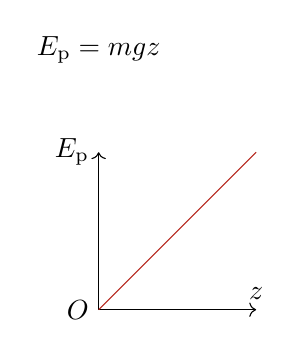
\begin{tikzpicture}
                \coordinate[label=left:$E_{\mathrm{p}}$] (E_p) at (0,2);
                \coordinate[label=above:$z$] (z) at (2,0);
                \coordinate[label=left:$O$] (O) at (0,0);
                \coordinate[label={above:$E_{\mathrm{p}} = mg z$}] (formula) at (0,3);
                \draw[->] (O) -- (z);
                \draw[->] (O) -- (E_p);
                \draw[domain=0:2,BrickRed] plot(\x,{\x});
            \end{tikzpicture}
        }
        \subfigure
        {
            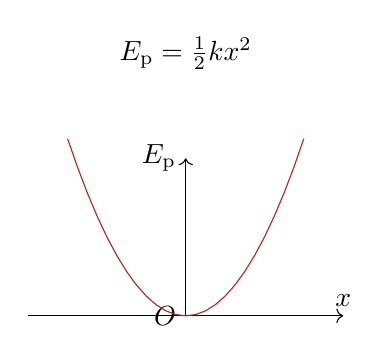
\begin{tikzpicture}
                \coordinate[label=left:$E_{\mathrm{p}}$] (E_p) at (0,2);
                \coordinate[label=above:$x$] (x) at (2,0);
                \coordinate[label=left:$O$] (O) at (0,0);
                \coordinate[label={above:$E_{\mathrm{p}} = \frac{1}{2}kx^2$}] (formula) at (0,3);
                \draw[->] (-2,0) -- (x);
                \draw[->] (O) -- (E_p);
                \draw[domain=-1.5:1.5,BrickRed] plot(\x,{\x*\x});
            \end{tikzpicture}
        }
        \subfigure
        {
            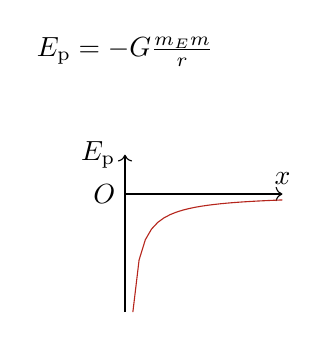
\begin{tikzpicture}
                \coordinate[label=left:$E_{\mathrm{p}}$] (E_p) at (0,0.5);
                \coordinate[label=above:$x$] (x) at (2,0);
                \coordinate[label=left:$O$] (O) at (0,0);
                \coordinate[label={above:$E_{\mathrm{p}} = -G \frac{m_{E}m}{r}$}] (formula) at (0,1.5);
                \draw[->] (O) -- (x);
                \draw[->] (0,-1.5) -- (E_p);
                \draw[domain=0.1:2,BrickRed] plot(\x,{-0.15/\x});
            \end{tikzpicture}
        }
        % \caption{}
    \end{figure}

    把势能和相对位置的关系绘成曲线,便得到势能曲线。
            
    通过势能曲线,可以显示出系统总机械能,动能和势能间的关系
    $E=E_k+E_p$,由 $E_{\mathrm{k}} \geq 0$ ,可以根据曲线的形状讨论物体的运动。

    \subsubsection*{由势能求表达式}

    可以根据势能\(E_{\mathrm{p}}\left(x,y,z\right)\)的情况,判断物体在各个位置所受保守力的大小和方向:

    $$
        \rmd W=F_x \rmd x=-\rmd E_p
    $$

    则

    \begin{equation}
        F_x=-\frac{\rmd E_p}{\rmd x}
    \end{equation}

    如果势能是位置\(\left(x,y,z\right)\)的多元函数,则

    \begin{equation}
        \overrightarrow{F}=F_x \overrightarrow{i}+F_y \overrightarrow{j}+F_z \overrightarrow{k}=
        -\left(\frac{\partial E_p}{\partial x} \overrightarrow{i}+\frac{\partial E_p}{\partial y} \overrightarrow{j}+\frac{\partial E_p}{\partial z} \overrightarrow{k}\right)
    \end{equation}

    \subsection{成对的力的功}

    力总是成对的,无论是保守力还是非保守力。

    设质量为$m_1$和$m_2$的两个物体分别受到 $F_1$ 和 $F_2$ 的力,
    且 $\overrightarrow{F}_1=-\overrightarrow{F}_2$在$\rmd t$时间内位移为 $\rmd r_1$
    和 $\rmd r_2$ ,质点 2 相对于质点 1 的相对位移 $\rmd \overrightarrow{r}^{\prime}$有
    $\rmd \overrightarrow{r}_2=d \overrightarrow{r}_1+\rmd r^{\prime}$ 则元功为:

    $$
        \begin{aligned}
        & \rmd W_1=\overrightarrow{F}_1 \cdot \rmd \overrightarrow{r}_1 \\
        & \rmd W_2=\overrightarrow{F}_2 \cdot \rmd \overrightarrow{r}_2
        \end{aligned}
    $$

    这一对力所作元功之和为:

    $$
    \begin{aligned}
        & \rmd W=\overrightarrow{F}_1 \cdot \rmd \overrightarrow{r}_1+\overrightarrow{F}_2 \cdot \rmd \overrightarrow{r}_2=\overrightarrow{F}_1 \cdot\rmd\overrightarrow{r}_1+\overrightarrow{F}_2 \cdot\left(d \overrightarrow{r}_1+d \overrightarrow{r}^{\prime}\right) \\
        & =\left(-\overrightarrow{F}_2+\overrightarrow{F}_2\right) \cdot\rmd\overrightarrow{r}_1+\overrightarrow{F}_2 \cdot\rmd\overrightarrow{r}^{\prime} \quad \\
        & =\overrightarrow{F}_2 \cdot\rmd\overrightarrow{r}^{\prime}
    \end{aligned}
    $$

    \begin{enumerate}
        \item 成对力的功只与作用力和相对位移有关;
        \item 成对力的总功具有与参考系选择无关的不变性质。\\
            为方便起见,计算时常认为其中一个质点静止,并以该质点所在位置为原点,
            再计算另一质点受力所做的功,这就是一对力的功。
        \item 在无相对位移或相对位移与一对力垂直的情况下,一对力的功必为零。
    \end{enumerate}

    \section{功能原理、机械能守恒定律}

    \subsection{质点系功能原理}

    \textbf{系统的机械能}:动能与势能的综合称为机械能,即

    \[
        E = E_{\mathrm{k}} + E_{\mathrm{p}}
    \]

    \textbf{内力的功可分为}:保守内力的功和非保守内力功

    \[
        W^{\mathrm{in}} = \sum_{i} W_{i}^{\mathrm{in}} =
        W_{\mathrm{c}}^{\mathrm{in}} + W_{\mathrm{nc}}^{\mathrm{in}}
    \]

    由势能的定义,保守内力的功总等于系统势能的减少:

    \[
        W_{\mathrm{c}}^{\mathrm{in}} = - \Delta E_{\mathrm{p}}
    \]

    \begin{theorem}[系统的功能原理]

        由质点系的动能定理:

        \[
            W^{\mathrm{ex}} + W^{\mathrm{in}} = W^{\mathrm{ex}} + W_{\mathrm{c}}^{\mathrm{in}}
            + W_{\mathrm{nc}}^{\mathrm{in}} = W^{\mathrm{ex}} - \Delta E_{\mathrm{p}} +
            W_{\mathrm{nc}}^{\mathrm{in}} = \Delta E_{\mathrm{k}}
        \]

        于是,

        \begin{align}
            \Delta E = \Delta E_{\mathrm{k}} + \Delta E_{\mathrm{p}} =
            W^{\mathrm{ex}} + W_{\mathrm{nc}}^{\mathrm{in}}
        \end{align}

        在选定的质点系内,在任一过程中,质点系总机械能的增量等于\textbf{所有外力}的功与\textbf{非保守内力}的功的代数和。

        非保守内力的功将导致机械能与其他形式的能量转换。

    \end{theorem}

    \subsection{机械能守恒定律}

    \begin{theorem}[机械能守恒定律]

        由功能原理:$\Delta E = \Delta E_{\mathrm{k}} + \Delta E_{\mathrm{p}} =
        W^{\mathrm{ex}} + W_{\mathrm{nc}}^{\mathrm{in}}$。

        如果$W^{\mathrm{ex}} + W_{\mathrm{nc}}^{\mathrm{in}} = 0$,则

        \[
            \Delta E = \Delta E_{\mathrm{k}} + \Delta E_{\mathrm{p}} = 0
        \]

        即,如是系统内只有保守内力做功,其他内力和一切外力都不做功,或元功之和为零,
        则系统内各物体的动能和势能可以相互转换,但总机械能保持不变。

    \end{theorem}

    \begin{enumerate}
        \item 质点系的机械能守恒的条件是:在一个过程中,既没有外力做功,也没有非保守内力(如摩擦力、爆炸力、流体的黏性阻力等耗散力)做功,或者外力和非保守内力做的总功为零。
        \item 在满足守恒条件时,质点系的总机械能可以在动能和系统势能之间转化,也可以在系统内各物体之问转移,但在转化和转移过程中保特总机械能不变。
    \end{enumerate}

    \subsection{能量守恒定律}

    \begin{theorem}[能量守恒定律]

        对于一个不受外界影响的封闭系统(有时也称为狐立系统),系统内各种不同形式的能量可以互相转化,也可以从系统的一部分转移到另一部分,
        但不论系统内发生什么过程,能量既不会消失也不会产生,系统的总能量恒定不变。这就是能量守恒定律 (law of conservation of energy)。

    \end{theorem}

    \subsection{动量与能量的比较}

    \begin{table}[htbp]
        \centering
        \begin{tabular}{|l|ll|}
            \hline
            \textbf{物理量} & \multicolumn{1}{l|}{\textbf{动量(momentum)}}                    & \textbf{能量(kinetic energy)}      \\ \hline
            表达式          & \multicolumn{1}{l|}{\(\overrightarrow{p} = m\overrightarrow{v}\)} & \(E_{\mathrm{k}} = \frac{1}{2}mv^2\) \\ \hline
            单位  & \multicolumn{1}{l|}{\(\mathrm{kg \cdot m / s}\)} & \(\mathrm{J}\)                  \\ \hline
            性质  & \multicolumn{1}{l|}{矢量}                      & 标量                          \\ \hline
            关系  & \multicolumn{2}{c|}{\(\dfrac{p^2}{2m} = E_{\mathrm{k}}\)}                       \\ \hline
            变化量 & \multicolumn{1}{l|}{\(\Delta p\)由力的冲量决定}         & \(\Delta E_{\mathrm{k}}\)由力的功决定 \\ \hline
        \end{tabular}
    \end{table}

    另外,\(\Delta p\)与惯性系的选择无关,\(\Delta E_{\mathrm{k}}\)随惯性系的不同而不同。

    \section{碰撞、碰撞定律、质心运动定律}

    \subsection{碰撞}

    \begin{definition}[碰撞]

        两个或两个以上的物体相遇,相遇时物体之间的相互作用,仅持续极为短暂的时间。

    \end{definition}

    \textbf{特点}

    \begin{enumerate}
        \item 作用时间极短;
        \item 作用力变化极快;
        \item 作用力峰值极大;
        \item 过程中物体发生形变;
        \item 可认为碰撞过程中只受内力(\(\overrightarrow{F}^{\mathrm{ex}} \ll \overrightarrow{F}^{\mathrm{in}}\)),故遵守动量守恒定律(\(\sum_{i} \overrightarrow{p}_{i} = \overrightarrow{C}\))。
    \end{enumerate}

    \subsection{碰撞定律}

    \begin{theorem}[碰撞定律]

        \begin{align}
            e = \frac{v_2 - v_1}{v_{10} - v_{20}}
        \end{align}

        即

        $$
        e = \frac{\text{分离速度}}{\text{接近速度}}
        $$

        (\(e\)称恢复系数,由材料性质决定。)

    \end{theorem}

    \subsection{碰撞的分类}

    \subsubsection*{完全弹性碰撞}

    恢复系数\(e=1\),\(v_2-v_1=v_{10} - v_{20}\)。

    碰撞后形变能完全恢复,没有机械能的损失,系统碰撞前后机械能守恒。

    动量守恒,机械能守恒。

    对于\textbf{完全弹性对心碰撞}:

    $$
        \left\{\begin{array}{l}
        m_1 v_{10}+m_2 v_{20}=m_1 v_1+m_2 v_2 \\
        \dfrac{1}{2} m_1 v_{10}^2+\dfrac{1}{2} m_2 v_{20}^2=\dfrac{1}{2} m_1 v_1^3+\dfrac{1}{2} m_2 v_2^2
        \end{array}\right.
    $$

    联立方程解得

    \begin{align}
        \left\{\begin{array}{l}
            v_1=\dfrac{m_1-m_2}{m_1+m_2} v_{10}+\dfrac{2 m_2}{m_1+m_2} v_{20} \\
            v_2=\dfrac{2 m_1}{m_1+m_2} v_{10}+\dfrac{m_2-m_1}{m_1+m_2} v_{20}
        \end{array}\right.
    \end{align}

    \subsubsection*{完全非弹性碰撞}

    恢复系数\(e=0\),\(v_2=v_1=v\)。

    碰撞后二者没有分开,并以共同的速度一起运动。物体碰撞后已经完全不可能恢复形变。

    动量守恒,机械能不守恒。

    对于\textbf{完全非弹性对心碰撞}:

    由

    $$
        m_1 v_{10}+m_2 v_{20}=\left(m_1+m_2\right) v
    $$

    解得

    \begin{equation}
        v=\frac{m_1 v_{10}+m_2 v_{20}}{m_1+m_2}
    \end{equation}

    损失能量

    \begin{equation}
        \Delta E=\frac{1}{2} m_1 v_{10}^2+\frac{1}{2} m_2 v_{20}^2-\frac{1}{2}\left(m_1+m_2\right) v^2
    \end{equation}

    \subsubsection*{非完全弹性碰撞}

    恢复系数\(0<e<1\),\(v_2=v_1=e\left(v_{10} - v_{20}\right)\)。

    碰撞后形变不能完全恢复,一部分机械能将被转变为其他形式的能量(如热能)。

    动量守恒,机械能不守恒。

    \subsubsection*{斜碰撞}

    碰撞前与碰撞后的速度不在一条直线上。

    例如,一光滑球与另外静止的光滑球相碰。如果两者均为弹性球,且碰后两者的运动方向垂直,
    则两小球质量必然相等

    \subsection{质心}

    \begin{definition}[质心]

        在研究质点系统问题中,与质点系统质量分布有关的一个代表点,它的位置在平均意义上代表
        着质量分布中心。

    \end{definition}

    \subsubsection*{质心位置}

    \begin{align}
        \overrightarrow{r}_{\mathrm{C}} = \frac{\sum_{i} m_ir_i}{M}
    \end{align}

    即

    $$
        \left\{\begin{array}{l}
        x_C=\frac{\sum m_i x_i}{M} \\
        y_C=\frac{\sum m_i y_i}{M} \\
        z_C=\frac{\sum m_i z_i}{M}
        \end{array}\right.
    $$

    则质量连续分布的系统的质心位置

    $$
        \overrightarrow{r}_C=\int \overrightarrow{r} \rmd m / M
    $$

    即

    $$
        \left\{\begin{array}{l}
            x_c=\frac{\int x \mathrm{~d} m}{M} \\
            y_c=\frac{\int y \mathrm{~d} m}{M} \\
            z_c=\frac{\int z \mathrm{~d} m}{M}
        \end{array}\right.
    $$

    \textbf{注意}

    \begin{enumerate}
        \item 质心不同于重心,物体体积不太大时,两者重和;物体远离地球时不受重力,"重心"失去意义,"质心"仍在。
        \item 当外力的作用线通过质心时,物体只作平动,没有转动,就好像物体的质量都集中在质心这一点上。
    \end{enumerate}

    \subsubsection*{质心速度}

    \begin{equation}
        \overrightarrow{v}_C=\frac{\rmd \overrightarrow{r}_C}{\rmd t}=\frac{\sum m_i \frac{\rmd \overrightarrow{r}_i}{\rmd t}}{M}=\frac{\sum m_i \overrightarrow{v}_i}{M}
    \end{equation}

    \subsubsection*{质心加速度}

    \begin{equation}
        \overrightarrow{v}_C=\frac{\rmd \overrightarrow{r}_C}{\rmd t}=\frac{\sum m_i \frac{\rmd \overrightarrow{r}_i}{\rmd t}}{M}=\frac{\sum m_i \overrightarrow{v}_i}{M}
    \end{equation}

    \subsection{质心运动定律}

    质心的加速度与质点系所受外力的矢量和成正比,与质点系的总质量成反比,质心的加速度与内力无关。

    \begin{equation}
        \overrightarrow{a}_C=\frac{\sum \overrightarrow{F}_i}{\sum m_i}=\frac{\sum \overrightarrow{F}_i}{M}
    \end{equation}


    \section{例题}

    \begin{exercise}

        在宇宙中有密度为\(\rho\)的尘埃,这些尘埃相对惯性参考系是静止的。有一质量为\(m_0\)的宇宙飞船以初速度\(v_0\)
        穿过宇宙尘埃,由于尘埃粘贴到飞船上,致使飞船的速度发生改变。求飞船的速度与其在尘埃中飞行时间的关系。
        (设想飞船的外形是截面积为\(S\)的圆柱体)

        \vspace{1em}
        \[
            \centering
            \includegraphics[scale=0.12]{"Chapter 03 images/pic7.png"}
            % \caption{}
            \label{pic7}
        \]
    
    \end{exercise}

    \textbf{Solution}
    \vspace{1em}

    尘埃与飞船作完全非弹性碰撞,把它们作为一个系统,则动量守恒:

    $$
        m_0 v_0+\left(m-m_0\right) \times 0=m v
    $$

    解得

    \[
        m = \frac{m_0v_0}{v}
    \]

    所有与飞船迎面相撞的尘埃都会粘贴到飞船上。考查\(\rmd t\)时间内与飞船迎面相撞的尘埃:

    \[
        \rmd m = \rho Sv\rmd t
    \]

    又因为

    \[
        m = \frac{m_0v_0}{v}
    \]

    所以

    \[
        \rmd m = -\frac{m_0v_0}{v^2} \rmd v = \rho Sv\rmd t
    \]

    由

    $$
        -\int_{v_0}^v \frac{d v}{v^3}=\frac{\rho S}{m_0 v_0} \int_0^t d t
    $$

    得

    $$
        v=v_0\sqrt{\frac{m_0}{2 \rho S v_0 t+m_0}}
    $$

    \begin{exercise}

    已知一圆环半径为\(R\),质量为\(M\),求它的质心位置。

    \[
        \centering
        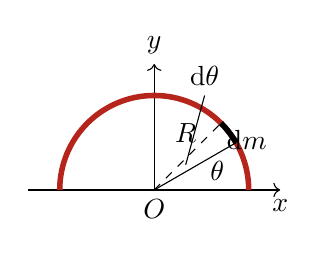
\begin{tikzpicture}[scale=0.8]
            \coordinate[label=below:$x$] (x) at (2,0);
            \coordinate[label=above:$y$] (y) at (0,2);
            \coordinate[label=below:$O$] (O) at (0,0);
            \draw[->] (O) -- (y);
            \draw[->] (-2,0) -- (x);
            \draw[BrickRed, line width=2pt] (1.5,0) arc (0:180:1.5);
            \draw[Black, line width=2pt] (0.75*1.732,0.75) arc (30:45:1.5);
            \draw[dashed] (O) -- (0.75*1.414,0.75*1.414);
            \draw (O) -- (0.75*1.732,0.75);
            \coordinate[label=above:$\theta$] (theta) at (1,0);
            \coordinate[label=above:$R$] (R) at (0.5,0.6);
            \coordinate[label=above:$\rmd \theta$] (dtheta) at (0.8,1.5);
            \draw (0.5,0.4) -- (dtheta);
            \coordinate[label=right:$\rmd m$] (dm) at (1,0.8);
        \end{tikzpicture}
    \]

    \end{exercise}

    \textbf{Solution}
    \vspace{1em}

    建坐标系如图,取一小段长度\(\rmd l\)则其质量为\(\rmd m = \lambda \rmd l\)。

    又\(\rmd l = R \rmd \theta\),故\(\rmd m = \frac{M}{\uppi R} R \rmd \theta\)

    而\(x = R\cos \theta\),\(y = R\sin \theta\)

    故

    $$
        y_c=\frac{\int y \mathrm{~d} m}{M}=\frac{\int_0^\pi R \sin \theta \frac{M}{\pi R} R \mathrm{~d} \theta}{M}=\frac{2 R}{\pi}
    $$

    由对称性可知,

    $$
        x_c = 0
    $$

\chapterimage{miku2.jpg} % Chapter heading image
\chapterspaceabove{6.25cm} % Whitespace from the top of the page to the chapter title on chapter pages
\chapterspacebelow{7.5cm} % Amount of vertical whitespace from the top margin to the start of the text on chapter pages

\chapter{刚体力学}

\section{刚体的定轴转动}

\subsection{刚体}


    \begin{definition}[刚体]
    在外力作用下,形状和大小都不发生变化的物体。(任意两质点间距离保持不变的特殊质点组。)
    \end{definition}

    \begin{enumerate}
        \item 刚体是理想模型;
        \item 刚体模型是为简化研究问题而引进的。
    \end{enumerate}

    \vspace{1em}
    \begin{definition}[平动]
    刚体中所有点的运动轨迹都保持完全相同。(各点的状态一样)

    刚体上任意一点的运动可以代表整个刚体的运动。(刚体平动的运动规律和与质点的运动规律相同)
    \end{definition}

\subsection{转动}

    分为\textbf{定轴转动}和\textbf{非定轴转动}。

    刚体的一般运动可以看作“随质心的平动”和“绕质心的转动”的合成。

\subsubsection{刚体转动的角速度和角加速度}

    \begin{wrapfigure}{r}{4cm}
        \centering
        \includegraphics[scale=0.15]{"Chapter 04 images/pic1.png"}
        % \caption{}
        \label{pic4-1}
    \end{wrapfigure}

    角坐标\(\theta = \theta\left(t\right)\),沿逆时针方向转动为\(\theta > 0\),
    角位移\(\Delta \theta = \theta \left(t + \Delta t\right) - \theta\left(t\right)\)。
    角速度矢量

    \begin{equation}
        \omega=\lim _{\Delta t \rightarrow 0} \frac{\Delta \theta}{\Delta t}=\frac{\mathrm{d} \theta}{\mathrm{~d} t}
    \end{equation}

    方向按右手螺旋法则确定。

\subsubsection{刚体定轴转动}

    刚体定轴转动(一维转动)的转动方向可以用角速度的正、负来表示。

    角加速度

    $$
        \overrightarrow{\alpha} = \deriv{\overrightarrow{\omega}}{t}
    $$

    定轴转动的特点:

    \begin{enumerate}
        \item 每一质点均做圆周运动,与轴垂直的圆面为转动平面;
        \item 任意质点运动\(\Delta \theta,\; \omega,\; \overrightarrow{\omega},\; \overrightarrow{\alpha}\)相同,但\(\overrightarrow{v},\; \overrightarrow{a}\)不相同;
        \item 运动描述仅需一个坐标。
    \end{enumerate}

    匀变速转动公式:

    $$
    \begin{array}{|l|l|}
    \hline \text { 质点匀变速直线运动 } & \text { 刚体绕定轴匀变速转动 } \\
    \hline v=v_0+a t & \omega=\omega_0+\alpha t \\
    \hline x=x_0+v_0 t+\frac{1}{2} a t^2 & \theta=\theta_0+\omega_0 t+\frac{1}{2} \alpha t^2 \\
    \hline v^2=v_0^2+2 a\left(x-x_0\right) & \omega^2=\omega_0^2+2 \alpha\left(\theta-\theta_0\right) \\
    \hline
    \end{array}
    $$

    角量与线量的关系:

    \begin{wrapfigure}{r}{4cm}
        \centering
        \includegraphics[scale=0.2]{"Chapter 04 images/pic2.png"}
        % \caption{}
        \label{pic4-2}
    \end{wrapfigure}

    \[
        \omega = \deriv{\theta}{t}
    \]

    \[
        \overrightarrow{v_i} = r_i \omega \overrightarrow{e}_t
    \]

    $$
        \overrightarrow{v}=\overrightarrow{\omega} \times \overrightarrow{r}_{\perp}=
        \overrightarrow{\omega} \times \overrightarrow{r}
    $$

    $$
        \alpha=\deriv{\omega}{t}=\frac{\rmd^2 \theta}{\rmd^2 t}
    $$

    于是

    \begin{equation}
        \overrightarrow{a}=r \alpha \overrightarrow{e}_{\mathrm{t}}+r \omega^2 \overrightarrow{e}_{\mathrm{n}}
    \end{equation}

\subsection{力矩}

    \begin{definition}[力矩]
    用来描述力对刚体的转动的作用的物理量。
    \end{definition}

    \begin{wrapfigure}{r}{4cm}
        \centering
        \includegraphics[scale=0.2]{"Chapter 04 images/pic3.png"}
        % \caption{}
        \label{pic4-3}
    \end{wrapfigure}

    刚体绕\(Oz\)轴旋转 , 力作用在刚体上点\(P\),且在转动平面内,为由点\(O\)到力的作用点\(P\)的径矢。
    \(\overrightarrow{F}\)对转轴\(z\)的力矩的定义:

    \begin{align}
        \overrightarrow{M} = \overrightarrow{r} \times \overrightarrow{F}
    \end{align}

    $$
        M = Fr\sin\theta = Fd \quad (d\text{为力臂})
    $$

    \begin{enumerate}
        \item 若力\(\overrightarrow{F}\)不在转动平面内,可将力分解为平行和垂直于转轴方向的两个分量;
        \item 合力矩等于各分力矩的矢量和;
        \item 刚体内作用力和反作用力的力矩相互抵消;
        \item 力矩的单位只能用\(\text{牛顿} \cdot \text{米}\),而不能用焦耳。
    \end{enumerate}

\section{转动定律、转动惯量}

\subsection{质点的转动惯量}

    单个质点\(m\)与转轴刚性连接

    \begin{wrapfigure}{r}{4cm}
        \centering
        \includegraphics[scale=0.2]{"Chapter 04 images/pic4.png"}
        % \caption{}
        \label{pic4-4}
    \end{wrapfigure}

    $$
        F_{\mathrm{t}}=m a_{\mathrm{t}}=m r \alpha
    $$

    则

    \begin{equation}
        F_{\mathrm{t}}=m a_{\mathrm{t}}=m r \alpha
    \end{equation}

    \textbf{定义}

    \begin{align}
        I = mr^2
    \end{align}

    为质点\(m\)对\(O\)点的“转动惯量”。

    于是

    \begin{align}
        M = I \alpha
    \end{align}

\subsection{刚体的转动惯量}

    \begin{wrapfigure}{r}{4cm}
        \centering
        \includegraphics[scale=0.2]{"Chapter 04 images/pic5.png"}
        % \caption{}
        \label{pic4-5}
    \end{wrapfigure}

    质量元受外力\(\overrightarrow{F}_{\mathrm{e}j}\),内力\(\overrightarrow{F}_{\mathrm{i}j}\)

    则

    \begin{align*}
        M_{\mathrm{e} j}+M_{\mathrm{i} j}=\Delta m_j r_j^2 \alpha
    \end{align*}

    因为$M_{i j}=-M_{j i}$,所以

    $$
        \sum_j M_{i j}=0
    $$

    于是

    \begin{equation}
        \sum_j M_{\mathrm{e} j}=\left(\sum \Delta m_j r_j^2\right) \alpha
    \end{equation}

    于是\textbf{定义}

    \begin{align}
        I=\sum_j \Delta m_j r_j^2
    \end{align}

    为刚体对\(O\)点的“转动惯量”。

    积分形式即为

    \begin{equation}
        I=\int r^2 \mathrm{~d} m
    \end{equation}

    \begin{wrapfigure}{r}{4cm}
        \centering
        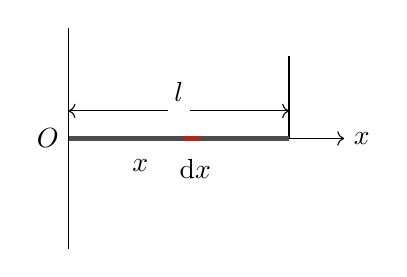
\begin{tikzpicture}[scale=0.7]
            \coordinate[label=left:$O$] (O) at (0,0);
            \coordinate[label=right:$x$] (x_axis) at (5,0);
            \coordinate[label=below:$x$] (x) at (1.3,-0.2);
            \coordinate[label=$l$] (l) at (2,0.5);
            \coordinate[label=below:$\rmd x$] (x) at (2.3,-0.2);
            \draw (0,-2) -- (0,2);
            \draw[->] (O) -- (x_axis);
            \draw (4,0) -- (4,1.5);
            \draw[->] (1.8,0.5) -- (0,0.5);
            \draw[->] (2.2,0.5) -- (4,0.5);
            \draw[line width=2pt, color=black!70] (O) -- (4,0);
            \draw[line width=2pt, color=BrickRed] (2.1,0) -- (2.4,0);
        \end{tikzpicture}
    \end{wrapfigure}

    \textbf{例1 \quad}均匀杆\(m\)对\(O\)轴(通过杆的端点与杆垂直)的转动惯量:

    运用微积分的思想和方法,

    \begin{align*}
        I_{O} = \int x^2 \rmd m = \int_{0}^{l} x^2 \rmd x \lambda = \frac{\lambda l^3}{3} = \frac{1}{3} m l^2
    \end{align*}
    \vspace{1em}

    \begin{wrapfigure}{r}{4cm}
        \centering
        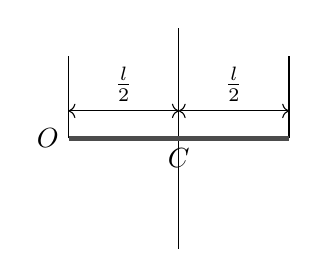
\begin{tikzpicture}[scale=0.7]
            \coordinate[label=left:$O$] (O) at (0,0);
            \coordinate[label=below:$C$] (C) at (2,0);
            \coordinate[label=above:$\frac{l}{2}$] (l-1) at (1,0.5);
            \coordinate[label=above:$\frac{l}{2}$] (l-2) at (3,0.5);
            \draw (O) -- (0,1.5);
            \draw (4,0) -- (4,1.5);
            \draw (2,-2) -- (2,2);
            \draw[<->] (2,0.5) -- (0,0.5);
            \draw[<->] (2,0.5) -- (4,0.5);
            \draw[line width=2pt, color=black!70] (O) -- (4,0);
        \end{tikzpicture}
    \end{wrapfigure}

    \textbf{例2 \quad}均匀杆\(m\)对\(C\)轴(通过杆的端点与杆垂直)的转动惯量:

    $$
        I_C =\frac{1}{12} m l^2
    $$

    \textbf{证}(方法1)

    $$
        \begin{aligned}
            I_C &=\int x^2 \rmd m \\
            &=\int_{-\frac{l}{2}}^{\frac{l}{2}} x^2 d x \lambda\\
            &=\frac{1}{12} \lambda l^3\\
            &=\frac{1}{12} m l^2
        \end{aligned}
    $$

    \textbf{证}(方法2:平行轴定理)

    由平行轴定理,

    $$
        I_O = I_C + m \left(\frac{l}{2}\right)^2
    $$

    于是

    $$
        \begin{aligned}
            I_C &=I_O - m \left(\frac{l}{2}\right)^2 \\
            &=\frac{1}{3} m l^2 - m \left(\frac{l}{2}\right)^2 \\
            &=\frac{1}{12} m l^2
        \end{aligned}
    $$

    \vspace{2em}

    \begin{wrapfigure}{r}{4cm}
        \centering
        \tikzset{every picture/.style={line width=0.75pt}} %set default line width to 0.75pt        
        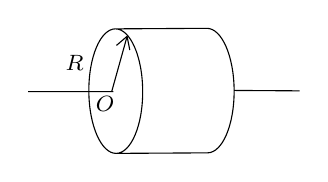
\begin{tikzpicture}[x=0.75pt,y=0.75pt,yscale=-1,xscale=1]
            %uncomment if require: \path (0,300); %set diagram left start at 0, and has height of 300
            %Shape: Can [id:dp17410052803948828] 
            \draw   (167.4,90.33) -- (211.46,90.07) .. controls (218.62,90.03) and (224.5,103.43) .. (224.6,120) ..
                controls (224.69,136.57) and (218.96,150.03) .. (211.8,150.07) -- (167.74,150.33) .. controls
                (160.58,150.37) and (154.7,136.97) .. (154.6,120.4) .. controls (154.51,103.83) and (160.24,90.37) .. (167.4,90.33) ..
                controls (174.56,90.29) and (180.45,103.68) .. (180.54,120.25) .. controls (180.64,136.82) and (174.91,150.29) .. (167.74,150.33) ;
            %Straight Lines [id:da06354151922433426] 
            \draw    (125.4,120.6) -- (166.38,120.54) ;
            %Straight Lines [id:da03453199583434419] 
            \draw    (224.6,120) -- (256.2,120.2) ;
            \draw   (167.91,98.31) -- (173.02,93.94) -- (174.33,100.53) ;
            %Straight Lines [id:da7464924546039589] 
            \draw    (165.62,120.54) -- (173,94.08) ;
            % Text Node
            \draw (156.77,121.4) node [anchor=north west][inner sep=0.75pt]  [font=\footnotesize]  {$O$};
            % Text Node
            \draw (142.15,101.63) node [anchor=north west][inner sep=0.75pt]  [font=\footnotesize]  {$R$};
        \end{tikzpicture}
    \end{wrapfigure}

    \textbf{例3 \quad}均匀圆柱\(m\)对转轴(圆柱体的轴线)的转动惯量:

    $$
        I = \frac{1}{2} m R^2
    $$
    \vspace{2em}

    \begin{wrapfigure}{r}{4cm}
        \centering
        \tikzset{every picture/.style={line width=0.75pt}} %set default line width to 0.75pt        
        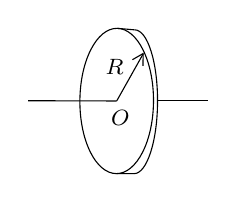
\begin{tikzpicture}[x=0.75pt,y=0.75pt,yscale=-1,xscale=1]
        %uncomment if require: \path (0,300); %set diagram left start at 0, and has height of 300
        %Shape: Ellipse [id:dp023285849196069686] 
        \draw   (169.6,97.35) .. controls (159.81,97.3) and (151.94,81.59) .. (152.04,62.26)
            .. controls (152.13,42.93) and (160.15,27.3) .. (169.94,27.35) .. controls (179.73,27.39) and (187.59,43.1)
            .. (187.5,62.43) .. controls (187.41,81.76) and (179.39,97.39) .. (169.6,97.35) -- cycle ;
        %Shape: Arc [id:dp152216816696912] 
        \draw  [draw opacity=0] (178.39,28.08) .. controls (178.41,28.08) and (178.43,28.08) ..
            (178.45,28.08) .. controls (184.62,28.11) and (189.55,43.64) .. (189.45,62.78) .. controls
            (189.36,81.88) and (184.3,97.35) .. (178.14,97.37) -- (178.28,62.72) -- cycle ;
        \draw (178.39,28.08) .. controls (178.41,28.08) and (178.43,28.08) .. (178.45,28.08) ..
            controls (184.62,28.11) and (189.55,43.64) .. (189.45,62.78) .. controls (189.36,81.88) and (184.3,97.35) .. (178.14,97.37) ;  
        %Straight Lines [id:da15998039992585622] 
        \draw    (169.94,27.35) -- (178.39,28.08) ;
        %Straight Lines [id:da9421417261902603] 
        \draw    (169.6,97.35) -- (178.14,97.37) ;
        %Straight Lines [id:da023543911373016257] 
        \draw    (127.15,62.23) -- (169.77,62.35) ;
        %Straight Lines [id:da05591836369536707] 
        \draw    (189.77,62.23) -- (213.77,62.23) ;
        %Straight Lines [id:da23564039281617188] 
        \draw    (169.77,62.35) -- (182.54,39.62) ;
        \draw   (177.34,42.47) -- (182.49,39.5) -- (182.45,45.45) ;
        % Text Node
        \draw (163.23,41.28) node [anchor=north west][inner sep=0.75pt]  [font=\footnotesize]  {$R$};
        % Text Node
        \draw (165.85,65.74) node [anchor=north west][inner sep=0.75pt]  [font=\footnotesize]  {$O$};
        \end{tikzpicture}
    \end{wrapfigure}

    \textbf{例4 \quad}均匀圆盘\(m\)对转轴(通过盘心垂直于盘面)的转动惯量:

    $$
        I = \frac{1}{2} m R^2
    $$

    \textbf{证}(方法1)

    \[
        \tikzset{every picture/.style={line width=0.75pt}} %set default line width to 0.75pt        
        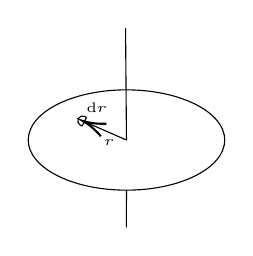
\begin{tikzpicture}[x=0.75pt,y=0.75pt,yscale=-1,xscale=1]
        %uncomment if require: \path (0,300); %set diagram left start at 0, and has height of 300
        %Shape: Ellipse [id:dp6022616866424968] 
        \draw   (213,137.17) .. controls (213,123.82) and (234.19,113) .. (260.33,113) .. controls (286.47,113) and (307.67,123.82) .. (307.67,137.17) .. 
            controls (307.67,150.51) and (286.47,161.33) .. (260.33,161.33) .. controls (234.19,161.33) and (213,150.51) .. (213,137.17) -- cycle ;
        %Straight Lines [id:da33799420686761406] 
        \draw    (260.33,137.17) -- (259.89,83.31) ;
        %Straight Lines [id:da8541013949511429] 
        \draw    (260.29,179.31) -- (260.33,161.33) ;
        %Straight Lines [id:da3324794336188084] 
        \draw    (260.33,137.17) -- (241.12,128.77) ;
        \draw [shift={(239.29,127.96)}, rotate = 23.62] [color={rgb, 255:red, 0; green, 0; blue, 0 }  ][line width=0.75]
            (10.93,-3.29) .. controls (6.95,-1.4) and (3.31,-0.3) .. (0,0) .. controls (3.31,0.3) and (6.95,1.4) .. (10.93,3.29)   ;
        %Shape: Chord [id:dp96440595365312] 
        \draw   (238.98,130.36) .. controls (238.71,130.32) and (238.44,130.24) .. (238.18,130.11) .. controls (236.97,129.48) and (236.48,128.01)
            .. (237.09,126.83) .. controls (237.7,125.65) and (239.18,125.2) .. (240.39,125.82) .. controls (240.65,125.96) and (240.87,126.13) .. (241.06,126.33) -- cycle ;
        % Text Node
        \draw (239.86,117.95) node [anchor=north west][inner sep=0.75pt]  [font=\tiny]  {$\mathrm{d} r$};
        \draw (248.36,135.7) node [anchor=north west][inner sep=0.75pt]  [font=\tiny]  {$r$};
        \end{tikzpicture}
    \]

    设圆盘的面密度为\(\sigma\),则\(\sigma = \dfrac{m}{\uppi R^2}\)

    如图,取微元\(\rmd m\):

    \[
        \tikzset{every picture/.style={line width=0.75pt}} %set default line width to 0.75pt        
        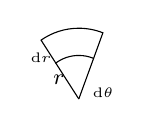
\begin{tikzpicture}[x=0.75pt,y=0.75pt,yscale=-1,xscale=1]
        %uncomment if require: \path (0,300); %set diagram left start at 0, and has height of 300
        %Shape: Block Arc [id:dp4642247634663095] 
        \draw   (206.87,95.84) .. controls (212.07,92.22) and (218.33,90.11) .. (225.06,90.11) .. controls (229.14,90.11) and (233.06,90.89)
            .. (236.66,92.31) -- (232.18,104.64) .. controls (229.97,103.72) and (227.57,103.22) .. (225.06,103.22) .. controls (220.94,103.22)
            and (217.11,104.57) .. (213.95,106.88) -- cycle ;
        %Straight Lines [id:da4857653535391253] 
        \draw    (232.18,104.64) -- (225.06,124.2) ;
        %Straight Lines [id:da18026998140759942] 
        \draw    (213.95,106.88) -- (225.06,124.2) ;
        % Text Node
        \draw (211.49,111.51) node [anchor=north west][inner sep=0.75pt]  [font=\footnotesize]  {$r$};
        \draw (200.69,100.71) node [anchor=north west][inner sep=0.75pt]  [font=\tiny]  {$\mathrm{d} r$};
        \draw (230.62,117.82) node [anchor=north west][inner sep=0.75pt]  [font=\tiny]  {$\mathrm{d} \theta $};
        \end{tikzpicture}
    \]

    则

    \[
        \rmd m = \sigma r \rmd \theta \rmd r
    \]

    于是

    $$
        \begin{aligned}
            I & =\int r^2 \rmd m\\
            & =\int r^2 \sigma r \rmd \theta \rmd r \\
            & =\iint \sigma r^3 \rmd r \rmd \theta \\
            & =\sigma \int_0^R r^3 \rmd r \int_0^{2 \uppi} \rmd \theta \\
            & =\sigma \frac{1}{4} R^4 \cdot 2 \uppi \\
            & =\frac{1}{2} m R^2
        \end{aligned}
    $$

    \textbf{证}(方法2)

    \[
        \tikzset{every picture/.style={line width=0.75pt}} %set default line width to 0.75pt        
        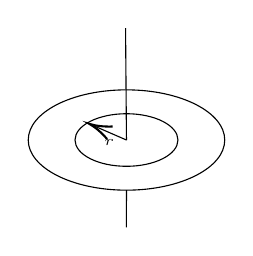
\begin{tikzpicture}[x=0.75pt,y=0.75pt,yscale=-1,xscale=1]
        %uncomment if require: \path (0,300); %set diagram left start at 0, and has height of 300
        %Shape: Ellipse [id:dp6022616866424968] 
        \draw   (213,137.17) .. controls (213,123.82) and (234.19,113) .. (260.33,113) .. controls (286.47,113) and (307.67,123.82)
            .. (307.67,137.17) .. controls (307.67,150.51) and (286.47,161.33) .. (260.33,161.33) .. controls (234.19,161.33) and (213,150.51) .. (213,137.17) -- cycle ;
        %Straight Lines [id:da33799420686761406] 
        \draw    (260.33,137.17) -- (259.89,83.31) ;
        %Straight Lines [id:da8541013949511429] 
        \draw    (260.29,179.31) -- (260.33,161.33) ;
        %Straight Lines [id:da3324794336188084] 
        \draw    (260.33,137.17) -- (244.12,130.12) ;
        \draw [shift={(242.29,129.32)}, rotate = 23.49] [color={rgb, 255:red, 0; green, 0; blue, 0 }  ][line width=0.75] (10.93,-3.29) .. controls
            (6.95,-1.4) and (3.31,-0.3) .. (0,0) .. controls (3.31,0.3) and (6.95,1.4) .. (10.93,3.29)   ;
        %Shape: Ellipse [id:dp4379584317489489] 
        \draw   (235.53,137.17) .. controls (235.53,130.17) and (246.64,124.5) .. (260.33,124.5) .. controls (274.03,124.5) and
            (285.13,130.17) .. (285.13,137.17) .. controls (285.13,144.16) and (274.03,149.83) .. (260.33,149.83) .. controls (246.64,149.83) and (235.53,144.16) .. (235.53,137.17) -- cycle ;
        % Text Node
        \draw (248.36,135.7) node [anchor=north west][inner sep=0.75pt]  [font=\tiny]  {$r$};
        \end{tikzpicture}
    \]

    同样,设圆盘的面密度为\(\sigma = \dfrac{m}{\uppi R^2}\)。取距离圆心\(r\)的某一圆环
    (宽\(\rmd r\))为\(\rmd m\),则

    \[
        \rmd m = \sigma 2 \uppi r \rmd r
    \]

    于是

    $$
        \begin{aligned}
            I &= \int r^2 \rmd m \\
            &= \int_{0}^{R} r^2 \cdot \sigma 2 \uppi r \rmd r \\
            & =\frac{1}{2} m R^2
        \end{aligned}
    $$

    \begin{wrapfigure}{r}{4cm}
        \centering
        \tikzset{every picture/.style={line width=0.75pt}} %set default line width to 0.75pt        
        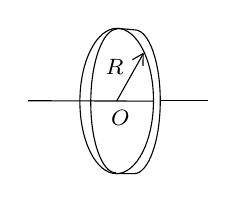
\begin{tikzpicture}[x=0.75pt,y=0.75pt,yscale=-1,xscale=1]
        %uncomment if require: \path (0,300); %set diagram left start at 0, and has height of 300
        %Shape: Ellipse [id:dp023285849196069686] 
        \draw   (169.6,97.35) .. controls (159.81,97.3) and (151.94,81.59) .. (152.04,62.26) ..
            controls (152.13,42.93) and (160.15,27.3) .. (169.94,27.35) .. controls (179.73,27.39) and (187.59,43.1)
            .. (187.5,62.43) .. controls (187.41,81.76) and (179.39,97.39) .. (169.6,97.35) -- cycle ;
        %Shape: Arc [id:dp152216816696912] 
        \draw  [draw opacity=0] (178.39,28.08) .. controls (178.41,28.08) and (178.43,28.08) .. (178.45,28.08)
            .. controls (185.34,28.11) and (190.86,43.65) .. (190.76,62.78) .. controls (190.67,81.89) and (185.02,97.36)
            .. (178.14,97.37) -- (178.28,62.72) -- cycle ; \draw   (178.39,28.08) .. controls (178.41,28.08) and (178.43,28.08)
            .. (178.45,28.08) .. controls (185.34,28.11) and (190.86,43.65) .. (190.76,62.78) .. controls (190.67,81.89) and (185.02,97.36) .. (178.14,97.37) ;  
        %Straight Lines [id:da15998039992585622] 
        \draw    (169.94,27.35) -- (178.39,28.08) ;
        %Straight Lines [id:da9421417261902603] 
        \draw    (169.6,97.35) -- (178.14,97.37) ;
        %Straight Lines [id:da023543911373016257] 
        \draw    (127.15,62.23) -- (187.5,62.43) ;
        %Straight Lines [id:da05591836369536707] 
        \draw    (191.31,62.23) -- (213.77,62.23) ;
        %Straight Lines [id:da23564039281617188] 
        \draw    (169.77,62.35) -- (182.54,39.62) ;
        \draw   (177.34,42.47) -- (182.49,39.5) -- (182.45,45.45) ;
        %Shape: Arc [id:dp47532243106850425] 
        \draw  [draw opacity=0] (169.5,96.99) .. controls (169.48,96.99) and (169.46,96.99) ..
            (169.44,96.99) .. controls (162.54,96.93) and (157.1,81.36) .. (157.28,62.23) .. controls (157.47,43.12)
            and (163.19,27.68) .. (170.07,27.7) -- (169.77,62.35) -- cycle ; \draw   (169.5,96.99) ..
            controls (169.48,96.99) and (169.46,96.99) .. (169.44,96.99) .. controls (162.54,96.93) and (157.1,81.36)
            .. (157.28,62.23) .. controls (157.47,43.12) and (163.19,27.68) .. (170.07,27.7) ;  
        % Text Node
        \draw (163.23,41.28) node [anchor=north west][inner sep=0.75pt]  [font=\footnotesize]  {$R$};
        % Text Node
        \draw (165.85,65.74) node [anchor=north west][inner sep=0.75pt]  [font=\footnotesize]  {$O$};
        \end{tikzpicture}
    \end{wrapfigure}

    \textbf{例5 \quad}均匀圆环\(m\)对转轴(通过环心垂直于盘面)的转动惯量:

    $$
        I = m R^2
    $$
    \vspace{2em}

    \begin{wrapfigure}{r}{4cm}
        \centering
        \tikzset{every picture/.style={line width=0.75pt}} %set default line width to 0.75pt        
        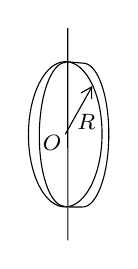
\begin{tikzpicture}[x=0.75pt,y=0.75pt,yscale=-1,xscale=1]
        %uncomment if require: \path (0,300); %set diagram left start at 0, and has height of 300
        %Shape: Ellipse [id:dp023285849196069686] 
        \draw   (169.6,97.35) .. controls (159.81,97.3) and (151.94,81.59) .. (152.04,62.26)
            .. controls (152.13,42.93) and (160.15,27.3) .. (169.94,27.35) .. controls (179.73,27.39) and (187.59,43.1)
            .. (187.5,62.43) .. controls (187.41,81.76) and (179.39,97.39) .. (169.6,97.35) -- cycle ;
        %Shape: Arc [id:dp152216816696912] 
        \draw  [draw opacity=0] (178.39,28.08) .. controls (178.41,28.08) and (178.43,28.08) .. (178.45,28.08) ..
            controls (185.34,28.11) and (190.86,43.65) .. (190.76,62.78) .. controls (190.67,81.89) and (185.02,97.36)
            .. (178.14,97.37) -- (178.28,62.72) -- cycle ; \draw   (178.39,28.08) .. controls (178.41,28.08) and (178.43,28.08)
            .. (178.45,28.08) .. controls (185.34,28.11) and (190.86,43.65) .. (190.76,62.78) .. controls (190.67,81.89)
            and (185.02,97.36) .. (178.14,97.37) ;  
        %Straight Lines [id:da15998039992585622] 
        \draw    (169.94,27.35) -- (178.39,28.08) ;
        %Straight Lines [id:da9421417261902603] 
        \draw    (169.6,97.35) -- (178.14,97.37) ;
        %Straight Lines [id:da23564039281617188] 
        \draw    (169.77,62.35) -- (182.54,39.62) ;
        \draw   (177.34,42.47) -- (182.49,39.5) -- (182.45,45.45) ;
        %Shape: Arc [id:dp47532243106850425] 
        \draw  [draw opacity=0] (169.5,96.99) .. controls (169.48,96.99) and (169.46,96.99) ..
            (169.44,96.99) .. controls (162.54,96.93) and (157.1,81.36) .. (157.28,62.23) ..
            controls (157.47,43.12) and (163.19,27.68) .. (170.07,27.7) -- (169.77,62.35) -- cycle ;
        \draw (169.5,96.99) .. controls (169.48,96.99) and (169.46,96.99) .. (169.44,96.99) ..
            controls (162.54,96.93) and (157.1,81.36) .. (157.28,62.23) .. controls (157.47,43.12) and (163.19,27.68) .. (170.07,27.7) ;  
        %Straight Lines [id:da7330715455990151] 
        \draw    (170.96,11.25) -- (171.04,113.44) ;
        % Text Node
        \draw (174.31,51.43) node [anchor=north west][inner sep=0.75pt]  [font=\footnotesize]  {$R$};
        % Text Node
        \draw (157.69,61.74) node [anchor=north west][inner sep=0.75pt]  [font=\footnotesize]  {$O$};
        \end{tikzpicture}
    \end{wrapfigure}

    \textbf{例6 \quad}均匀圆环\(m\)对转轴(沿圆环直径)的转动惯量:

    $$
        I = \frac{1}{2} m R^2
    $$
    \vspace{4em}

    \begin{wrapfigure}{r}{4cm}
        \centering
        \tikzset{every picture/.style={line width=0.75pt}} %set default line width to 0.75pt        
        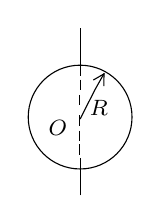
\begin{tikzpicture}[x=0.75pt,y=0.75pt,yscale=-1,xscale=1]
        %uncomment if require: \path (0,300); %set diagram left start at 0, and has height of 300
        %Straight Lines [id:da23564039281617188] 
        \draw    (171,61.56) -- (178.11,47.51) -- (182.54,39.62) ;
        \draw   (177.34,42.77) -- (182.49,39.81) -- (182.45,45.76) ;
        %Straight Lines [id:da7330715455990151] 
        \draw    (171,17.81) -- (171,35.62) ;
        %Shape: Circle [id:dp7000744143017317] 
        \draw   (146,60.62) .. controls (146,46.81) and (157.19,35.62) ..
            (171,35.62) .. controls (184.81,35.62) and (196,46.81) .. (196,60.62) .. controls
            (196,74.42) and (184.81,85.62) .. (171,85.62) .. controls (157.19,85.62)
            and (146,74.42) .. (146,60.62) -- cycle ;
        %Straight Lines [id:da5423143354957887] 
        \draw    (171,98.31) -- (171,85.62) ;
        %Straight Lines [id:da1925163091022266] 
        \draw    (171,35.62) -- (171,40.69) ;
        %Straight Lines [id:da49186666744211105] 
        \draw    (171,42.62) -- (171,47.69) ;
        %Straight Lines [id:da6273845348478542] 
        \draw    (170.88,49.87) -- (170.88,54.94) ;
        %Straight Lines [id:da5600475408875403] 
        \draw    (170.63,59.62) -- (170.63,64.69) ;
        %Straight Lines [id:da3768869837055404] 
        \draw    (170.75,67.12) -- (170.75,72.19) ;
        %Straight Lines [id:da21244422124496465] 
        \draw    (170.88,73.62) -- (170.88,78.69) ;
        %Straight Lines [id:da19418219961056882] 
        \draw    (171,80.54) -- (171,85.62) ;
        % Text Node
        \draw (174.46,51.43) node [anchor=north west][inner sep=0.75pt]  [font=\footnotesize]  {$R$};
        % Text Node
        \draw (154.6,60.92) node [anchor=north west][inner sep=0.75pt]  [font=\footnotesize]  {$O$};
        \end{tikzpicture}
    \end{wrapfigure}

    \textbf{例7 \quad}薄球壳\(m\)对转轴(沿直径)的转动惯量:

    $$
        I = \frac{2}{3} m R^2
    $$
    \vspace{4em}

    \begin{wrapfigure}{r}{4cm}
        \centering
        \tikzset{every picture/.style={line width=0.75pt}} %set default line width to 0.75pt        
        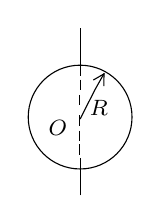
\begin{tikzpicture}[x=0.75pt,y=0.75pt,yscale=-1,xscale=1]
        %uncomment if require: \path (0,300); %set diagram left start at 0, and has height of 300
        %Straight Lines [id:da23564039281617188] 
        \draw (171,61.56) -- (178.11,47.51) -- (182.54,39.62) ;
        \draw (177.34,42.77) -- (182.49,39.81) -- (182.45,45.76) ;
        %Straight Lines [id:da7330715455990151] 
        \draw (171,17.81) -- (171,35.62) ;
        %Shape: Circle [id:dp7000744143017317] 
        \draw (146,60.62) .. controls (146,46.81) and (157.19,35.62) ..
            (171,35.62) .. controls (184.81,35.62) and (196,46.81) .. (196,60.62) .. controls
            (196,74.42) and (184.81,85.62) .. (171,85.62) .. controls (157.19,85.62)
            and (146,74.42) .. (146,60.62) -- cycle ;
        %Straight Lines [id:da5423143354957887] 
        \draw (171,98.31) -- (171,85.62) ;
        %Straight Lines [id:da1925163091022266] 
        \draw (171,35.62) -- (171,40.69) ;
        %Straight Lines [id:da49186666744211105] 
        \draw (171,42.62) -- (171,47.69) ;
        %Straight Lines [id:da6273845348478542] 
        \draw (170.88,49.87) -- (170.88,54.94) ;
        %Straight Lines [id:da5600475408875403] 
        \draw (170.63,59.62) -- (170.63,64.69) ;
        %Straight Lines [id:da3768869837055404] 
        \draw (170.75,67.12) -- (170.75,72.19) ;
        %Straight Lines [id:da21244422124496465] 
        \draw (170.88,73.62) -- (170.88,78.69) ;
        %Straight Lines [id:da19418219961056882] 
        \draw (171,80.54) -- (171,85.62) ;
        % Text Node
        \draw (174.46,51.43) node [anchor=north west][inner sep=0.75pt]  [font=\footnotesize]  {$R$};
        % Text Node
        \draw (154.6,60.92) node [anchor=north west][inner sep=0.75pt]  [font=\footnotesize]  {$O$};
        \end{tikzpicture}
    \end{wrapfigure}

    \textbf{例8 \quad}均匀实心球体\(m\)对转轴(沿直径)的转动惯量:

    $$
        I = \frac{2}{5} m R^2
    $$
    \vspace{2em}

\subsection{转动定律}

\begin{theorem}[转动定律]
    \begin{align}
        M = I \alpha
    \end{align}
\end{theorem}

    \begin{enumerate}
        \item 若\(M=0\),则\(\alpha=0\),即\(\omega\)不变;
        \item \(\alpha \)与\(\dfrac{M}{I}\)成反比;
        \item \(M = I\alpha = I\dderiv{\omega}{t}\);
        \item 转动惯量的单位为\(\mathrm{kg} \cdot \mathrm{m^2}\);
        \item 转动惯量的是对某一转轴而言的;
        \item 转动惯量是转动惯性的量度;
        \item 转动惯量具有可叠加性;
        \item 转动惯量与刚体的质量、质量的分布以及转轴的位置有关。
    \end{enumerate}

    \begin{wrapfigure}{r}{4cm}
        \centering
        \includegraphics[scale=0.2]{"Chapter 04 images/pic6.png"}
        % \caption{}
        \label{pic4-6}
    \end{wrapfigure}

\begin{theorem}[平行轴定理]
    质量为\(m\)的刚体,如果对其质心轴的转动惯量为\(I_{C}\),则对任一与该轴平行,
    相对\(d\)的转轴的转动惯量

    \begin{align}
        I = I_{C} + md^2
    \end{align}
\end{theorem}

\begin{theorem}[垂直轴定理(正交轴定理)]

    对\textbf{薄板状}刚体:对板面内相互垂直的两个定轴的转动惯量之和
    等于该刚体对通过两轴交点且垂直于板面的定轴的转动惯量。

    \begin{align}
        I_{z} = I_{x} + I_{y}
    \end{align}
\end{theorem}

    证明:

    \begin{align*}
        \begin{aligned}
            I_{z} &= \sum \Delta m_{i}r_{i}^2 \\
            &= \sum \Delta m_{i}\left(x_{i}^2 + y_{i}^2\right) \\
            &= I_{x} + I_{y}
        \end{aligned}
    \end{align*}

\subsection{例题}

\begin{exercise}
    质量为\(M\)的匀质圆盘,可绕通过盘中心并垂直于盘面的固定光滑轴转动,转动惯量为
    \(\frac{1}{2}Mr^2\)。一根长为\(l\),质量为\(m\)的匀质柔软绳索挂在圆盘上,如图所示。
    设绳与圆盘间无相对滑动,试求当圆盘两侧绳长之差为\(S\)时,绳的加速度的大小。
    \vspace{1em}
\end{exercise}

    \begin{wrapfigure}{r}{4cm}
        \centering
        \includegraphics[scale=0.2]{"Chapter 04 images/pic7.png"}
        % \caption{}
        \label{pic4-7}
    \end{wrapfigure}

    \textbf{Solution}
    \vspace{1em}

    设某一时刻圆盘两侧的绳长分别为\(x_1\)、\(x_2\)(\(x_1 > x_2\)),如图所示。
    可将绳分为三段,即长度分别为\(x1\)、\(x2\)的两段绳和绕在盘上的一段,
    由于绕在盘上的一段谁盘一起转动,所以可将它和盘作为一个整体来讨论。
    假设在 1、2 两点处绳中的张力分别为\(T_1\)、\(T_2\),则由牛顿定律和转动定律可得

    \[
        x_2 \rho g - T_2 = x_2 \rho a
    \]

    \[
        T_1 - x_1 \rho g = x_1 \rho a
    \]

    \[
        T_2r - T_1r = I \alpha
    \]

    且

    \[
        a = r\alpha
    \]

    式中,

    \[
        \rho = \frac{m}{l}
    \]

    是绳的线密度,

    \[
        I = \frac{1}{2}Mr^2 + \uppi r \rho \cdot r^2
    \]

    是绕在盘上的绳与盘作为整体的转动惯量。

    联立以上方程,并取\(x_2-x_1=S\),可得绳的加速度为

    $$
        a=\frac{2 m g S}{(2 m+M) l}
    $$

\section{刚体定轴转动的功能关系}

\subsection{力矩做功}

    \(\overrightarrow{F}\)在转动平面内,

    \begin{equation*}
        \mathrm{d} A=\overrightarrow{F} \cdot \mathrm{~d} \overrightarrow{r}=F_\tau \mathrm{d} s=F_\tau r \mathrm{~d} \theta
        \label{formula-4-3-1}
    \end{equation*}

    上式也可写成

    \begin{equation}
        \mathrm{d} A = M \rmd \theta
    \end{equation}

    于是力矩\(M\)对刚体所做的总功为

    \begin{equation}
        A=\int \mathrm{d} A=\int_{\theta_0}^\theta M \mathrm{~d} \theta
    \end{equation}

    由式\ref{formula-4-3-1}还可得出力矩做功的瞬时功率为

    \begin{equation}
        P=\frac{\mathrm{d} A}{\mathrm{~d} t}=\frac{M \mathrm{~d} \theta}{\mathrm{~d} t}=M \omega
    \end{equation}

    当\(\overrightarrow{M}\)与\(\overrightarrow{\omega}\)同向,\(W\)、\(P\)为正;
    当\(\overrightarrow{M}\)与\(\overrightarrow{\omega}\)反向,\(W\)、\(P\)为负。

\subsection{转动动能}

    整个刚体的动能就是所有质元的动能之和:

    \begin{equation}
        E_{\mathrm{k}}=\sum_i \frac{1}{2} \Delta m_i r_i^2 \omega^2=\frac{1}{2}\left(\sum_i \Delta m_i r_i^2\right) \omega^2
    \end{equation}

    即

    \begin{equation}
        E_{\mathrm{k}}=\frac{1}{2} I \omega^2
    \end{equation}

\subsection{刚体定轴转动的动能定理}

    由

    \begin{equation*}
        A=\int_{\theta_1}^{\theta_2} M \mathrm{~d} \theta=\int_{\theta_1}^{\theta_2} I \frac{\mathrm{~d} \omega}{\mathrm{~d} t} \mathrm{~d} \theta=\int_{\omega_1}^{\omega_2} I \omega \mathrm{~d} \omega
    \end{equation*}

    有

    \begin{equation}
        A=\int_{\theta_1}^{\theta_2} M \mathrm{~d} \theta=\int_{\omega_1}^{\omega_2} I \omega \mathrm{~d} \omega=\frac{1}{2} I \omega_2^2-\frac{1}{2} I \omega_1^2
    \end{equation}

    即:合外力矩对绕定轴转动的刚体所作的功等于刚体转动动能的增量。
    ——刚体绕定轴转动的动能定理

\section{刚体的角动量、角动量定理、角动量守恒定律}

    \textbf{力}的时间累积效应:冲量、动量、动量定理。

    \textbf{力矩}的时间累积效应:冲量矩、角动量、角动量定理。

\subsection{刚体定轴转动的角动量}

\begin{definition}[质点的角动量]
    质量为\(m\)的质点以速度\(\overrightarrow{v}\)在空间运动,某时刻对\(O\)的位矢为
    \(\overrightarrow{r}\),则质点对\(O\)的角动量定义为

    \begin{equation}
        \overrightarrow{L} = \overrightarrow{r} \times \overrightarrow{p}
        = \overrightarrow{r} \times m \overrightarrow{v}
    \end{equation}

    \[
        \includegraphics[scale=0.12]{"Chapter 04 images/pic8.png"}
        % \caption{}
        \label{pic4-8}
    \]

    当质点以角速度\(\omega\)作半径为\(r\)的圆运动时,
    相对圆心的角动量:

    \begin{equation}
        L = r m v = r^2 m \omega
    \end{equation}
    
    (方向按右手螺旋法则确定)
\end{definition}

\begin{definition}[刚体的角动量]

    对于绕\(z\)轴转动的刚体(质点系,每个质点做圆周运动):

    \begin{equation}
        L_z =\sum_i L_{z i}=\sum_i r_i^2 \Delta m_i \omega
        =\left(\sum_i r_i^2 \Delta m_i\right) \omega=I_z \omega
    \end{equation}
\end{definition}

\subsection{刚体定轴转动的角动量定理}

\begin{theorem}[质点的角动量定理]
    \begin{equation}
        \overrightarrow{M} = \deriv{\overrightarrow{L}}{t}
    \end{equation}

    作用于质点的合外力对参考点0的力矩,等于质点对该点\(O\)的角动量随时间的变化率。

    微分形式:

    \begin{equation}
        \overrightarrow{M} \rmd t = \rmd L
    \end{equation}

    积分形式:

    \begin{equation}
        \int_{t_1}^{t_2} \overrightarrow{M} \rmd t = \overrightarrow{L}_2 - \overrightarrow{L}_1
    \end{equation}
\end{theorem}

    定义\textbf{冲量矩}:

    \begin{equation}
        \int_{t_1}^{t_2} \overrightarrow{M} \rmd t
    \end{equation}

    质点的角动量定理另一表述:对同一参考点\(O\),
    质点所受的冲量矩等于质点角动量的增量。

\begin{theorem}[质点的角动量守恒定律]

    由质点的角动量定理:

    如果\(\overrightarrow{M}=\overrightarrow{0}\),则

    \begin{equation}
        \overrightarrow{L} = \overrightarrow{r} \times m \overrightarrow{v}
        = \text{恒矢量}
    \end{equation}

    若质点所受外力对某给定点\(O\)的力矩为零,则质点对\(O\)点的角动量保持不变。
\end{theorem}

\begin{theorem}[刚体定轴转动的角动量定理]

    刚体也是质点系,刚体定轴转动的角动量定理的微分形式应为

    \begin{equation}
        M \rmd t = \rmd \left(I \omega\right)
    \end{equation}

    \textbf{注意}:这两式对非刚体(转动惯量会发生变化)也成立。

    而刚体绕定轴的转动定律:

    \begin{equation}
        M = I \deriv{\omega}{t}
    \end{equation}

    (\(I\)是常数,仅对刚体成立)

    刚体(非刚体)定轴转动的角动量定理的积分形式:

    \begin{equation}
        \int_{t_1}^{t_2} M \mathrm{~d} t=\int_{\left(I \omega\right)_1}^{\left(I \omega\right)_2} \rmd \left(I \omega\right)
        =I_2 \omega_2-I_1 \omega_1
    \end{equation}
\end{theorem}

\subsection{刚体定轴转动的角动量守恒定律}

    如果\(\overrightarrow{M}=\overrightarrow{0}\),则

    \begin{equation}
        L = I \omega = \text{常量}
    \end{equation}

    若物体所受的合外力矩为零,则物体的角动量保持不变。

    \begin{enumerate}
        \item 若\(I\)不变,\(\omega\)不变;
        \item 若\(I\)变,\(\omega\)也变,但\(L = I \omega\)不变。
    \end{enumerate}

    即内力矩不改变系统的角动量。

    在冲击等问题中,\(M^{\text{in}} \gg  M^{\text{ex}}\),可认为\(L \approx \text{常量}\)。

\subsection{共轴系统定轴转动的角动量定理}

    当一个系统由多个物体和质点组成时,则某段时间内对某轴
    的合外力矩的冲量矩等于系统绕该轴的角动量的增量:

    $$
    \int_{t_1}^{t_2} M \mathrm{~d} t=\left(\sum_i I_i \omega_i\right)_2-\left(\sum I_i \omega_i\right)_1
    $$

    (\(I_i\)、\(\omega_i\)应对同一轴,\(\omega_i\)应对同一惯性系。)

    共轴系统的定轴转动的角动量守恒定律:

    当系统对某轴的合外力矩的冲量矩等于零时,系统绕该轴的角动量守恒,即:

    \begin{equation}
        \int_{t_1}^{t_2} M \rmd t \text{时,} \sum_{i} I_i \omega_i = \text{恒矢量}
    \end{equation}

    (\(I_i\)、\(\omega_i\)应对同一轴,\(\omega_i\)应对同一惯性系。)

\subsection{例题}

\begin{exercise}
    在半径为\(R\)、质量为\(M\)具有光滑竖直固定中心轴的水平圆盘上,
    有一人静止站立在距转轴为\(\frac{R}{2}\)处,人的质量是圆盘质量的\(\frac{1}{10}\),
    开始时载人圆盘对地以角速度\(\omega_0\)匀速转动。现在此人相对于圆盘以速率\(v\)沿与圆盘转动的相反方向绕轴作圆周运动,
    如图所示。已知圆盘对中心轴的转动惯量为\(\frac{1}{2}MR^2\)。试求:

    \begin{enumerate}
        \item 圆盘对地的角速度;
        \item 欲使圆盘对地静止,人在该圆周上相对于圆盘的速度\(v\)的大小及方向。
    \end{enumerate}

    \[
        \includegraphics[scale=0.24]{Chapter 04 images/pic9.png}
    \]
\end{exercise}

    \vspace{1em}
    \textbf{Solution}
    
    \textbf{Part One}

    当人以速率\(v\)沿相对圆盘转动相反的方向走动时,圆盘对地的角速度为\(\omega\),
    则由速度叠加原理可知,人相对于地角速度为

    $$
        \omega^{\prime}=\omega-\frac{v}{R / 2}=\omega-\frac{2 v}{R}
    $$

    将人与盘视为一个共轴系统,人在盘上走动时系统受对转轴的合外力矩为零,
    故系统的角动量守恒,所以有

    $$
        \left[\frac{1}{2} M R^2+\frac{M}{10}\left(\frac{1}{2} R\right)^2\right] \omega_0=
        \frac{1}{2} M R^2 \omega+\frac{M}{10}\left(\frac{1}{2} R\right)^2 \omega^{\prime}
    $$

    联解得

    $$
        \omega=\omega_0+\frac{2 v}{21 R}
    $$

    \textbf{Part Two}

    欲使盘对地静止,则\(\omega=0\)必为零,即
    
    $$
        \omega=\omega_0+\frac{2 v}{21 R}=0
    $$

    由此得,人相对于圆盘的速度为

    $$
        v=-\frac{21 R \omega_0}{2}
    $$

    式中负号表示人的走动方向与上一问中人走动的方向相反,即与盘的初始转动方向一致。
    \vspace{1em}

\begin{exercise}
    一块宽\(L=0.60\mathrm{m}\) 、质量\(M=1.0\mathrm{kg}\)的均匀薄木板,
    可绕水平固定轴\(OO^{\prime}\)无摩擦地自由转动。当木板静止在平衡位置时,有一质量为
    \(m = 10 \times 10^3 \mathrm{kg}\)的子弹垂直击中木板上的\(A\)点,\(A\)离转轴\(OO^{\prime}\)距离
    \(l = 0.36\mathrm{m}\),子弹击中木板前的速度为\(500 m \cdot s^{-1}\),穿出木板后的速度为\(200 m \cdot s^{-1}\)。
    试求

    \begin{enumerate}
        \item 子弹给予木板的冲量;
        \item 木板获得的角速度。
    \end{enumerate}

    (已知:木板绕\(OO^{\prime}\)轴的转动惯量\(I=\frac{1}{3}ML^2\))

    \[
        \includegraphics[scale=0.24]{Chapter 04 images/pic10.png}
    \]
\end{exercise}

    \vspace{1em}
    \textbf{Solution}
    
    \textbf{Part One}

    子弹受到的冲量为

    $$
        I=\int F \mathrm{~d} t=m\left(v-v_0\right)
    $$
    
    由牛顿第三定律,子弹对木块的冲量为

    $$
        I^{\prime}=\int F^{\prime} \mathrm{d} t=-\int F \mathrm{~d} t=m\left(v_0-v\right)=3.0 \mathrm{N \cdot m}
    $$

    \textbf{Part Two}

    若将子弹和木板作为一个共轴系统,则该系统在碰撞过程中满足角动量守恒条件。
    所以有

    $$
        m v_0 l=m v l+I \omega
    $$

    所以木板获得的角速度为

    $$
        \omega=\frac{m v_0 l-m v l}{I}=\frac{3\left(m v_0 l-m v l\right)}{M L^2}
        =9.0 \mathrm{rad} \cdot \mathrm{~s}^{-1}
    $$

\chapterimage{miku3.png} % Chapter heading image
\chapterspaceabove{6.25cm} % Whitespace from the top of the page to the chapter title on chapter pages
\chapterspacebelow{7.5cm} % Amount of vertical whitespace from the top margin to the start of the text on chapter pages

\chapter{机械振动}

\section{简谐振动}

\subsection{简谐振动的动力学特征}

\subsubsection{弹簧振子的振动}

    模型:谐振子轻弹簧(不计质量)与物体(看成质点)

    弹簧振子的无阻尼自由振动:

    \[
        \includegraphics[scale=0.5]{Chapter 06 images/pic1.png}
    \]

    振动的成因:

    \begin{enumerate}
        \item 回复力;
        \item 惯性。
    \end{enumerate}

\subsubsection{弹簧振子的运动方程}

    \begin{equation}
        F=-k x=m a=m \frac{\rmd^2 x}{\rmd t^2}
    \end{equation}

    令
    
    \[
        \omega^2=\frac{k}{m}
    \]
    
    得
    
    \[
        \dfrac{\rmd^2 x}{\rmd t^2} = -\omega^2 x
    \]

    即\(a=-\omega^2 x\)

    具有加速度\(a\)与位移的大小\(x\)成正比,而方向相反特征的振动称为简谐运动。

    简谐运动的微分方程:

    \begin{align}
        \dfrac{\rmd^2 x}{\rmd t^2} = -\omega^2 x
        \label{6-1-2}
    \end{align}

    解得

    \begin{align}
        x = A \cos\left(\omega t + \varphi\right)
    \end{align}

    或

    \begin{align}
        x = A \sin\left(\omega t + \varphi + \frac{\uppi}{2}\right)
    \end{align}

    用复指数表示
    
    \begin{equation}
        x=A \mathrm{e}^{\mathrm{i}(\omega t+\varphi)}
    \end{equation}

    \textbf{公式之间的相互推导关系}

    \[
        \tikzset{every picture/.style={line width=0.75pt}} %set default line width to 0.75pt
        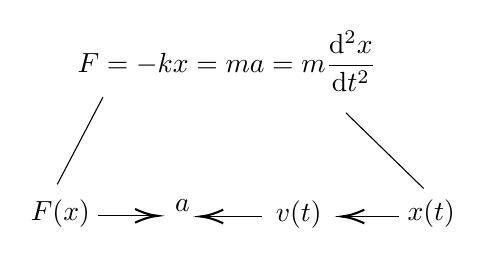
\begin{tikzpicture}[x=0.75pt,y=0.75pt,yscale=-1,xscale=1]
            %uncomment if require: \path (0,300); %set diagram left start at 0, and has height of 300
            %Straight Lines [id:da5445518985427571] 
            \draw    (155.43,153.29) -- (182.43,153.29) ;
            \draw [shift={(184.43,153.29)}, rotate = 180] [color={rgb, 255:red, 0; green, 0; blue, 0 }  ][line width=0.75]
                (10.93,-3.29) .. controls (6.95,-1.4) and (3.31,-0.3) .. (0,0) .. controls (3.31,0.3) and (6.95,1.4) .. (10.93,3.29)   ;
            %Straight Lines [id:da8539578247281134] 
            \draw    (234.5,153.61) -- (207,153.61) ;
            \draw [shift={(205,153.61)}, rotate = 360] [color={rgb, 255:red, 0; green, 0; blue, 0 }  ][line width=0.75]
                (10.93,-3.29) .. controls (6.95,-1.4) and (3.31,-0.3) .. (0,0) .. controls (3.31,0.3) and (6.95,1.4) .. (10.93,3.29)   ;
            %Straight Lines [id:da08053806804260755] 
            \draw    (300.5,153.61) -- (275,153.61) ;
            \draw [shift={(273,153.61)}, rotate = 360] [color={rgb, 255:red, 0; green, 0; blue, 0 }  ][line width=0.75]
                (10.93,-3.29) .. controls (6.95,-1.4) and (3.31,-0.3) .. (0,0) .. controls (3.31,0.3) and (6.95,1.4) .. (10.93,3.29)   ;
            %Straight Lines [id:da2022111052056348] 
            \draw    (158,96.11) -- (136,138.11) ;
            %Straight Lines [id:da9851232959428675] 
            \draw    (275,103.61) -- (312.5,140.11) ;
            % Text Node
            \draw (122,144.4) node [anchor=north west][inner sep=0.75pt]    {$F( x)$};
            \draw (191.5,144.4) node [anchor=north west][inner sep=0.75pt]    {$a$};
            \draw (240,144.9) node [anchor=north west][inner sep=0.75pt]    {$v( t)$};
            \draw (303.5,144.4) node [anchor=north west][inner sep=0.75pt]    {$x( t)$};
            \draw (144.5,62.9) node [anchor=north west][inner sep=0.75pt]    {$F=-kx=ma=m\dfrac{\mathrm{d}^{2} x}{\mathrm{d} t^{2}}$};
        \end{tikzpicture}
    \]

\subsection{谐振动的速度和加速度}

    由

    \begin{align*}
        x = A \cos\left(\omega t + \varphi\right)
    \end{align*}

    运动方程对时间求导

    \begin{equation}
        v=\frac{\mathrm{d} x}{\mathrm{~d} t}=-\omega A \sin (\omega t+\varphi)=-v_{\mathrm{m}} \sin (\omega t+\varphi)
    \end{equation}

    运动方程对时间求二阶导

    \begin{equation}
        a=\frac{\mathrm{d}^2 x}{\mathrm{~d} t^2}=-\omega^2 A \cos (\omega t+\varphi)=
        -a_{\mathrm{m}} \cos (\omega t+\varphi)
    \end{equation}

    其中,

    $$
        A=\sqrt{x_0^2+\left(\frac{v_0}{\omega}\right)^2}
    $$

    $$
        \varphi=\arctan \left(-\frac{v_0}{\omega x_0}\right)
    $$

    (此结果一般有两个值,最后要舍去一个,根据速度的方向。)
    
    \[
        \includegraphics[scale=0.5]{Chapter 06 images/pic2.png}
    \]

\subsection{描述简谐振动的物理量}

    振幅 (amplitude):

    \begin{align}
        x_m = A
    \end{align}

    周期 (period):

    \begin{align}
        T = \frac{2 \uppi}{\omega}
    \end{align}

    简谐运动中,\(\omega\)被称为角频率或圆频率

    \begin{align}
        \omega = \sqrt{\frac{k}{m}}
    \end{align}

    频率 (frequency):

    \begin{align}
        \nu = \frac{1}{T}
    \end{align}

    相位 (phase):

    \begin{align}
        \left(\omega t + \varphi\right)
    \end{align}

    初相位(初相,initial phase)

    \begin{align}
        \varphi
    \end{align}

    相位差:

    设有两个同方向、同频率的简谐振动,它们的振动表达式分别为
    
    $$
        \begin{aligned}
            & x_1=A_1 \cos \left(\omega t+\varphi_1\right) \\
            & x_2=A_2 \cos \left(\omega t+\varphi_2\right)
        \end{aligned}
    $$

    它们在任意时刻的相位差为

    \begin{align}
        \Delta \varphi = \left(\omega t+\varphi_1\right) - \left(\omega t+\varphi_2\right)
    \end{align}

    不同简谐振动在同一时刻,两者的相位之差值
    可以判断它们的步调:超前、落后。

    $$
    \Delta \varphi=\varphi_2-\varphi_1\left\{\begin{array}{l}
        2 k \uppi, \quad \text{同相} \\
        2(k+1) \uppi, \quad \text{反相} \\
        >0, \quad \text{\(x_2\)比\(x_1\)超前(或\(x_1\)比\(x_2\))落后} \\
        < 0, \quad \text{\(x_2\)比\(x_1\)落后(或\(x_1\)比\(x_2\))超前}
        \end{array}\right.
    $$

    注意:超前、落后以\(\left|\Delta \varphi\right| < \uppi\)的相位角来判断。

\subsubsection{解析法描述简谐运动}

    \[
        x = A \cos \left(\omega t + \varphi\right)
    \]

\subsubsection{参考圆表示法}

    \[
        \includegraphics[scale=0.25]{Chapter 06 images/pic3.png}
    \]

    一个动点在参考圆上匀速转动,
    以该动点在参考一个动点在参考圆上匀圆的一根直径上的投影点的运动可代表简谐振动。

    \subsubsection{旋转矢量表示法简谐振动}

    \[
        \includegraphics[scale=0.25]{Chapter 06 images/pic4.png}
    \]

    旋转矢量法:矢量\(\overrightarrow{A}\)的端点在\(x\)轴上投影点的运动规律。
    使相位表示更加直观。

    \[
        \includegraphics[scale=0.25]{Chapter 06 images/pic5.png}
    \]

    \begin{enumerate}
        \item 在平面图上作一\(Ox\)轴;
        \item 振幅矢量\(\overrightarrow{A}\)从初相位置开始绕\(Ox\)轴上\(O\)点以匀角速度\(\omega\)逆时针旋转,转一圈所用的时间\(T\);
        \item 矢量\(\overrightarrow{A}\)的端点M在\(x\)轴上投影点\(P\)的运动规律:
            \[
                x = A \cos \left(\omega t + \varphi\right)
            \]
    \end{enumerate}

\section{单摆和复摆}

\subsection{单摆}

    \[
        \includegraphics[scale=0.3]{Chapter 06 images/pic6.png}
    \]

    由转动定律,

    \begin{equation}
        M = I \frac{\rmd^2 \theta}{\rmd t^2}
    \end{equation}

    \begin{equation}
        -mg l \sin \theta = m l^2 \frac{\rmd^2 \theta}{\rmd t^2}
    \end{equation}

    当\(\theta < 5\degree\)时,\(\sin \theta \approx \theta\)

    \begin{equation}
        \frac{\rmd^2 \theta}{\rmd t^2} + \frac{g}{l}\theta = 0
    \end{equation}

    即

    \begin{equation}
        \frac{\rmd^2 \theta}{\rmd t^2} + \omega^2 \theta = 0
        \label{6-3-4}
    \end{equation}

    方程\ref{6-3-4}与简谐运动的微分方程式\ref{6-1-2}在数学形式上完全相同。

    在角位移很小的时候,单摆的振动是简谐振动。

    角频率、振动的周期分别为

    \begin{equation}
        \omega = \sqrt{\frac{g}{l}}
    \end{equation}

    \begin{equation}
        T = \frac{2 \uppi}{\omega} = 2 \uppi \sqrt{\frac{l}{g}}
    \end{equation}

    简谐振动表达式为

    \begin{equation}
        \theta = \theta_m \cos \left(\omega t + \varphi\right)
    \end{equation}

\subsection{复摆(刚体的转动)}

    一个可绕固定轴\(O\)在竖直平面内摆动的刚体称为复摆 (compound pendulum)。

    \[
        \includegraphics[scale=0.2]{Chapter 06 images/pic7.jpg}
    \]

    \begin{enumerate}
        \item 任意形状;
        \item 小角度;
        \item 无摩擦;
        \item 自由摆动。
    \end{enumerate}

    复摆受重力矩

    \[
        M = -mg l \sin \theta
    \]

    (负号表示重力矩\(M\)的方向与角位移\(\theta\)的方向相反)

    当\(\theta < 5\degree\)时,\(\sin \theta \approx \theta\)

    \[
        M = -mg l \theta
    \]

    由转动定律\(M = I \frac{\rmd^2 \theta}{\rmd t^2}\)

    \begin{equation}
        \frac{\rmd^2 \theta}{\rmd t^2} + \frac{mgl}{I}\theta = 0
    \end{equation}

    在摆角很小时,复摆的运动也是简谐运动,其角频率、振动的周期分别为

    \begin{equation}
        \omega = \sqrt{\frac{mgl}{I}}
    \end{equation}

    \begin{equation}
        T = \frac{2 \uppi}{\omega} = 2 \uppi \sqrt{\frac{I}{mgg}}
    \end{equation}

\subsection{例题}

\begin{exercise}
    长度为\(3a\)的轻质细杆的两端各有质量为\(m\)的小球,该杆可绕水平光滑轴\(O\)
    摆动,若摆角很小,求细杆的振动周期。

    \[
        \includegraphics[scale=0.25]{Chapter 06 images/pic8.png}
    \]
\end{exercise}

    \vspace{1em}

    \textbf{Solution}
    \vspace{1em}

    由转动定律可得

    \[
        -mg \cdot 2a \sin \theta + mg \cdot a \sin \theta = I \frac{\rmd^2 \theta}{\rmd t^2}
    \]

    \[
        I = ma^2 + m\left(2a\right)^2 = 5 ma^2
    \]

    当\(\theta\)很小时时,\(\sin \theta \approx \theta\)

    \[
        \frac{\rmd^2 \theta}{\rmd t^2} + \frac{g}{5a}\theta =0
    \]

    故\(\omega = \dfrac{g}{5a}\),所以

    \[
        T = 2\uppi \sqrt{\frac{5a}{g}}
    \]

\subsection{讨论}

    \begin{enumerate}
        \item 振动系统受弹性回复力之外还受恒力作用时,系统仍作简谐振动。
        \item 质点是绕平衡位置\(O^{\prime}\)作简谐振动的,选平衡位置为坐标原点更方便。
    \end{enumerate}

\subsection{简谐振动的能量}

    以水平的弹簧振子为例,

    简谐振动的动能:

    \begin{equation}
        E_k=\frac{1}{2} m v^2 =\frac{1}{2} m A^2 \omega^2 \sin ^2(\omega t+\varphi)
        =\frac{1}{2} k A^2 \sin ^2(\omega t+\varphi)
    \end{equation}

    简谐振动的势能:

    \begin{equation}
        E_p=\frac{1}{2} k x^2=\frac{1}{2} k A^2 \cos ^2(\omega t+\varphi)
    \end{equation}

    简谐振动的总机械能量:

    \begin{equation}
        E=E_k+E_p=\frac{1}{2} k A^2=\frac{1}{2} m \omega^2 A^2
    \end{equation}

    即简谐振动总机械能不随时间变化。

\section{简谐运动的合成}

    \begin{enumerate}
        \item 同频率同方向简谐振动的合成(考试重点);
        \item 不同频率同方向简谐振动的合成;
        \item 两个相互垂直的同频率简谐振动的合成(不考试)。
    \end{enumerate}

\subsection{两个同方向同频率的简谐振动的合成}

    设两个振动具有相同频率,在同一直线上运动,有不同的振幅和初相位

    \[
        x_1\left(t\right) = A_1 cos\left(\omega t + \varphi_1\right)
    \]

    \[
        x_2\left(t\right) = A_2 cos\left(\omega t + \varphi_2\right)
    \]

    合成:

    \[
        x\left(t\right) = x_1\left(t\right) + x_2\left(t\right)
    \]

    $$
        \begin{aligned}
            x(t)=x_1(t)+x_2(t)& =A_1 \cos \left(\omega t+\varphi_1\right)+A_2 \cos \left(\omega t+\varphi_2\right) \\
            & =\left(A_1 \cos \varphi_1+A_2 \cos \varphi_2\right) \cos \omega t-\left(A_1 \sin \varphi_1+A_2 \sin \varphi_2\right) \sin \omega t \\
            & =A \cos \varphi \cdot \cos \omega t-A \sin \varphi \cdot \sin \omega t \\
            & =A \cos (\omega t+\varphi)
        \end{aligned}
    $$

    于是

    \begin{equation}
        x=x_1+x_2=A_1 \cos \left(\omega t+\varphi_1\right)+A_2 \cos \left(\omega t+\varphi_2\right)=A \cos (\omega t+\varphi)
    \end{equation}

    式中

    \begin{equation}
        A=\sqrt{A_1^2+A_2^2+2 A_1 A_2 \cos \left(\varphi_2-\varphi_1\right)}
    \end{equation}

    \begin{equation}
        \tan \varphi=\frac{A_1 \sin \varphi_1+A_2 \sin \varphi_2}{A_1 \cos \varphi_1+A_2 \cos \varphi_2}
    \end{equation}

    图示理解:

    \[
        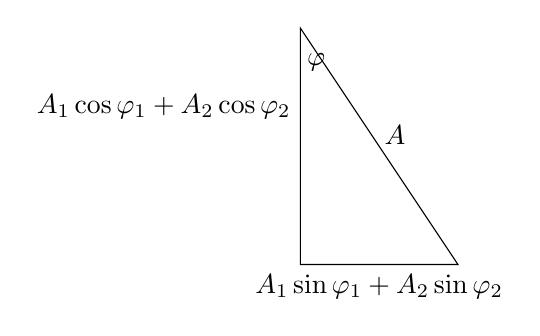
\begin{tikzpicture}
            \draw (0,0) -- (0,3) -- (2,0) -- cycle;
            \coordinate[label=left:$A_1 \cos \varphi_1+A_2 \cos \varphi_2$] (formulate1)
                at (0,2);
            \coordinate[label=below:$A_1 \sin \varphi_1+A_2 \sin \varphi_2$] (formulate2)
                at (1,0);
            \coordinate[label=below:$\varphi$] (phi) at (0.2,2.8);
            \coordinate[label=above:$A$] (A) at (1.2,1.4);
        \end{tikzpicture}
    \]

    \textbf{特殊情况}:

    \begin{enumerate}
        \item 若相位差$\varphi_2-\varphi_1=2 k \uppi \quad(k=0, \pm 1, \pm 2, \cdots)$,
            则\(A = A_1 + A_2\)
        \item 若相位差$\varphi_2-\varphi_1=2 (k+1) \uppi \quad(k=0, \pm 1, \pm 2, \cdots)$,
            则\(A = \left|A_1 - A_2\right|\)
    \end{enumerate}

    推广:多个同方向、同频率简谐运动合成仍为简谐运动。

\subsection{两个同方向不同频率的简谐振动的合成、拍}

\subsubsection{两个同方向不同频率的简谐振动的合成}

    两个振幅相同,初相位相同,在相同方向上以不同频率振动,
    振动表达式分别为:

    \[
        x_1\left(t\right) = A_1 cos\left(\omega_1 t + \varphi\right)
    \]

    \[
        x_2\left(t\right) = A_2 cos\left(\omega_2 t + \varphi\right)
    \]

    合成:

    \[
        x\left(t\right) = x_1\left(t\right) + x_2\left(t\right)
    \]

    \begin{equation}
        x=2 A \cos \left(\frac{\omega_2-\omega_1}{2} t\right) \cdot \cos \left(\frac{\omega_2+\omega_1}{2} t+\varphi\right)
    \end{equation}

    合振动不是简谐振动!

    $$
        x=A(t) \cos (\overline{\omega} t+\varphi)
    $$

    $A(t)=2 A \cos \left(\frac{\omega_2-\omega_1}{2} t\right)$
    随\(t \)缓变,
    $\cos (\overline{\omega} t+\varphi)=\cos \left(\frac{\omega_2+\omega_1}{2} t+\varphi\right)$
    随\(t \)快变:

    合振动可看作振幅缓变的简谐振动。

\subsubsection{拍}

    频率较大而频率之差很小的两个同方向简谐振动合成时,
    其合振动的振幅时而加强时而减弱的现象叫\textbf{拍}。

    \textbf{拍频}:单位时间内振动加强或减弱的次数叫拍频。

    拍频的值可由$\left|2 A \cos \left(\frac{\omega_2-\omega_1}{2}\right) t\right|=\left|2 A \cos \left(2 \uppi \frac{v_2-v_1}{2} t\right)\right|$
    取最大定出。

    相邻两最大满足

    $$
        2 \uppi \frac{v_2-v_1}{2} \cdot 0=0
    $$

    $$
        2 \uppi \frac{v_2-v_1}{2}T^{\prime}=\uppi
    $$

    拍频

    \begin{equation}
        v=\frac{1}{T^{\prime}}=\left|v_2-v_1\right|
    \end{equation}

    (\(T^{\prime}\)为振幅变化周期)

\subsection{两个相互垂直的同频率简谐振动的合成}

    分振动:

    \[
        x\left(t\right) = A_1 cos\left(\omega t + \varphi_1\right)
    \]

    \[
        y\left(t\right) = A_2 cos\left(\omega t + \varphi_2\right)
    \]

    合运动:

    \begin{equation}
        \frac{x^2}{A_1^2}+\frac{y^2}{A_2^2}-2 \frac{x}{A_1} \frac{y}{A_2} \cos \left(\varphi_2-\varphi_1\right)=\sin ^2\left(\varphi_2-\varphi_1\right)
    \end{equation}

    (椭圆)

\chapterimage{miku1.jpg} % Chapter heading image
\chapterspaceabove{6.25cm} % Whitespace from the top of the page to the chapter title on chapter pages
\chapterspacebelow{7.5cm} % Amount of vertical whitespace from the top margin to the start of the text on chapter pages

\chapter{机械波}

\section{机械波的产生和传播}

\subsection{机械波的基本概念}

    \textbf{波}是振动状态再空间的传播过程。

    \textbf{机械波}是机械振动在弹性介质中的传播过程。

    \textbf{电磁波}是交变电场在空间的传播过程。

    \textbf{弹性介质}(elastic medium):由无穷多个质元通过弹性力结合再一起形成的连续介质。

    \vspace{1em}
    要产生机械波,必须满足两个条件:

    \begin{enumerate}
        \item 要有波源(即振动源);
        \item 要有能够传播机械振动的弹性介质。
    \end{enumerate}

    \vspace{1em}
    机械波与电磁波的共同特征:

    \begin{enumerate}
        \item 具有一定的传播速度;
        \item 能够产生干涉、衍射现象;
        \item 伴随着能量的传播;
        \item 具有相似的数学表达式。
    \end{enumerate}

\begin{definition}[横波]
    质点的振动方向与波的传播方向垂直。
    横波中凸起的位置称为波峰,下凹的位置称为波谷。
\end{definition}

\begin{definition}[纵波]
    (又称为疏密波)质点的振动方向与波的传播方向平行。
\end{definition}

    在机械波中,横波只能在固体中出现;纵波可在气体、液体和固体中出现。
    空气中的声波是纵波。液体表面的波动情况较复杂,不是单纯的纵波或横波。

\textbf{波的几何描述}

    波阵面(波面, wave surface):相位相同的点连成的面;

    波线(波射线, wave ray):波的传播方向。

    \[
        \includegraphics[scale=0.4]{Chapter 07 images/pic1.jpg}
    \]

\subsection{描述机械波的物理量}

\begin{definition}[波速]
    单位时间内振动状态在介质中传播的距离称为波的传播速度,简称波速。
    在弹性介质中,机械波的传播速度取决于介质的惯性和弹性,
    也就是取决于介质的密度和弹性模量,与波源在介质中的运动速度无关。
\end{definition}

    在拉紧的弹性绳索中,横波的传播速度为

    \begin{align}
        u = \sqrt{\frac{F }{\lambda}}
    \end{align}

    式中\(F \)为绳中的张力,\(\lambda\)是绳的质量线密度。

    在固体中,既可以传播横波,也可以传播纵波,它们的传播速度分别为

    \begin{equation}
        u=\sqrt{\frac{G}{\rho}} \quad \text{(横波)}
    \end{equation}

    \begin{equation}
        u=\sqrt{\frac{E}{\rho}} \quad(\text{(纵波)})
    \end{equation}
    
    式中\(\rho\)是固体的密度,\(G\)和\(E\)分别是固体的切变模量(shear modulus)和杨氏模量
    (Young's modulus),它们是反应材料形变和內应力关系的物理量,其单位都是\(\mathrm{N \cdot m^{-2}}\)。

    在液体和液体中,纵波的传播速度为

    \begin{equation}
        u=\sqrt{\frac{K}{\rho}}
    \end{equation}

    式中\(K\)为介质的体积模量,\(\rho\)是气体或液体的密度。

    对于理想气体,根据分子动理论和热力学理论,可以证明理想气体中声波的传播速度为

    \begin{equation}
        u=\sqrt{\frac{\gamma p}{\rho}}=\sqrt{\frac{\gamma R T}{M}}
        \label{7-1-5}
    \end{equation}

    式中\(M\)是气体分子的摩尔质量,是气体的摩尔定压热容与摩尔定容热容之比,
    简称摩尔热容比,\(p\)是气体的压强,\(T\)是热力学温度,\(R \)是摩尔气体常量。
    式\ref{7-1-5}表明,气体中声波的传播速度不仅与气体的性质有关,还与温度有关。

    \begin{definition}[波长(wave length)]
    波的传播方向上相邻两振动状态完全相同的质点间的距离(一完整波的长度),用\(\lambda\)表示。
    \end{definition}

    \begin{definition}[周期]
    波传播一个波长的距离所用的时间,用\(T \)表示。
    \end{definition}

    波速\(u \)、波长\(\lambda\)和周期\(T \)三者之间有如下关系:

    \begin{equation}
        u=\frac{\lambda}{T}
        \label{7-1-6}
    \end{equation}

    \begin{definition}[频率]
        单位时间内波向前传播的完整波的数目,是周期的倒数,用\(\nu\)表示。
    \end{definition}

    于是式\ref{7-1-6}可改写为

    \begin{equation}
        u=\nu \lambda
    \end{equation}

    当波源和弹性介质没有相对运动(仅仅在介质中做振动)时,波源每做一次完全振动,
    波就会向前传播一个波长的距离,这表明波源的振动周期和振动频率在数值上与波的周期和波的频率是相等的,
    即两组物理量可以通用。如果波源与介质有相对运动,则两组物理量有差异,不可通用。

\section{平面简谐波的波动表达式}

\subsection{平面简谐波的波动表达式}

    波是运动状态的传播,介质的质点并不随波传播。

    设波源在\(t\)时刻的振动方程:

    $$
        y_O=A \cos (\omega t+\varphi)
    $$

    求波线\(x \)轴上平衡位置位于\(P \)点的质点的振动表达式。
    设\(P \)点与\(O \)点的距离为\(x \),因为波动从\(O \)传到\(P \)点处所需的时间为\(\dfrac{x }{u }\),
    所以\(P \)点处的质点在\(t\)时刻的位移与\(O \)点处的质点在\(t - \dfrac{x }{u }\)时刻的位移相同,即

    $$
        y_P(t)=y_O\left(t-\frac{x}{u}\right)=A \cos \left[\omega\left(t-\frac{x}{u}\right)+\varphi_0\right]
    $$

    质点的振动表达式(即位移随时间的变化规律),忽略下标\(P \),上式可写为

    \begin{equation}
        y(x, t)=A \cos \left[\omega\left(t-\frac{x}{u}\right)+\varphi_0\right]
        \label{7-2-1}
    \end{equation}

    这就是沿\(x\)轴正方向传播的平面简谐波的波动表达式,也称为波函数。
    
    当然,我们也可以用相位的超前与落后关系求出波函数。由于沿波的传播方向,
    波线上各点的振动相位依次落后,每隔一个波长的距离,后者比前者的相位落后\(2 \uppi \)。
    因此,如果已知波长\(\lambda\),则当波从\(O \)点传到\(P\)点时,\(P \)点的振动相位比\(O\)点
    落后\(\Delta \varphi = 2\uppi \dfrac{x}{\lambda}\),即

    \begin{equation}
        \varphi_P=\varphi_0-\Delta \varphi=\varphi_0-2 \uppi \frac{x}{\lambda}
    \end{equation}

    所以\(P \)点的振动表达式,即此波的波函数为

    \begin{equation}
        y(x, t)=A \cos \left(\omega t+\varphi_P\right)=A \cos \left(\omega t-\frac{2 \uppi}{\lambda} x+\varphi_0\right)
        \label{7-2-3}
    \end{equation}

    考虑到\(u = \dfrac{\lambda }{T }\),\(\omega = \dfrac{2 \uppi}{T } = 2 \uppi \nu\),
    \(\dfrac{\omega}{u}=\dfrac{2 \uppi}{\lambda}\),所以式\ref{7-2-1}和式\ref{7-2-3}两种形式的波动表达式实际上是等价的。
    同理可得波动表达式的其他形式,如

    \begin{equation}
        y(x, t)=A \cos \left[2 \uppi\left(\frac{t}{T}-\frac{x}{\lambda}\right)+\varphi_0\right]
    \end{equation}

    如果波动沿\(x \)轴的负方向传播,那么\(P \)点处质点的振动要比\(O \)点处的质点早开始\(\dfrac{x }{u }\)时间,
    即\(P\)点处的质点在\(t\)时刻的位移与\(O\)点处的质点在\(t + \dfrac{x }{u }\)的位移相同;
    从相位的角度来看,\(P \)点处质点的振动相位要比\(O \)点的相位超前$\Delta \varphi=2 \uppi \dfrac{x}{\lambda}=\dfrac{\omega}{u} x$,
    即

    $$
        \varphi_P=\varphi_O+\Delta \varphi=\varphi_O+2 \uppi \frac{x}{\lambda}
    $$

    所以\(P \)点处质点的振动表达式为

    \begin{equation}
        y(x, t)=A \cos \left[\omega\left(t+\frac{x}{u}\right)+\varphi_0\right]
    \end{equation}
    
    或

    \begin{equation}
        y(x, t)=A \cos \left(\omega t+\frac{2 \uppi}{\lambda} x+\varphi_0\right)
    \end{equation}

    \begin{equation}
        y(x, t)=A \cos \left[2 \uppi\left(\frac{t}{T}+\frac{x}{\lambda}\right)+\varphi_0\right]
    \end{equation}

\subsection{波动表达式的物理意义}

    当\(x \)一定时,如\(x = x_0\):

    \begin{equation}
        y(t)=A \cos \left[\omega\left(t-\frac{x_0}{u}\right)+\varphi_O\right]
    \end{equation}

    是\(x = x_0\)处质点的振动表达式。

    将波动表达式分别对时间求一阶和二阶偏导数,可得波线上任一质元\(P\)振动速度和加速度分别为

    \begin{equation}
        v(x, t)=\frac{\partial y(x, t)}{\partial t}=-A \omega \sin \left[\omega\left(t \pm \frac{x}{u}\right)+\varphi_0\right]
    \end{equation}
    
    \begin{equation}
        a(x, t)=\frac{\partial^2 y(x, t)}{\partial t^2}=-A \omega^2 \cos \left[\omega\left(t \pm \frac{x}{u}\right)+\varphi_0\right]
    \end{equation}
    
    \vspace{1em}

    当\(t \)一定时,如\(t = t_0\):

    \begin{equation}
        y(x)=A \cos \left[\omega\left(t_0-\frac{x}{u}\right)+\varphi_0\right]
    \end{equation}

    表示\(t_0\)时刻\(x\)轴上各质点的位移。

\section{平面简谐波的能量}

\subsection{波的能量}

    当波动在介质中传播时,各质元中的动能和势能总是同步变化的。在波峰、
    波谷处,动能势能同时为零;在平衡位置处,两者同时到达最大值。
    进一步的定量分析还表明,任一质元中的动能和势能不仅同步变化,
    而且大小总是相等的。这就是波动的能量特点。

    以固体棒中传播的纵波为例分析波动能量的传播:

    \[
        \includegraphics[scale=0.25]{Chapter 07 images/pic2.png}
    \]

    如图所示,假设匀质细棒的橫截面积为\(S \),棒的密度为\(\rho\),
    杨氏模量为\(E \),在棒中取一段长度为\(\rmd x\)的棒元,
    其体积为\(\rmd V=S\rmd x\),质量为\(\rmd m =\rho \rmd V=\rho S\rmd x\)。
    当波动传播到这里时,这段棒元由于振动而具有动能\(\rmd E_k\)。
    由于形变而具有弹性势能\(\rmd E_p\)。 不失一般性,设细棒中平面简谐波的波函数为

    \begin{equation}
        y(x, t)=A \cos \omega\left(t-\frac{x}{u}\right)
        \label{7-3-1}
    \end{equation}

    则该棒元振动速度为

    \begin{equation}
        v=\frac{\partial y}{\partial t}=-A \omega \sin \omega\left(t-\frac{x}{u}\right)
    \end{equation}

    所以该棒元的振动动能为

    \begin{equation}
        \mathrm{d} E_{\mathrm{k}}=\frac{1}{2} \mathrm{~d} m \cdot v^2=
        \frac{1}{2} \rho \mathrm{~d} V \cdot A^2 \omega^2 \sin ^2 \omega\left(t-\frac{x}{u}\right)
    \end{equation}

    设这段横截面积为\(S \)、长为\(\rmd x\)的棒元在拉力\(F \)的作用下,其长度的伸长量为\(\rmd y\),则

    \begin{equation}
        E=\frac{F / S}{\mathrm{~d} y / \mathrm{d} x}
    \end{equation}

    不难看出:$E$的物理意义就是其单位横伐面上的拉力$F / S$(称为应力),与单位长度上的伸长量$\rmd y / \mathrm{d} x$(称为应变)之比。
    将上式改写为
    
    \begin{equation}
        F=\frac{E S}{\mathrm{~d} x} \cdot \mathrm{~d} y
    \end{equation}

    将上式与胡克定律比较,的这段棒元的劲度系数为$k=\dfrac{E S}{\mathrm{~d} x}$,所以该棒元的弹性势能为

    \begin{equation}
        \mathrm{d} E_{\mathrm{p}}=\frac{1}{2} k(\mathrm{~d} y)^2=\frac{1}{2} \frac{E S}{\mathrm{~d} x}(\mathrm{~d} y)^2
        =\frac{1}{2} E \mathrm{~d} V\left(\frac{\partial y}{\partial x}\right)^2
        \label{7-3-6}
    \end{equation}

    又因为固体中纵波的传播速度为\(u = \sqrt{\dfrac{E }{\rho}}\),所以\(E = \rho u^2\),
    再由波动表达式\ref{7-3-1},可得应变为

    \begin{equation}
        \frac{\partial y}{\partial x}=-A \frac{\omega}{u} \sin \omega\left(t-\frac{x}{u}\right)
    \end{equation}

    将上式代入式\ref{7-3-6},整理后可得该棒元的弹性势能为

    \begin{equation}
        \mathrm{d} E_{\mathrm{p}}=\frac{1}{2} \rho A^2 \omega^2 \mathrm{~d} V \sin ^2 \omega\left(t-\frac{x}{u}\right)
    \end{equation}

    比较可得

    $$
        \mathrm{d} E_{\mathrm{k}}=\mathrm{d} E_{\mathrm{p}}=
        \frac{1}{2} \rho A^2 \omega^2 \mathrm{~d} V \sin ^2 \omega\left(t-\frac{x}{u}\right)
    $$

    即在波动传播到的任意位置,任意体积元\(\rmd V\)内的动能和势能总是相等的,且同步变化。
    所以体积元\(\rmd V\)中波动的总能量为

    \begin{equation}
        \mathrm{d} E=\mathrm{d} E_{\mathrm{k}}+\mathrm{d} E_{\mathrm{p}}=\rho A^2 \omega^2 \mathrm{~d} V \sin ^2 \omega\left(t-\frac{x}{u}\right)
        \label{7-3-9}
    \end{equation}

    \textbf{讨论}:

    \begin{enumerate}
        \item 每一体积元的动能和势能值相同,且同相位;
        \item 小体积元的机械能随时间作周期性变化。
    \end{enumerate}

\subsection{波的能量密度}

    人们将介质中单位体积内具有的波动能量称为波的能量密度(energy density of wave),记为$w$,由式\ref{7-3-9}可得

    \begin{equation}
        w=\frac{\mathrm{d} E}{\mathrm{~d} V}=\rho A^2 \omega^2 \sin ^2 \omega\left(t-\frac{x}{u}\right)
    \end{equation}

    上式说明,波的能量密度同样是时间\(t\)和空间坐标\(x\)的二元函数,且沿波的传播方向(\(x\)轴)以速度\(u\)传播。
    通常把能量密度在一个时间周期\(T\)内的平均值,称为平均能量密度,并用\(\overline{w}\)表示,即

    \begin{equation}
        \overline{w}=\frac{1}{T} \int_t^{t+T} w \mathrm{~d} t
    \end{equation}

    正弦函数:

    $$
        \begin{aligned}
            \overline{w} & =\frac{1}{T} \int_0^T w \mathrm{~d} t \\
            & =\frac{1}{T} \int_0^T \rho \omega^2 A^2 \sin ^2 \omega\left(t-\frac{x}{u}\right) \mathrm{d} t=\frac{1}{2} \rho \omega^2 A^2
        \end{aligned}
    $$

    即

    \begin{equation}
        \overline{w}=\frac{1}{2} \rho A^2 \omega^2
    \end{equation}

\subsection{能流、平均能流密度}

\begin{definition}[能流(面能量)]
    单位时间内通过某面积的能量——通过该面积的能流(energy flux, \(P\))。
\end{definition}

    对垂直于波的传播方向的面积\(S\)而言:

    \[
        \includegraphics[scale=0.25]{Chapter 07 images/pic3.png}
    \]

    能流

    \begin{equation}
        P=w u S=\rho A^2 \omega^2 u S \sin ^2 \omega\left(t-\frac{x}{u}\right)
    \end{equation}

    平均能流(average energy flux)

    \begin{equation}
        \overline{P}=\overline{w} u S
    \end{equation}

\subsubsection{波的能流密度}

\begin{definition}[能流密度]
    能流密度:与波传播方向垂直的单位面积上通过的能流。
\end{definition}

    \begin{definition}[平均能流密度(average energy flux density)]
    与波传播方向垂直的单位面积上通过的平均能流,也称为波的强度(波强,intensity of wave),用\(I \)表示,即

    \begin{equation}
        I=\frac{\overline{P}}{S}=\overline{w} u=\frac{1}{2} \rho u \omega^2 A^2
    \end{equation}
    \end{definition}

    由此可以证明,平面简谐波在无吸收的介质中传播时振动保持不变,
    球面波的波强与离开波源的距离的平方成反比。

\section{惠更斯原理、波的衍射、反射和折射}

\subsection{惠更斯原理}

    在波的传播过程中,所到达的每一点都可看作是发射子波的波源,
    在其后的任一时刻,这些子波的包络面就是新的波前。

    \[
        \includegraphics[scale=0.2]{Chapter 07 images/pic4.jpg}
    \]

\subsection{惠更斯原理的应用}

\subsubsection{波的衍射}

    波在传播过程中遇到障得物时,能够偏窝原来的直线传播方向,绕到障碍物后面的绕射现象,
    称为波的衍射(diffraction)。

    \begin{figure}[!htbp]
        \centering  % 居中放置
        \subfigure[缝宽\(a\)远大于波长\(\lambda\)]  % 为每个图片加上编号
        {
            \begin{minipage}[b]{.3\linewidth}
                \includegraphics[scale=0.2]{Chapter 07 images/pic5.png}
                % \caption{缝宽\(a \)远大于波长\(\lambda\)}
            \end{minipage}
        }
        \subfigure[缝宽\(a \)小于波长\(\lambda\)]
        {
            \begin{minipage}[b]{.3\linewidth}
                \includegraphics[scale=0.2]{Chapter 07 images/pic6.png}
                % \caption{缝宽\(a \)小于波长\(\lambda\)}
            \end{minipage}
        }
        % \caption{}
    \end{figure}
    
    \(\dfrac{a }{\lambda}\)越小,衍射越显著。

    波长较短的波衍射不显著,所以定向性较好。

    \begin{theorem}[折射定律]
    当波动从一种介质进入另一种介质时,由于在两种介质中的波速不同,
    在分界面上要发生折射现象。设在介质1中的波速是\(u_1\),在介质2中波速为\(u_2\),
    设\(MN \)为两种介质的分界面。

    \[
        \includegraphics[scale=0.25]{Chapter 07 images/pic7.jpg}
    \]

    \begin{equation}
        \frac{\sin i}{\sin r}=\frac{u_1}{u_2}=n_{21}
    \end{equation}

    式中\(n_{21}=\dfrac{u_1}{u_2}\)称为介质2对介质1的相对折射率。
\end{theorem}

\section{波的干涉}

\subsection{波的叠加原理}

    几列波相遇之后, 仍然保持它们各自原有的特征(频率、波长、振幅、振动方向等)不变,
    相遇之后并按照原来的方向继续前进,好象没有遇到过其他波一样。

    在相遇区域内任一点的振动,为各列波单独存在时在该点所引起的振动位移的矢量和。
    
\subsection{波的干涉}

    频率相同、振动方向平行、相位相同或相位差恒定的两列波相遇时,
    使某些地方振动始终加强,而使另一些地方振动始终减弱的现象,
    称为波的干涉(interference)现象。

    两相干波源振动规律:

    \[
        \includegraphics[scale=0.3]{Chapter 07 images/pic8.png}
    \]

    $$
        y_1=A_1 \cos \left(\omega t-\frac{2 \uppi r_1}{\lambda}+\varphi_1\right)
    $$

    $$
        y_2=A_2 \cos \left(\omega t-\frac{2 \uppi r_2}{\lambda}+\varphi_2\right)
    $$

    \(P \)点的合振动为

    \begin{equation}
        y=y_1+y_2=A \cos (\omega t+\varphi)
    \end{equation}

    其中

    \begin{equation}
        \tan \varphi=\dfrac{A_1 \sin \left(\varphi_1-\dfrac{2 \uppi r_1}{\lambda}\right)+
        A_2 \sin \left(\varphi_2-\dfrac{2 \uppi r_2}{\lambda}\right)}{A_1 \cos \left(\varphi_1-\dfrac{2 \uppi r_1}{\lambda}\right)+A_2 \cos \left(\varphi_2-\dfrac{2 \uppi r_2}{\lambda}\right)}
    \end{equation}

    \begin{equation}
        A=\sqrt{A_1^2+A_2^2+2 A_1 A_2 \cos \left(\varphi_2-\varphi_1-2 \uppi \frac{r_2-r_1}{\lambda}\right)}
    \end{equation}

    两个波源振动传播到\(P\)点的引起的两个振动相位差值

    \begin{equation}
        \Delta \varphi=\varphi_2-\varphi_1-2 \uppi \frac{r_2-r_1}{\lambda}
    \end{equation}

    干涉叠加加强或减弱取决于\(\Delta \varphi\)。凡是满足

    \begin{equation}
        \Delta \varphi=\varphi_2-\varphi_1-2 \uppi \frac{r_2-r_1}{\lambda}= \pm 2 k \uppi, \quad k=0,1,2, \cdots
    \end{equation}

    的空间各点,\(A = A_{max} = A_1+A_2\),这些点的合振幅最大,称为\textbf{干涉加强},或\textbf{相长干涉}。

    凡是满足

    \begin{equation}
        \Delta \varphi=\varphi_2-\varphi_1-2 \uppi \frac{r_2-r_1}{\lambda}= \pm(2 k-1) \uppi, \quad k=1,2,3, \cdots
    \end{equation}

    的空间各点,\(A = A_{min} = \left|A_1-A_2\right|\),这些点的合振幅最小,称为\textbf{干涉减弱}。
    如果\(A_1=A_2\),则\(A = A_{min} = 0\),即该点的合振幅为零,这称为\textbf{相消干涉}。

    \(P\)波强度

    \begin{equation}
        I=I_1+I_2+2 \sqrt{I_1 I_2} \cos \Delta \varphi
        \label{7-5-7}
    \end{equation}

    \begin{enumerate}
        \item 相干波源在\(P\)点波强\(\neq I_1+I_2\), 而是多出一与位置有关的干涉项;
        \item 对确定点\( P\),\(\Delta \varphi\)为固定值,波强为确定值,不随时间变化;
        \item 对不同点,\(\Delta \varphi\)不同,\(I\)也不同,有强弱分布,产生干涉现象;
        \item 当\(\Delta \varphi\)为\(\uppi\)的偶数倍时,波强达极大值(干涉极大);当\(\Delta \varphi\)为\(\uppi\)的奇数倍时,干涉极小。
    \end{enumerate}

    当\(I_1=I_2=I_0\),则式\ref{7-5-7}可以写成

    \begin{equation}
        I=2 I_0(1+\cos \Delta \varphi)=4 I_0 \cos ^2 \frac{\Delta \varphi}{2}
    \end{equation}

\section{驻波}

\subsection{驻波的形成和特点}

    两列\textbf{振幅相同}的\textbf{相干波}在同一直线上\textbf{沿相反方向传播}时由于相干叠加所产生的波称为\textbf{驻波}。

    波的干涉是特定条件下的波叠加, 驻波又是特定条件下的波的干涉。

    \[
        \includegraphics[width=\linewidth]{Chapter 07 images/pic9.png}
    \]

\subsection{驻波方程}

    设有两列波相向传播,沿\(x\)轴正向传播的波为

    $$
        y_1(x, t)=A \cos \left(\omega t-\frac{2 \uppi x}{\lambda}+\varphi_1\right)
    $$

    沿\(x\)轴负向传播的波为

    $$
        y_2(x, t)=A \cos \left(\omega t+\frac{2 \uppi x}{\lambda}+\varphi_2\right)
    $$

    则合成波(即驻波)的表达式为:

    \begin{equation}
        y_{\text{合}}(x, t)=y_1(x, t)+y_2(x, t)=
        2 A \cos \left(\frac{2 \uppi}{\lambda} x+\frac{\varphi_2-\varphi_1}{2}\right) \cos \left(\omega t+\frac{\varphi_2+\varphi_1}{2}\right)
        \label{7-6-1}
    \end{equation}

    式\ref{7-6-1}即为驻波方程。

\subsubsection{波腹和波节}

    \begin{equation}
        A_{\text{合}}=\left|2 A \cos \left(\frac{2 \uppi}{\lambda} x+\frac{\varphi_2-\varphi_1}{2}\right)\right|
    \end{equation}

    驻波上各点的振幅不同,其大小与位置\(x \)有关。
    当\({\displaystyle \left|2 A \cos \left(\frac{2 \uppi}{\lambda} x+\frac{\varphi_2-\varphi_1}{2}\right)\right|=1}\),
    合振幅达到最大值(\(A_{\text{合}} = A_1+A_2\)),这就是波腹。波腹的位置条件为

    \begin{equation}
        \frac{2 \uppi}{\lambda} x+\frac{\varphi_2-\varphi_1}{2}= \pm k \uppi, \quad k=0,1,2, \cdots
    \end{equation}

    当\({\displaystyle 2 A \cos \left(\frac{2 \uppi}{\lambda} x+\frac{\varphi_2-\varphi_1}{2}\right)=0}\),
    合振幅为零(\(A_{\text{合}} = 0\)),这就是波节。波节的位置条件为

    \begin{equation}
        \frac{2 \uppi}{\lambda} x+\frac{\varphi_2-\varphi_1}{2}= \pm(2 k+1) \frac{\uppi}{2}, \quad k=0,1,2, \cdots
    \end{equation}

    所以相邻两波节或波腹之间的距离为

    \begin{equation}
        \Delta x=x_{k+1}-x_k=\frac{\lambda}{2}
    \end{equation}

\subsubsection{振动相位}

    驻波方程\ref{7-6-1}中没有\(x\)坐标,表示没有相位的传播。

    相邻两波节之间的各质点的振动相位相同;波节两侧的各质点的振动相位相反。

    驻波(已经是叠加波)不是振动相位的传播过程,驻波的波形不发生定向传播。

\subsubsection{驻波的能量}

    驻波的能量在相邻的波腹和波节间往复变化,在相邻的波节间发生动能和势能间的转换,
    动能主要集中在波腹,势能主要集中在波节,但无长距离的能量传播。

\subsection{半波损失}

    入射波从波疏介质到波密介质,在两者的界面上,反射波在反射点出现半波损失,
    引起\(\uppi\)相位的突变。

    由入射波与反射波产生驻波 与 “半波损失”。

    \[
        \includegraphics[width=\linewidth]{Chapter 07 images/pic10.png}
    \]

\part{大学物理B(下)}

\chapterimage{miku2.jpg} % Chapter heading image
\chapterspaceabove{6.25cm} % Whitespace from the top of the page to the chapter title on chapter pages
\chapterspacebelow{7.5cm} % Amount of vertical whitespace from the top margin to the start of the text on chapter pages

\chapter{真空中的恒定磁场}

\section{恒定电流}

\subsection{电流 \quad 电流密度}

\begin{equation}
    \overrightarrow{j} = \deriv{I}{S_0} \overrightarrow{e}_{\text{n}}
\end{equation}

\begin{itemize}
    \item 方向:改点正电荷运动的方向,即$\overrightarrow{e}_{\text{n}}$;
    \item 大小:$j = \dderiv{I}{S_0} = \dderiv{I}{S \cos \theta}$。
\end{itemize}

通过面积元的电流为

\begin{equation}
    I = \int_S \overrightarrow{j} \cdot \rmd \overrightarrow{S}
\end{equation}

\subsection{电流的连续性方程 \quad 电路恒定的条件}

在导体内任取一封闭曲面$S$,由电荷守恒

\begin{equation}
    \oint_S \overrightarrow{j} \cdot \rmd \overrightarrow{S} = - \deriv{Q}{t}
\end{equation}

由$Q = \int_V \rho \rmd V$ ($\rho = \rho(x,y,z,t)$为电荷体密度分布函数),

\begin{equation}
    \oint_S \overrightarrow{j} \cdot \rmd \overrightarrow{S} = \int_V \pderiv{\rho}{t} \rmd V
\end{equation}

\subsection{欧姆定律及其微分形式}

由电阻定律,

\begin{equation}
    R = \rho \frac{l}{S}
\end{equation}

电流在不均匀的导体中流动:

\begin{equation}
    R = \int \rmd R = \int \rho \frac{\rmd l}{S}
\end{equation}

沿电场线方向,取长$\rmd l$、横截面积$\rmd S$的微流管,电阻率为$\rho$,则

\begin{equation}
    j = \frac{1}{\rho}\left(-\deriv{V}{l}\right) = \sigma E
\end{equation}

矢量形式为

\begin{equation}
    \overrightarrow{j} = \sigma \overrightarrow{E}
\end{equation}

\begin{exercise}
如图所示,高度为\(h\)的两个共轴金属圆环,其内环的外半径和外环的内半径分别为\(R_1\)和\(R_2\)。两环间充满电阻率为\(\rho\)的均匀导电材料($\rho$4远大于金属圆环的电阻率)。
当圆环之间加上电压\(U\)后,电流沿径向由内向外流动。试求

\begin{enumerate}
    \item 两环之间导电材料的总电阻;
    \item 两环之间距离为\(r\)处电流密度的大小和方向。
\end{enumerate}

\centering{\includegraphics{graphics/p12.1.pdf}}
\end{exercise}

在导电材料上任取一半径为$r$,宽度为$\rmd r$,高度为$h$的薄圆环,其侧面积为$2 \uppi r h$,则薄圆环的径向电阻为

\begin{equation*}
    \rmd R = \rho \frac{\rmd r}{2 \uppi rh}
\end{equation*}

所以整个导电材料的径向总电阻为

\begin{equation*}
    R = \int \rmd R = \int_{R_1}^{R_2} \rho \frac{\rmd r}{2 \uppi rh} \ln \frac{R_2}{R_1}
\end{equation*}

由欧姆定律可得导电材料中的径向总电流为

\begin{equation*}
    I = \frac{U}{R} = \frac{2 \uppi h U}{\rho \ln(R_2/R_1)}
\end{equation*}

于是在距离环心为\(r\)处电流密度的大小为

\begin{equation*}
    j = \frac{I}{S} = \frac{I}{2 \uppi r h} = \frac{U}{r \rho \ln(R_2/R_1)}
\end{equation*}

\subsection{电源\quad 电动势}

电动势

\begin{equation}
    \mathscr{E} = \int_{-}^{+} \overrightarrow{E}_{\text{k}} \cdot \rmd l
\end{equation}

闭合回路的总电动势

\begin{equation}
    \mathscr{E} = \oint_L \overrightarrow{E}_{\text{k}} \cdot \rmd l
\end{equation}

\section{磁场 \quad 磁感应强度}

定义磁感应强度\(\overrightarrow{B}\)的大小为

\begin{equation}
    B = \frac{F_{\text{max}}}{qv}
\end{equation}

运动电荷在磁场中受到的磁场力可表示为

\begin{equation}
    \overrightarrow{F} = q \overrightarrow{v} \times \overrightarrow{B}
\end{equation}

这就是运动电荷在磁场中受到的磁场力,通常称为\textbf{洛伦兹力}。

\section{毕奥-萨伐尔定律}

\subsection{毕奥-萨伐尔定律}

\begin{theorem}[毕奥-萨伐尔定律]
电流元\(I \rmd \overrightarrow{l}\)在空间某点\(P\)处激发的磁感应强度\(\rmd \overrightarrow{B}\)的大小与电流元\(I\rmd \overrightarrow{l}\)的大小成正比,与电流元\(I\rmd \overrightarrow{l}\)到场点\(P\)的距离\(r\)的平方成反比,与电流元\(I\rmd \overrightarrow{l}\)和径矢\(\overrightarrow{r}\)之间的夹角\(\theta\)的正弦成正比,即

\begin{equation}
    \rmd B = \frac{\mu_0}{4 \uppi} \cdot \frac{I \rmd l \sin \theta}{r^2}
    \label{13}
\end{equation}

\(\rmd \overrightarrow{B}\)的方向与\(I \rmd \overrightarrow{l} \times \overrightarrow{r}\)的方向相同,即\(\rmd \overrightarrow{B}\)的方向与\(I \rmd \overrightarrow{l}\)和\(\overrightarrow{r}\)的方向符合右手螺旋定律。将式\ref{13}写成矢量形式,则有

\begin{equation}
    \rmd \overrightarrow{B} = \frac{\mu_0}{4 \uppi} \frac{I \rmd \overrightarrow{l} \times \overrightarrow{e_r}}{r^2} = \frac{\mu_0}{4 \uppi} \frac{I \rmd \overrightarrow{l} \times \overrightarrow{r}}{r^3}
\end{equation}

其中\(\overrightarrow{e_r} = \dfrac{\overrightarrow{r}}{r}\)为\(\overrightarrow{r}\)方向的单位矢量。此即毕奥-萨伐尔定律的数学表达式。

根据场强叠加原理

\begin{equation}
    \overrightarrow{B} =\int_{L} = \frac{\mu_0}{4 \uppi} \int_L \frac{I \rmd \overrightarrow{l} \times \overrightarrow{e_r}}{r^2}
\end{equation}
\end{theorem}

\subsection{毕奥-萨伐尔定律的应用}

\subsubsection{载流直导线的磁场}

(教材Page. 11)

真空中有一根长度为\(l\)、通有恒定电流\(I\)的直导线\(A_1A_2\),试求载流直导线附近任意一点\(P\)处的磁感应强度\(B\)。已知\(P\)点到直导线的垂直距离为\(a\)。

\begin{equation}
    B = \frac{\mu_0 I}{2 \uppi a}
\end{equation}

“无限长”载流直导线产生的磁场分布具有轴对称性和轴向平移不变性。

\subsubsection{圆电流轴线上任意一点的磁场}

(教材Page. 12)

真空中有一载流圆环,通有恒定电流\(I\),已知圆环的半径为\(R\),试求圆环轴线上任意一点\(P\)处的磁场强度。

\begin{equation}
    B = \frac{\mu_0 I R^2}{2 \left(R^2 + x^2\right)^{3/2}} = \frac{\mu_0 I}{2R} \cdot \sin^3 \theta = B_0 \cdot \sin^3 \theta
\end{equation}
其中\(B_0\)为圆电流在圆心处激发的磁场。

如果有一个平面载流线圈,线圈中的电流为\(I\),线圈的面积为\(S\),线圈的总匝数为\(N\),则该平面载流线圈的磁矩定义为
\begin{equation}
    \overrightarrow{m} = NIS \overrightarrow{e}_n
\end{equation}
式中,\(\overrightarrow{e}_n\)为线圈平面法向的单位矢量,它与线圈中的电流方向符合右手螺旋法则。于是圆电流轴线上任意一点的磁感应强度公式还可以写为
\begin{equation}
    B = \frac{\mu_0 I R^2}{2 \left(R^2 + x^2\right)^{3/2}} = \frac{\mu_0 m}{2 \uppi \left(R^2 + x^2\right)^{3/2}}
\end{equation}

\subsubsection{载流密绕直螺线管线圈在其轴线上的磁场}

(教材Page. 14)

设真空中有一半径为\(R\)的均匀密绕的载流直螺线管线圈,其电流为\(I\)。管长为\(l\),沿轴线单位长度的匝数为\(n\)。试求螺线管内轴线上任意一\(P\)处的磁感应强度\(\overrightarrow{B}\)。

当管长\(l >> R\)时,螺线管可近似为无限长,则
\begin{equation}
    B = \mu_0 n I
\end{equation}
在螺线管线圈的端口处
\begin{equation}
    B = \frac{1}{2} \mu_0 n I
\end{equation}

\subsubsection{运动电荷的磁场}

(教材Page. 16)

设导体中单位体积内有\(n\)个做定向运动的电荷,每个电荷的电荷量为\(q\)(不妨假设\(q > 0\)),以平均漂移速度\(\overrightarrow{v}\)沿电流元\(I \rmd \overrightarrow{l}\)方向匀速运动而形成电流\(I\),如果电流元的横截面积为\(S\),则单位时间通过横截面积\(S\)的电荷量为\(nqSv\),亦即\(I = nqSv\)。于是每一个以速度\(v\)运动的电荷在场点\(P\)处产生的磁感应强度\(\overrightarrow{B}\)就是
\begin{equation}
    \overrightarrow{B} = \deriv{\overrightarrow{B}}{N} = \frac{\mu_0}{4 \uppi} \cdot \frac{q \overrightarrow{v} \times \overrightarrow{r}}{r^3}
\end{equation}

\section{真空中恒定磁场的基本定理}

\subsection{磁感应线}

磁感应线上任一点的切线方向就是该点处磁感应强度\(\overrightarrow{B}\)的方向,而空间任一点处磁感应线的疏密程度则反映了该处磁场的强弱。

\subsection{磁通量}

在磁场中某点处,通过与磁场方向垂直的单位面积上的磁感应线的根数就等于该点处磁感应强度的大小
\begin{equation}
    B = \deriv{N}{S_{\perp}}
\end{equation}

将磁场中通过某个曲面的磁感应线的根数,称为该曲面的磁通量
\begin{equation}
    \Phi = BS \cos \theta = \overrightarrow{B} \rmd \overrightarrow{S}
\end{equation}
非均匀磁场中任意曲面\(S\)
\begin{equation}
    \Phi = \int \rmd \Phi = \int_S B \cos \theta \rmd S = \int_S \overrightarrow{B} \rmd \overrightarrow{S}
\end{equation}

\subsection{磁场的高斯定理}

\begin{theorem}[磁场的高斯定理]
磁感应强度对任意一个闭合曲面的磁通量必等于零,即
\begin{equation}
    \oint_S \overrightarrow{B} \cdot \rmd \overrightarrow{S} = 0
\end{equation}
\end{theorem}


\emph{注意}:与静电场的高斯定理$\oint \overrightarrow{E} \rmd \overrightarrow{S} = \dfrac{1}{\varepsilon_0} \sum q$有本质区别。静电场是有源场,磁场是无源场。

\subsection{真空中磁场的安培环路定理}

\begin{theorem}[真空中磁场的安培环路定理]
在真空中磁感应强度 $\overrightarrow{B}$对任意一个闭合环路$L$的环流(即线积分)等于真空中的磁导率$\mu_ O $与该闭合四路 $L $所包围的电流的代数和 $\sum I_ i$之积
\begin{equation}
    \oint_L \overrightarrow{B} \cdot \rmd \overrightarrow{l} = \mu_0 \sum I_i
\end{equation}
\end{theorem}

对电流连续分布的载流体情形,安培环路定理可表示为
\begin{equation}
    \oint_L \overrightarrow{B} \cdot \rmd \overrightarrow{l} = \mu_0 \int_S \overrightarrow{j} \cdot \rmd \overrightarrow{S}
\end{equation}

\subsection{安培环路定理的应用}

一根半径为\(R\)的“无限长”的载流直圆柱形导体,电流沿轴向流动,且在圆柱体的横截面上均匀分布。试求圆柱体内外磁感应强度的分布。

(教材Page. 21)

\begin{equation*}
    \begin{aligned}
        & B = \frac{\mu_0 I}{2 \uppi r} (r \geq R) \\
        & B = \frac{\mu_0 I}{2 \uppi R^2} r (0 < r < R)
    \end{aligned}
\end{equation*}

\(\overrightarrow{B}\)的方向沿圆周的切线方向,并与圆柱体上的电流\(I\)成右手螺旋关系。

\section{磁场对电流的作用}

\subsection{安培定律}

\begin{theorem}[安培定律]
\begin{equation}
    \rmd F = B I \rmd l \sin \theta
\end{equation}
\end{theorem}

矢量表达式
\begin{equation}
    \rmd \overrightarrow{F} = I \rmd \overrightarrow{l} \times \overrightarrow{B}
\end{equation}

对任意形状的载流导线在磁场中受到的安培力
\begin{equation}
    \overrightarrow{F} = \int_L \rmd \overrightarrow{F} = \int_L I \rmd \overrightarrow{l} \times \overrightarrow{B}
\end{equation}

在匀强磁场中任意形状的一段载流导体所受的安培力,等效于该导线的起点和终点之间的一根载流直导线在同一磁场中所受安培力。

\subsection{无限长平行载流直导线间的相互作用}

假设真空中有两根相立平行的“无限长”载流直导线,相距为$d$,两导线受力均为
\begin{equation}
    F = \frac{\mu_0 I_1 I_2}{2 \uppi d}
\end{equation}
当两载流直导线通有同向电流时相互吸引,通有反向电流则相互排斥。

\subsection{均匀磁场对载流线圈的作用}

磁场对线圈有一个磁力矩的作用,其大小为
\begin{equation*}
    M = NISB \cos \varphi
\end{equation*}
式中\(S = l_1l_2\)为线圈面积。若线圈共有N匝,则
\begin{equation}
    M = NISB \cos \varphi
\end{equation}

令\(\overrightarrow{e}_n\)与\(\overrightarrow{B}\)夹角为\(\theta\),则
\begin{equation}
    M = NISB \sin \theta = m B \sin \theta
\end{equation}
式中\(m = NIS\)是线圈磁矩的大小。磁力矩\(\overrightarrow{M}\)的方向与矢量积\(\overrightarrow{e}_n \times \overrightarrow{B}\)的方向相同。由于磁矩也是矢量,其方向就是线圈平面的发现方向,即
\begin{equation}
    \overrightarrow{m} = NIS \overrightarrow{e}_n
\end{equation}
所以线圈在均匀磁场中受到的磁力矩的矢量表达式为
\begin{equation}
    \overrightarrow{M} = \overrightarrow{m} \times \overrightarrow{B}
\end{equation}

\subsection{磁场力和磁力矩的功}

若回路中的电流\(I\)恒定不变,当导线从\(ab\)位置运动到\(a\prime b \prime\)位置时,磁场力做的总功为
\begin{equation}
    A = \int \rmd A = \int_{x_1}^{x_2} IBL \rmd x = IBL (x_2 - x_1) = I \cdot \Delta \varphi
\end{equation}

当载流线圈在磁力矩的作用下,其法线方向与磁场的夹角由\(\theta_1\)转到\(\theta_2\)时,同时保持线圈中的电流\(I\)恒定不变,则磁力矩所做的功为
\begin{equation}
    \begin{aligned}
        A = \int \rmd A & = \int_{\theta_1}^{\theta_2} I \cdot \rmd (SB \cos \theta) \\
        & = I (SB \cos \theta_2 - SB \cos \theta_2) = I \cdot (\Phi_1 - \Phi_2) = I \cdot \Delta \Phi
    \end{aligned}
\end{equation}

当电流\(I\)恒定不变时,做功可表示为
\begin{equation}
    \rmd A = I \cdot \rmd \Phi \quad \text{或} \quad A = \int \rmd A = I \cdot \Delta \Phi
\end{equation}

如果线圈总匝数为\(N\),则磁力矩所做的功为
\begin{equation}
    \rmd A = NI \cdot \rmd \Phi \quad \text{或} \quad A = \int \rmd A = NI \cdot \Delta \Phi
\end{equation}

\chapterimage{miku3.png} % Chapter heading image
\chapterspaceabove{6.25cm} % Whitespace from the top of the page to the chapter title on chapter pages
\chapterspacebelow{7.5cm} % Amount of vertical whitespace from the top margin to the start of the text on 

\chapter{磁介质}

\section{磁介质的磁化}

\subsection{磁介质的磁化 \quad 相对磁导率}

被磁化后的磁介质会激发附加磁场\(\overrightarrow{B^\prime}\),从而影响介质内外的磁场分布。磁介质内的磁感应强度为
\begin{equation}
    \overrightarrow{B} = \overrightarrow{B_0} + \overrightarrow{B^ \prime}
\end{equation}

相对磁导率
\begin{equation}
    \mu_r = \frac{B}{B_0}
\end{equation}

相对磁导率\(\mu_r\)的大小只与磁介质的性质有关,根据\(\mu_r\)的大小将磁介质分成顺磁质、抗磁质和铁磁质三类。

\begin{enumerate}
    \item 顺磁质\(\mu_r\)略大于1,即\(\mu_r \approx 1 + 10^{-4} > 1\)
    \item 抗磁质\(\mu_r\)略大于1,即\(\mu_r \approx 1 - 10^{-5} < 1\)
    \item 铁磁质\(\mu_r >> 1\),磁化后产生的磁场\(\overrightarrow{B^\prime}\)的方向与原磁场\(\overrightarrow{B_0}\)的方向相同,且\(\overrightarrow{B^\prime} >> \overrightarrow{B_0}\)
\end{enumerate}

\subsection{磁化强度和磁化电流}

\begin{definition}[磁化强度]
    将磁介质中单位体积内分子磁矩的矢量和称为\emph{磁化强度},并用\(\overrightarrow{M}\)来表示,即
    \begin{equation}
        \overrightarrow{M} = \frac{\sum \overrightarrow{m_{\text{分子}}}}{\Delta V} = \frac{\sum \overrightarrow{m} + \sum \Delta \overrightarrow{m}}{\Delta V}
    \end{equation}
    在国际单位制中,\(\overrightarrow{M}\)的单位为\(\mathrm{A} \cdot \mathrm{m}^{-1}\)。
\end{definition}

设有一“无限长”的载流直螺线管,管内充满均匀磁介质,电流在螺线管内激发匀强磁场。在此磁场中磁介质被均匀磁化,这时磁介质中各个分子电流平面将转到与磁场的方向相垂直。对磁介质的整体来说,未被抵消的分子电流是沿着柱面流动的,称为安培表面电流(或叫磁化面电流),用\(I_s\)表示。沿轴线单位长度上的磁化电流称为磁化电流密度,用\(\overrightarrow{j_s}\)表示。于是,沿棒的轴线方向长为\(L\)的表面上,磁化电流的大小为\(I_s = j_s L\)。介质被磁化的程度越大,介质表面的磁化电流越大。

\begin{figure}[!h]
    \centering
    \includegraphics[width = .4\textwidth]{graphics/磁化电流.png}
\end{figure}

对顺磁性物质,安培表面电流和螺线管上导线中的电流方向相同;对抗磁性物质,则两者方向相反。

即当磁化强度的方向与介质表面平行时,磁介质表面磁化电流密度的大小等于该处磁化强度的大小,即
\begin{equation}
    M = \frac{\sum  \overrightarrow{m}_{\text{分子}}}{\Delta V} = \frac{j_s L S}{L S} = j_s
\end{equation}

如果磁化强度的方向与介质表面不平行,可以证明
\begin{equation}
    \overrightarrow{j}_s = \overrightarrow{M} \times \overrightarrow{e}_n
\end{equation}
式中\(\overrightarrow{e}_n\)为磁介质表面的外法线单位矢量。该式表明,磁化强度\(\overrightarrow{M}\)沿磁介质表面的切向分量等于介质表面的磁化电流密度。

可以证明:磁化强度\(\overrightarrow{M}\)与磁化电流\(I_s\)之间的普遍关系为
\begin{equation}
    \oint_L \overrightarrow{M} \cdot \rmd \overrightarrow{L} = \sum I_s
    \label{13-6}
\end{equation}

\section{有磁介质存在时的安培环路定理和高斯定理}

\subsection{有磁介质存在时的安培环路定理 \quad 磁场强度}

\begin{theorem}[有磁介质存在时的安培环路定理]
有磁介质存在时,空间任意一点的磁感应强度\(\overrightarrow{B}\)应由导线中的传导电流\(I_0\)和磁介质表面的磁环电流\(I_s\)共同产生,因此有磁介质存在时,磁场的安培环路定理应写成
\begin{equation}
    \oint_L \overrightarrow{B} \cdot \rmd \overrightarrow{L} = \mu_0 \left(\sum I_0 + \sum I_s\right)
\end{equation}
式中,\(\sum I_0\)是穿过闭合回路\(L\)所围面积的传导电流的代数和,\(\sum I_s\)时磁化电流的代数和。
\end{theorem}

如果将磁化强度\(\overrightarrow{M}\)与磁化电流\(I_s\)的普遍关系式\ref{13-6}代入上式,则有
\begin{equation}
    \oint_L \overrightarrow{B} \cdot \rmd \overrightarrow{L} = \mu_0 \left(\sum I_0 + \oint_L \overrightarrow{M} \cdot \rmd \overrightarrow{L}\right)
\end{equation}
或写为
\begin{equation}
    \oint_L \left(\frac{\overrightarrow{B}}{\mu_0} - \overrightarrow{M}\right) \cdot \rmd \overrightarrow{L} = \sum I_0
    \label{13-9}
\end{equation}

\begin{definition}[磁化强度]
    引入一个新的辅助物理量,称为\emph{磁场强度},用\(\overrightarrow{H}\)表示,并定义
    \begin{equation}
        \overrightarrow{H} = \frac{\overrightarrow{B}}{\mu_0} - \overrightarrow{M}
    \end{equation}
\end{definition}
\begin{theorem}[有磁介质时的安培环路定理]
    则式\ref{13-9}可写为
    \begin{equation}
        \oint_L \overrightarrow{H} \cdot \rmd \overrightarrow{L} = \sum I_0
        \label{13-11}
    \end{equation}
\end{theorem}

式\ref{13-11}称为有磁介质时的安培环路定理,它表明磁场强度\(\overrightarrow{H}\)沿任一闭合回路\(L\)的线积分(或环流)等于通过该回路\(L\)所围成面积的传导电流的代数和。

\subsection{磁介质的磁化特性}

在各向同性的磁介质内部,任意一点的磁化强度\(\overrightarrow{M}\)和磁场强度\(\overrightarrow{H}\)成正比,即
\begin{equation}
    \overrightarrow{M} = \chi_m \overrightarrow{H}
\end{equation}
式中\(\chi_m\)为比例系数,称为介质的\emph{磁化率},对于顺磁质,\(\chi_m > 0\),表明顺磁质中\(\overrightarrow{M}\)和\(\overrightarrow{H}\)的方向相同;对于抗磁质,\(\chi_m > 0\),表明抗磁质中\(\overrightarrow{M}\)和\(\overrightarrow{H}\)的方向相反。

于是
\begin{equation}
    \overrightarrow{B} = \mu_0 (1 + \chi_m)\overrightarrow{H} = \mu_0 \mu_r \overrightarrow{H}= \mu \overrightarrow{H}
\end{equation}
式中
\begin{equation}
    \mu_r = 1 + \chi_m, \quad \mu = \mu_0\mu_r
\end{equation}
\(\mu_r\)和\(\mu_0\)分别称为磁介质的相对磁导率和绝对磁导率(有时也简称为磁导率)。

对于真空中的磁场,由于\(\overrightarrow{M} = 0\),则\(\chi_m = 0\),\(\overrightarrow{B} = \mu_0 \overrightarrow{H}\),这表明真空的相对磁导率\(\mu_r = 1\)。

\subsection{有磁介质存在时的高斯定理}

\begin{theorem}[有磁介质存在时的高斯定理]
    \begin{equation}
        \oint_S \overrightarrow{B} \cdot \rmd \overrightarrow{S} = 0
    \end{equation}
\end{theorem}

\chapterimage{miku1.jpg} % Chapter heading image
\chapterspaceabove{6.25cm} % Whitespace from the top of the page to the chapter title on chapter pages
\chapterspacebelow{7.5cm} % Amount of vertical whitespace from the top margin to the start of the text on chapter pages

\chapter{电磁感应}

\section{电磁感应的基本定律}

\subsection{电磁感应现象}

当通过导体回路的磁通量随时间发生变化时,回路中就有感应电动势产生,从而产生感应电流。这个磁通量的变化可以是由磁场变化引起的,也可以是由于导体在磁场中运动或导体回路中的一部分切割磁力线的运动而产生的。

\subsection{楞次定律}

1833年,楞次(Lenz)在进一步概括了大量实验结果的基础上,得出了确定感应电流方向的法则,称为楞次定律。这就是:闭合回路中产生的感应电流具有确定的方向,它总是使感应电流所产生的通过回路面积的磁通量,去补偿或者反抗引起感应电流的磁通量的变化。

    \begin{figure}[!htbp]
        \centering  % 居中放置
        \subfigure[磁棒插入导体圆环时]  % 为每个图片加上编号
        {
            \begin{minipage}[b]{.3\linewidth}
                \includegraphics[width=0.9\linewidth]{graphics/楞次定律1.png}
            \end{minipage}
        }
        \subfigure[磁棒拔出导体圆环时]
        {
            \begin{minipage}[b]{.3\linewidth}
                \includegraphics[width=0.9\linewidth]{graphics/楞次定律2.png}
            \end{minipage}
        }
        \caption{楞次定律的应用}
    \end{figure}

\subsection{法拉第电磁感应定律}

当通过导体回路的磁通量随时间发生变化时,回路中就有感应电动势产生,从而产生感应电流。这个磁通量的变化可以是由磁场变化引起的,也可以是由于导体在磁场中运动或导体回路中的一部分切割磁力线的运动而产生的。

\begin{theorem}[法拉第电磁感应定律]
通过回路所包围面积的磁通量发生变化时,回路中产生的感应电动势 与磁通量对时间的变化率成正比。如果采用国际单位制,则此定律可表示为
\begin{equation}
    \mathscr{E} = - \deriv{\Phi}{t}
\end{equation}
式中的负号时楞次定律的数学表现,或者说我们可以利用式中的负号来确定回路中电磁感应电动势的方向。
\end{theorem}

如果回路是由\(N\)匝导线串联而成,那么在磁通量变化时,每匝中都将产生感应电动势。如果每匝中通过的磁通量都是相同的,则\(N\)匝线圈中的总电动势应为各匝中电动势的总和,即
\begin{equation}
    \mathscr{E}_i = - N \deriv{\varPhi}{t} = -\deriv{N \varPhi}{t} = -\deriv{\varPsi}{t}
\end{equation}
式中,\(\varPsi = N \varPhi\)称为\emph{磁链}。

如果闭合回路的电阻为\(R\),则回路中的总感应电流为
\begin{equation}
    I_i = \frac{\mathscr{E}}{R} = -\frac{N}{R} \deriv{\varPhi}{t} = -\frac{1}{R} \deriv{\varPsi}{t}
\end{equation}
利用\(I = \dderiv{q}{t}\),可得在\(t_1\)至\(t_2\)时间内通过导线上任一横截面的感应电荷量为
\begin{equation}
    q = \int_{t_1}^{t_2} I_i \rmd t = -\frac{1}{R} \int_{\varPsi_1}^{\varPsi_2} \rmd \varPsi = \frac{1}{R} \left(\varPsi_1 - \varPsi_2\right)= \frac{N}{R} \left(\varPhi_1 - \varPhi_2\right)
\end{equation}

\section{动生电动势}

\begin{definition}[动生电动势]
\emph{动生电动势}是指:导体回路或其一部分在磁场中运动,使其回路面积或回路的法线与磁感应强度B的夹角随时间变化,从而使回路中的磁通量发生变化;
\end{definition}

在普遍情况下,一个任意形状的导体线圈\(L\)(不一定闭合)在任意恒定的磁场中运动或发生形变时,\(\rmd L\)和\(v\)的大小和方向都可能是不同的,这时,L中的动生电动势为:
\begin{equation}
    \mathscr{E} = \int \rmd \mathscr{E} = \int_L \left(\overrightarrow{v} \times \overrightarrow{B}\right) \cdot \rmd \overrightarrow{l}
\end{equation}

\section{感生电动势}

\begin{definition}[感生电动势]
当置于磁场中的导体回路不动,而磁场 随时间变化时,也会在导体回路中产生感应电动势,这种感应电动势称为感生电动势。
\end{definition}

J.C.Maxwell在分析电磁感应现象的基础上,提出了一个大胆的假设:变化的磁场在其周围空间激发一种新的电场,这种电场是涡旋电场,或称感应电场。产生感生电动势的非静电力就是这个涡旋电场力。

一段导线\(ab\)上的感生电动势为
\begin{equation}
    \mathscr{E}_i = \int \rmd \mathscr{E}_i = \int_{a}^{b} \overrightarrow{E}_i \cdot \rmd \overrightarrow{l}
\end{equation}
对于一个闭合导体回路\(L\),回路内的感生电动势为
\begin{equation}
    \mathscr{E}_i = -\deriv{\varPhi}{t} = \oint_L \overrightarrow{E}_i \cdot \rmd \overrightarrow{l}
    \label{14-7}
\end{equation}
式中\(\varPhi\)是通过闭合回路\(L\)所围成曲面的磁通量。

由于磁通量\(\varPhi = \int_S \overrightarrow{B} \cdot \rmd \overrightarrow{S}\),同时考虑到回路\(L\)及其所围的曲面静止不动,即不随时间变化,代入式\ref{14-7},可得
\begin{equation}
    \oint_L \overrightarrow{E}_i \cdot \rmd \overrightarrow{l} = -\int_{S} \pderiv{\overrightarrow{B}}{t} \cdot \rmd S
    \label{14-8}
\end{equation}
式中\(S\)是以闭合回路\(L\)为周界的任意曲面,曲面\(S\)的法线正方向与回路\(L\)的绕行方向成右手螺旋关系。

静电场的电场线一般起始于正电荷、中指于负电荷,不可能形成闭合曲线。

感生电场是由变化的磁场激发的,与静止电荷无关,它的性质由式\ref{14-8}和下式给出
\begin{equation}
    \oint_S \overrightarrow{E}_i \cdot \rmd \overrightarrow{S} = 0
\end{equation}
即\emph{感生电场是无源的非保守力场},所以感生电场的电场线都是闭合曲线,所以感生电场又称为涡旋电场。

感生电场与静电场唯一的共同点就是对电荷的作用规律相同,即电荷受到的两种电场力钧可以用\(\overrightarrow{F} = q \overrightarrow{E}\)表示。

\begin{exercise}
    在半径为\(R\)的圆柱形空间中存在着均匀磁场,磁场方向与圆柱的轴线平行。如图所示,有一长为\(L\)的金属棒放在磁场中,棒的两端恰好在圆周的边缘上。设\(B\)随时间的变化率为\(\dderiv{B}{t}\)。求证:棒上感应电动势的大小为
    \begin{equation*}
        \varepsilon=\frac{L}{2} \sqrt{R^2-(L / 2)^2} \deriv{B}{t}
    \end{equation*}

    \begin{center}
        \includegraphics[width=.25\textwidth]{graphics/感生电动势题图.pdf}
    \end{center}
\end{exercise}

    \textbf{Solution}
    \vspace{1em}

过圆心\(O\) 作金属棒的垂线,垂足为\(O^\prime\),在棒上距\(O^\prime\)为\(x\)处取“棒元”\(\rmd x\),如图所示。

\begin{center}
    \includegraphics[width=.25\textwidth]{graphics/感生电动势解图.pdf}
\end{center}

由例题,在\(r < R\)的区域,感生电场强度的大小为
\begin{equation*}
    E_B=\frac{r}{2} \frac{\mathrm{~d} B}{\mathrm{~d} t}
\end{equation*}
方向垂直于径向。则该“棒元”上的感生电动势为
\begin{equation*}
\begin{aligned}
& \mathrm{d} \varepsilon=\overrightarrow{E}_B \cdot \mathrm{~d} \overrightarrow{x}=E_B \cos \theta \mathrm{~d} x \\
& =\frac{r}{2} \frac{\mathrm{~d} B}{\mathrm{~d} t} \cdot \frac{h}{r} \cdot \mathrm{~d} x=\frac{h}{2} \frac{\mathrm{~d} B}{\mathrm{~d} t} \mathrm{~d} x
\end{aligned}
\end{equation*}
所以棒ab上的感生电动势的大小为
\begin{equation*}
\begin{gathered}
\varepsilon_{a b}=\int \mathrm{d} \varepsilon=\int_{x_a}^{x_b} \frac{h}{2} \frac{\mathrm{~d} B}{\mathrm{~d} t} \mathrm{~d} x=\frac{1}{2} h \frac{\mathrm{~d} B}{\mathrm{~d} t}\left(x_a-x_b\right)=\frac{1}{2} h L \frac{\mathrm{~d} B}{\mathrm{~d} t} \\
=\frac{L}{2} \sqrt{R^2-(L / 2)^2} \frac{\mathrm{~d} B}{\mathrm{~d} t}
\end{gathered}
\end{equation*}


\section{自感与互感}

\subsection{自感电动势 \quad 自感}

磁链
\begin{equation}
    \varPsi = N \varPhi
\end{equation}

回路通有电流时,该电流产生的磁场会通过回路本身,对于一个确定的线圈,当其通有的电流发生变化时,穿过线圈自身所围面积的磁通量(或磁链)随之发生变化,这时线圈中产生感应电动势的现象称为自感现象。相应的感应电动势称为自感电动势线圈的形状、周围介质(非铁磁性介质)一定时,由毕奥-萨伐尔定律可知,线圈中的电流\(I\)所激发的磁感应强度与\(I\)成正比,\(B \propto I\),故通过线圈自身的磁链更\(\varPsi\)与\(I\)成正比,有
\begin{equation}
    \varPsi = L I
\end{equation}
式中的比例系数L称为自感系数,简称自感,用以描述自感现象的强弱。

\begin{definition}[回路的自感]
    回路的自感定义为,回路中的电流为单位值时通过该回路所围面积的磁链数。
\end{definition}

\(L\)的数值与线圈的大小、形状、匝数以及其中磁介质的性质有关,即取决于线圈的性质而与线圈中的电流无关。

由法拉第电磁感应定律,线圈中产生的自感电动势为
\begin{equation}
    \mathscr{E}_L = -\deriv{\varPsi}{t} = - L \deriv{I}{t}
\end{equation}

故\(L\)又可定义为:\(L\)的大小等于当电流随时间的变化率为一单位时,回路中产生的自感电动势
\begin{equation}
    L = \frac{\mathscr{E}_L}{-\dderiv{I}{t}}
\end{equation}

\subsection{自感的计算}

对于\(N\)匝线圈组成的回路,若通过每匝线圈的磁感通量都是\(\varPhi\),即每条磁感线交链的电流是每匝中电流的\(N\)倍,那么对整个回路的磁通匝链数为:
\begin{equation}
    \varPsi = N \varPhi
\end{equation}

\begin{figure}[!h]
    \centering
    \includegraphics[width = .3\textwidth]{graphics/自感系数的计算.png}
\end{figure}

例如对于理想路线管,横截面积为\(S\),长为\(l\),总匝数\(N\),\(n = \dfrac{N}{l}\),则
\begin{equation}
    \varPsi = N \varPhi = NBS = \mu_0 n^2 I l S
\end{equation}
于是
\begin{equation}
    L = \mu_0 n^2 l S = \mu_0 \frac{N^2}{l^2} V
\end{equation}

\begin{exercise}
计算总匝数为N、截面为长方形的螺绕管的自感。
\end{exercise}

\begin{figure}[!h]
    \centering
    \includegraphics[width = .25\textwidth]{graphics/自感例题.png}
\end{figure}

    \textbf{Solution}
    \vspace{1em}

螺绕管外部磁场为零,内部磁场为
\begin{equation}
    B = \frac{\mu_0 NI}{2\uppi S}
\end{equation}
穿过单匝线圈的磁通量
\begin{equation}
    \varPhi = h \int_{a}^{b} \frac{\mu_0 NI}{2\uppi S} \rmd S = \frac{\mu_0 NIh}{2\uppi} \ln \frac{b}{a}
\end{equation}
自感为
\begin{equation}
    L = \frac{\varPsi}{I} = \frac{\mu_0 N^2 h}{2 \uppi} \ln \frac{b}{a} = \left(2 \times 10^{-7}\right) N^2 h \ln \frac{b}{a}
\end{equation}

\subsection{互感电动势 \quad 互感}

\begin{definition}[互感]
    两个相邻导体回路中分别通有电流,当任一载流线圈中的电流发生变化时,周围的磁场随之变化,通过另一个回路所围面积的磁通量也随之变化,因而会在其中产生感应电动势。这种由于一个回路中电流的变化导致在另一个回路中产生感应电动势的现象称为互感现象。相应的感应电动势称为互感电动势。
\end{definition}

第一个线圈称为称为初级(主)线圈,第二个称为次级(副)线圈。

\begin{figure}[!h]
    \centering
    \includegraphics[width = .2\textwidth]{graphics/互感.png}
\end{figure}

线圈1的电流为\(I_1\),它激发的磁场通过线圈2的磁链为\(\varPsi_{21}\),由毕奥-萨伐尔定律知\(I_1\)与\(\varPsi_{21}\)成正比,有
\begin{equation}
    \varPsi_{21} = M_{21} I_1
\end{equation}

线圈1中电流变化时,在线圈2中激发感应电动势为
\begin{equation}
    \mathscr{E}_{21} = - \deriv{\varPsi{21}}{t} = -M_{21} \deriv{I_1}{t}
\end{equation}

\subsection{互感的计算}

\(I_1\)在1中产生的磁场为
\begin{equation}
    B_1 = \mu n_1 I_1 = \mu \frac{N_1}{l} I_1
\end{equation}
由\(I_1\)产生并通过线圈2的磁链为
\begin{equation}
    \varPsi = N_2 B_1 S = \mu \frac{N_1 N_2}{l} S I_1
\end{equation}

互感系数
\begin{equation}
    M = \frac{\varPsi_{21}}{I_1} = \mu \frac{N_1 N_2}{l} S = \mu n_1 n_2 V
\end{equation}

\begin{equation*}
    L_1 = \mu n_1^2 V
\end{equation*}

\begin{equation*}
    L_2 = \mu n_2^2 V
\end{equation*}

\begin{equation}
    M = \sqrt{L_1 L_2}
\end{equation}

一般情况下,由于有存在漏磁
\begin{equation}
    M < \sqrt{L_1 L_2} \text{或} M = k \sqrt{L_1 L_2}
\end{equation}
式中\(k\)为耦合系数,且\(0 \leq k \leq 1\)

\subsection{互感系数的对称性}

\begin{equation*}
    \begin{aligned}
        & \because \overrightarrow{B}_1 = \nabla \times \overrightarrow{A}_1 \\
        & \therefore \varPsi_{21}=\iint_{S_2} \overrightarrow{B}_1 \cdot \rmd \overrightarrow{S}_2=\iint_{S_2}\left(\nabla \times \overrightarrow{A}_1\right) \cdot \rmd \overrightarrow{S}_2=\oint_{C_2} \overrightarrow{A}_1 \cdot \rmd \overrightarrow{l}_2 \\
        & \therefore \overrightarrow{A}_1=\frac{\mu_0}{4 \uppi} \oint_{C_1} \frac{I_1 \rmd \overrightarrow{l}_1}{r_{12}} \\
        & \therefore \varPsi_{21}=\frac{\mu_0 I_1}{4 \uppi} \oint_{C_2} \oint_{C_1} \frac{\rmd \overrightarrow{l}_1 \cdot \rmd \overrightarrow{l}_2}{r_{12}} \\
        & \therefore M_{21}=\frac{\Psi_{21}}{I_1}=\frac{\mu_0}{4 \uppi} \oint_{C_2} \oint_{C_1} \frac{\rmd \vec{l}_1 \cdot \rmd \vec{l}_2}{r_{12}}
    \end{aligned}
\end{equation*}

下标关于1、2交换对称,故有\(M_{21} = N_{12}\)。


\begin{exercise}
密绕螺绕管总匝数为\(N\),截面为长方形,几何尺寸如图所示。试求螺绕管与其对称轴上无限长载流直导线的互感系数\(M\)。
\end{exercise}

\begin{figure}[!h]
    \centering
    \includegraphics[width = .25\textwidth]{graphics/互感例题.png}
\end{figure}

直导线激发的磁场为
\[
\overrightarrow{B} = \frac{\mu_0 I}{2 \uppi S} \hat{\varPhi}
\]

于是
\begin{equation*}
    \begin{aligned}
        \varPsi &= N \iint_S \overrightarrow{B} \cdot \rmd \overrightarrow{S} \\
        &= \frac{\mu_0 NI}{2 \uppi} \int_{a}^{b} \frac{h \rmd S}{S} \\
        &= \frac{\mu_0 NIh}{2 \uppi} \ln \frac{b}{a}
    \end{aligned}
\end{equation*}
所以
\begin{equation*}
    M = \frac{\varPsi}{I} = \frac{\mu_0 NH}{2 \uppi} \ln \frac{b}{a}
\end{equation*}

\section{磁场的能量}

回路中的自感电动势为\(\mathscr{E}_L = -L\dderiv{i}{t}\),根据欧姆定律\(\mathscr{E} - L \dderiv{i}{t} = i R\),可得电源做的功为
\begin{equation}
    \int_{0}^{\infty} \mathscr{E} i \rmd t = \int_{0}^{\infty} i L\deriv{i}{t} \rmd t + \int_{0}^{\infty} R i^2 \rmd t
\end{equation}
其中$\int_0^{\infty} R i^2 \rmd t$为在电阻上消耗的焦耳热能; $\int_0^{\infty}-i \mathscr{E}_L \rmd t=\int_0^{\infty} i L \deriv{i}{t} \rmd t=\int_0^{I_0} L i \rmd i=\frac{1}{2} L I^2$为电源克服自感电动势而建立恒定磁场所做的功,该功转化成为电感线圈中的能量储存起来,称为磁能或自感磁能,记为
\begin{equation}
W_{\mathrm{m}}=\frac{1}{2} L I^2
\label{14-30}
\end{equation}

考虑长直螺线管的特例,给出磁场能量密度公式。截面积为\(S\)、长为\(l\)、\(N\)匝的长直螺线管,管内充满相对磁导率为\(\mu_0\)的各向同性的均匀磁介质,于是螺线管的自感系数为
$$
L=\mu_0 \mu_r \frac{N^2}{l} S
$$
代入自感磁能公式\ref{14-30},利用\(\mu = \mu_0 \mu_r\),\(B = \mu n I\),得出
\begin{equation}
\begin{aligned}
W_{\mathrm{m}} & =\frac{1}{2} L I^2=\frac{1}{2} \mu \frac{N^2}{l} S I^2 \\
& =\frac{1}{2}\left(\mu \frac{N}{l} I\right)\left(\frac{N}{l} I\right)(S l)=\frac{1}{2} B H V
\end{aligned}
\end{equation}
式中\(V=Sl\)是螺线管的体积,即螺线管内磁场所在空间的体积。那么单位体积磁场的能量,即磁场的能量密度为
\begin{equation}
w_{\mathrm{m}}=\frac{W_{\mathrm{m}}}{V}=\frac{1}{2} B H=\frac{1}{2 \mu} B^2
\label{14-32}
\end{equation}
或用矢量表示,为
\begin{equation}
    w_m = \overrightarrow{B} \cdot \overrightarrow{H}
    \label{14-33}
\end{equation}
公式虽由长直螺线管特例导出但普遍适用。对于非均匀磁场,总的磁场能量为
\begin{equation}
W_{\mathrm{m}}=\int_V w_{\mathrm{m}} \mathrm{~d} V=\int_V \frac{1}{2} \overrightarrow{B} \cdot \overrightarrow{H} \mathrm{~d} V
\label{14-34}
\end{equation}
上式的积分范围为磁场占有的全部空间。式\ref{14-33}和式\ref{14-34}表明,磁场的能量密度和能量完全由描述磁场的矢量\(\overrightarrow{B}\)和\(\overrightarrow{H}\)确定。


%----------------------------------------------------------------------------------------
%	PRESENTING INFORMATION/RESULTS EXAMPLES CHAPTER
%----------------------------------------------------------------------------------------

% \chapterimage{orange3.jpg} % Chapter heading image
% \chapterspaceabove{6.25cm} % Whitespace from the top of the page to the chapter title on chapter pages
% \chapterspacebelow{7.5cm} % Amount of vertical whitespace from the top margin to the start of the text on chapter pages

%----------------------------------------------------------------------------------------

\end{document}
